% Options for packages loaded elsewhere
\PassOptionsToPackage{unicode}{hyperref}
\PassOptionsToPackage{hyphens}{url}
\PassOptionsToPackage{dvipsnames,svgnames,x11names}{xcolor}
%
\documentclass[
  11pt]{../MastersDoctoralThesisUNAM}

\usepackage{amsmath,amssymb}
\usepackage{iftex}
\ifPDFTeX
  \usepackage[T1]{fontenc}
  \usepackage[utf8]{inputenc}
  \usepackage{textcomp} % provide euro and other symbols
\else % if luatex or xetex
  \usepackage{unicode-math}
  \defaultfontfeatures{Scale=MatchLowercase}
  \defaultfontfeatures[\rmfamily]{Ligatures=TeX,Scale=1}
\fi
\usepackage{lmodern}
\ifPDFTeX\else  
    % xetex/luatex font selection
\fi
% Use upquote if available, for straight quotes in verbatim environments
\IfFileExists{upquote.sty}{\usepackage{upquote}}{}
\IfFileExists{microtype.sty}{% use microtype if available
  \usepackage[]{microtype}
  \UseMicrotypeSet[protrusion]{basicmath} % disable protrusion for tt fonts
}{}
\makeatletter
\@ifundefined{KOMAClassName}{% if non-KOMA class
  \IfFileExists{parskip.sty}{%
    \usepackage{parskip}
  }{% else
    \setlength{\parindent}{0pt}
    \setlength{\parskip}{6pt plus 2pt minus 1pt}}
}{% if KOMA class
  \KOMAoptions{parskip=half}}
\makeatother
\usepackage{xcolor}
\setlength{\emergencystretch}{3em} % prevent overfull lines
\setcounter{secnumdepth}{-\maxdimen} % remove section numbering
% Make \paragraph and \subparagraph free-standing
\makeatletter
\ifx\paragraph\undefined\else
  \let\oldparagraph\paragraph
  \renewcommand{\paragraph}{
    \@ifstar
      \xxxParagraphStar
      \xxxParagraphNoStar
  }
  \newcommand{\xxxParagraphStar}[1]{\oldparagraph*{#1}\mbox{}}
  \newcommand{\xxxParagraphNoStar}[1]{\oldparagraph{#1}\mbox{}}
\fi
\ifx\subparagraph\undefined\else
  \let\oldsubparagraph\subparagraph
  \renewcommand{\subparagraph}{
    \@ifstar
      \xxxSubParagraphStar
      \xxxSubParagraphNoStar
  }
  \newcommand{\xxxSubParagraphStar}[1]{\oldsubparagraph*{#1}\mbox{}}
  \newcommand{\xxxSubParagraphNoStar}[1]{\oldsubparagraph{#1}\mbox{}}
\fi
\makeatother


\providecommand{\tightlist}{%
  \setlength{\itemsep}{0pt}\setlength{\parskip}{0pt}}\usepackage{longtable,booktabs,array}
\usepackage{calc} % for calculating minipage widths
% Correct order of tables after \paragraph or \subparagraph
\usepackage{etoolbox}
\makeatletter
\patchcmd\longtable{\par}{\if@noskipsec\mbox{}\fi\par}{}{}
\makeatother
% Allow footnotes in longtable head/foot
\IfFileExists{footnotehyper.sty}{\usepackage{footnotehyper}}{\usepackage{footnote}}
\makesavenoteenv{longtable}
\usepackage{graphicx}
\makeatletter
\newsavebox\pandoc@box
\newcommand*\pandocbounded[1]{% scales image to fit in text height/width
  \sbox\pandoc@box{#1}%
  \Gscale@div\@tempa{\textheight}{\dimexpr\ht\pandoc@box+\dp\pandoc@box\relax}%
  \Gscale@div\@tempb{\linewidth}{\wd\pandoc@box}%
  \ifdim\@tempb\p@<\@tempa\p@\let\@tempa\@tempb\fi% select the smaller of both
  \ifdim\@tempa\p@<\p@\scalebox{\@tempa}{\usebox\pandoc@box}%
  \else\usebox{\pandoc@box}%
  \fi%
}
% Set default figure placement to htbp
\def\fps@figure{htbp}
\makeatother

\makeatletter
\@ifpackageloaded{tcolorbox}{}{\usepackage[skins,breakable]{tcolorbox}}
\@ifpackageloaded{fontawesome5}{}{\usepackage{fontawesome5}}
\definecolor{quarto-callout-color}{HTML}{909090}
\definecolor{quarto-callout-note-color}{HTML}{0758E5}
\definecolor{quarto-callout-important-color}{HTML}{CC1914}
\definecolor{quarto-callout-warning-color}{HTML}{EB9113}
\definecolor{quarto-callout-tip-color}{HTML}{00A047}
\definecolor{quarto-callout-caution-color}{HTML}{FC5300}
\definecolor{quarto-callout-color-frame}{HTML}{acacac}
\definecolor{quarto-callout-note-color-frame}{HTML}{4582ec}
\definecolor{quarto-callout-important-color-frame}{HTML}{d9534f}
\definecolor{quarto-callout-warning-color-frame}{HTML}{f0ad4e}
\definecolor{quarto-callout-tip-color-frame}{HTML}{02b875}
\definecolor{quarto-callout-caution-color-frame}{HTML}{fd7e14}
\makeatother
\makeatletter
\@ifpackageloaded{caption}{}{\usepackage{caption}}
\AtBeginDocument{%
\ifdefined\contentsname
  \renewcommand*\contentsname{Table of contents}
\else
  \newcommand\contentsname{Table of contents}
\fi
\ifdefined\listfigurename
  \renewcommand*\listfigurename{List of Figures}
\else
  \newcommand\listfigurename{List of Figures}
\fi
\ifdefined\listtablename
  \renewcommand*\listtablename{List of Tables}
\else
  \newcommand\listtablename{List of Tables}
\fi
\ifdefined\figurename
  \renewcommand*\figurename{Figure}
\else
  \newcommand\figurename{Figure}
\fi
\ifdefined\tablename
  \renewcommand*\tablename{Table}
\else
  \newcommand\tablename{Table}
\fi
}
\@ifpackageloaded{float}{}{\usepackage{float}}
\floatstyle{ruled}
\@ifundefined{c@chapter}{\newfloat{codelisting}{h}{lop}}{\newfloat{codelisting}{h}{lop}[chapter]}
\floatname{codelisting}{Listing}
\newcommand*\listoflistings{\listof{codelisting}{List of Listings}}
\makeatother
\makeatletter
\makeatother
\makeatletter
\@ifpackageloaded{caption}{}{\usepackage{caption}}
\@ifpackageloaded{subcaption}{}{\usepackage{subcaption}}
\makeatother

\usepackage{bookmark}

\IfFileExists{xurl.sty}{\usepackage{xurl}}{} % add URL line breaks if available
\urlstyle{same} % disable monospaced font for URLs
\hypersetup{
  colorlinks=true,
  linkcolor={blue},
  filecolor={Maroon},
  citecolor={Blue},
  urlcolor={Blue},
  pdfcreator={LaTeX via pandoc}}


\author{}
\date{}

\begin{document}


\section{Introducción}\label{sec-Intro}

\todo{El Dr. Pascal sugirió poner una Introducción General. Puse un párrafo introductorio pequeño, o se refiere más a una introducción más general/extendida de los temas de hipocampo, estrés y memoria?}

\todo[color=green!40]{Resumir y agregar Abstract y agregar lista de acrónimos.}

\linenumbers

El hipocampo, término acuñado por Giulio Cesare Aranzi alrededor de 1564
debido a su semejanza con la forma de un caballo de mar (del griego
\emph{hippos} = `caballo' y \emph{kampos} = `monstruo marino'), es una
estructura bilateral ubicada en el \textbf{lóbulo temporal medial}
{[}@bir2015{]}. Esta estructura es fundamental en los procesos de
\textbf{memoria} episódica, navegación espacial y regulación emocional
{[}@squire1992; @place\_morris\_1982; @sweatt2004{]}. El hipocampo se
divide en tres áreas principales: \ac{ca}3, \ac{ca}2 y \ac{ca}1
{[}@franjic2022{]}. Aunque algunos autores incluyen el área de \ac{ca}4
{[}@lorentedeno1934; @wang2024{]}, otros investigadores
{[}@blackstad1956; @amaral2007; @chauhan2021{]} consideran que esta área
es una región en la intersección entre el hipocampo y el \{gd\},
conocida como \emph{hilus}. Esta organización en distintas áreas del
hipocampo refleja no solo divisiones anatómicas, sino también
diferencias funcionales y de conectividad {[}@cappaert2015{]}. A lo
largo de la historia de las neurociencias, el hipocampo ha sido objeto
de estudios extensos en diversas disciplinas, permitiendo comprender
múltiples procesos. Por ejemplo, en psicología ha permitido entender
procesos de memoria {[}@scoville1957; @penfield1958{]} y emociones
{[}@kluver1937; @kluver1939{]}; en fisiología, ha sido clave para
entender la plasticidad sináptica {[}@bliss1973{]}; en neurociencia
computacional, ha permitido el desarrollo modelos computacionales
{[}@marr1971{]} y en neurología ha sido fundamental para entender
patologías como la epilepsia y el Alzheimer {[}@andersen2007{]}.

\subsection{Formación hipocampal}\label{formaciuxf3n-hipocampal}

\todo{Agregar número de líneas en el documento}

El impacto de la formación hipocampal en la cognición y la salud mental
ha sido ampliamente estudiado durante las últimas décadas. Con base en
características de citoarquitectura, tipos celulares y circuitos, esta
formación se compone de distintas subregiones
(Figure~\ref{fig-formacionhipocampal}): Una capa granular conformada por
el \ac{gd}, una capa de \href{AppendixB.qmd\#term-id-48}{células
piramidales} (``\ac{ca}''), a su vez subdividida en \emph{cornu Ammonis}
1 (CA1), \emph{cornu Ammonis} 2 (CA2), \emph{cornu Ammonis} 3 (CA3) y el
subículo {[}@andersen2007;@schultz2014{]}. Adicionalmente, la \ac{ce}
también forma parte de este complejo hipocampal, aunque su estructura es
de seis capas, similar a la neocorteza {[}@franjic2022{]}.

\begin{figure}

\begin{minipage}{0.40\linewidth}

\begin{figure}[H]

\centering{

\pandocbounded{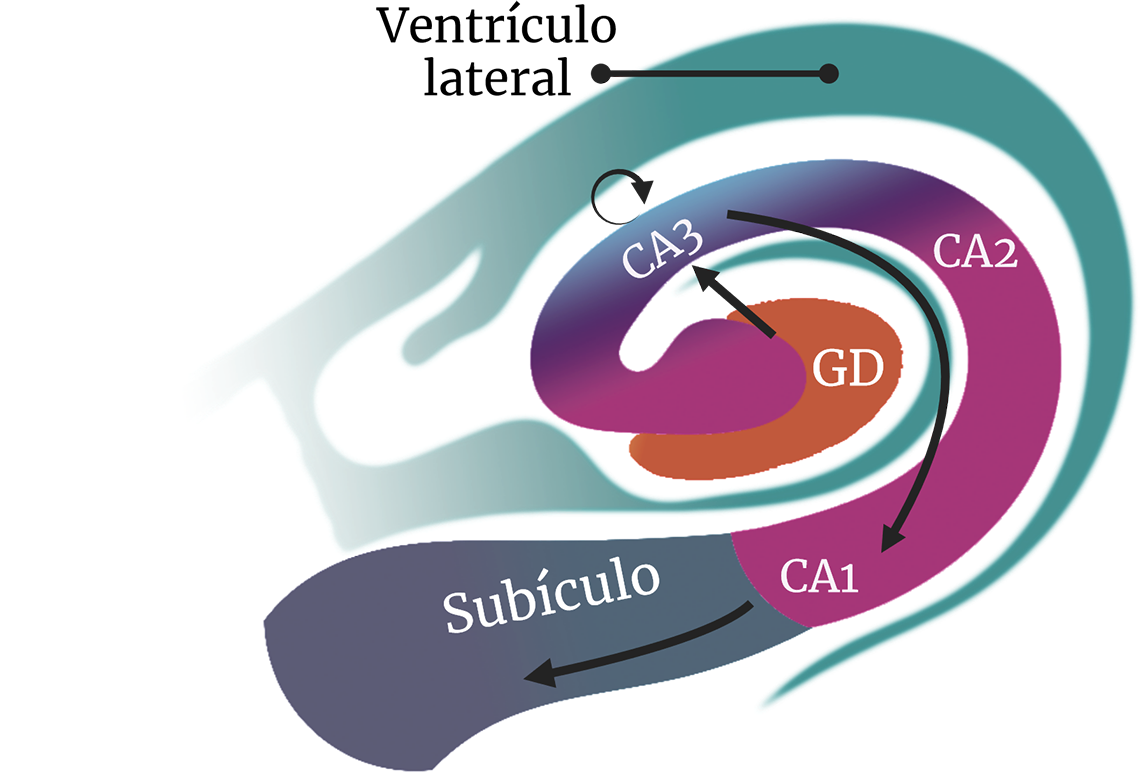
\includegraphics[keepaspectratio]{../Figures/formacion_hipocampal.png}}

}

\caption[Formación
hipocampal]{\label{fig-formacionhipocampal}Ilustración de Formación
hipocampal \colorbox{BurntOrange}{de humano}}

\end{figure}%

\end{minipage}%
%
\begin{minipage}{0.05\linewidth}
~\end{minipage}%
%
\begin{minipage}{0.55\linewidth}
Se muestran las principales estructuras en un corte coronal: \ac{gd},
\ac{ca} y el subículo. Las flechas negras representan el flujo de
información. El hipocampo se encuentra debajo del ventrículo lateral
(este último no forma parte de la formación) y su forma recuerda al
género \emph{Hippocampus} (Caballo de mar) {[}@bir2015{]}. Figura
adaptada de @andersen2007.\end{minipage}%

\end{figure}%

\todo{Vi que en las correcciones del Dr Pascal indentó los párrafos 24pt, así que agregué el indentado al escrito}
La formación hipocampal es crucial para la adquisición y consolidación
de las \href{AppendixB.qmd\#term-id-2}{memorias episódicas}
{[}@squire1992{]}, es decir, memorias de eventos, contextos, mapas
espaciales y su temporalidad {[}@tulving1972{]}. En 1885, Hermann
Ebbinghaus inició las investigaciones cuantitativas sobre la memoria y
los principios que influenciaban en su almacenamiento y olvido, como la
frecuencia y la \href{AppendixB.qmd\#term-id-58}{valencia} del estímulo
(revisado en @seel2012). @semon1921 propuso que las trazas de memoria
eran cambios físicos en las células nerviosas (un término que denominó
\href{AppendixB.qmd\#term-id-1}{engrama}), una idea fundamental para el
entendimiento de cómo las experiencias se codifican en el cerebro.
@papez1937, influenciado por el trabajo de @cannon1927 y @bard1929,
describió el ``\emph{circuito de Papez}'', un intento para identificar
un sustrato anatómico de las emociones. Casi al mismo tiempo,
@kluver1939, a partir de experimentos en primates con mescalina y la
extracción del \href{AppendixB.qmd\#term-id-59}{lóbulo temporal},
observaron efectos en el comportamiento y el procesamiento de emociones.
Klüver señaló que estas lesiones no abolían las emociones, sino que
alteraban la forma en que las emociones podían utilizarse para guiar de
manera correcta los comportamientos, una conclusión que según el mismo
Papez, confirmaban su teoría {[}@nahm1997{]}. Sin embargo, la relación
del hipocampo con la memoria se evidenció de manera más clara con el
estudio del paciente H.M. por @scoville1957. Este paciente desarrolló
amnesia anterógrada (incapacidad de formar nuevas memorias declarativas)
tras una cirugía en la que se le extirpó bilateralmente el
\href{AppendixB.qmd\#term-id-59}{lóbulo temporal medial} como
tratamiento para su epilepsia. Por otro lado, su
\href{AppendixB.qmd\#term-id-4}{memoria de corto plazo},
\href{AppendixB.qmd\#term-id-60}{memoria procedural}, así como su
habilidad de recordar \href{AppendixB.qmd\#term-id-6}{memorias
declarativas} que existían tiempo antes de su cirugía,
\colorbox{BurntOrange}{generalmente no se vieron veían afectadas}. Este
caso abrió las puertas a nuevas teorías sobre la memoria
{[}@sweatt2004{]} y resaltó la importancia del hipocampo en la
\href{AppendixB.qmd\#term-id-9}{adquisición} de
\href{AppendixB.qmd\#term-id-5}{memorias de largo plazo}, pero no
necesariamente su almacenamiento permanente (ver
Section~\ref{sec-consolidacion}). Utilizando un análisis histológico y
de imagenología más preciso del paciente H.M se observó que también
tenía severamente dañada la \href{AppendixB.qmd\#term-id-13}{amígdala} y
la \ac{ce}, además que algunas partes del hipocampo permanecían, lo que
prueba la importancia de la formación completa para llevar a cabo sus
roles cognitivos {[}@annese2014{]}.

Un aspecto fundamental de la formación hipocampal es su gran
\href{AppendixB.qmd\#term-id-15}{plasticidad sináptica} a nivel
electrofisiológico y estructural {[}@mateos-aparicio2019{]}, que le
permite reorganizarse mediante procesos como la
\todo[color=blue!40]{ya arreglé las abreviaturas en el documento. agregué un link en todas las abreviaturas para comodidad (en el pdf)}
\ac{ltp} {[}@bliss1973{]} y la \ac{ltd} {[}@ito1982{]}. Estos procesos
(Section~\ref{sec-sph}) permiten al hipocampo responder a patrones
específicos de activación con aumentos o disminuciones duraderas en la
eficacia sináptica {[}@kandel1965{]}. Además, la neurogénesis
(Section~\ref{sec-nha}), o generación de nuevas neuronas, ocurre en el
\ac{gd} incluso en la adultez de la mayoría de los mamíferos
{[}@gage2019{]}. Esta plasticidad permite al hipocampo adaptarse a
nuevas experiencias y aprendizajes {[}@epp2016{]}, así como también
ajustar la conducta en respuesta al estrés crónico
{[}@santarelli2003{]}. Los cambios sinápticos duraderos que caracterizan
estos procesos permiten que las redes neuronales del hipocampo almacenen
y utilicen información de manera eficiente y flexible {[}@kandel2014{]}.
Este ambiente altamente plástico es también esencial para la navegación
espacial y la formación de mapas cognitivos (Section~\ref{sec-mapa}),
funciones en las que el hipocampo ha demostrado ser crítico
{[}@place\_morris\_1982{]}. Además, el estrés crónico, que puede alterar
estos procesos de plasticidad, se ha relacionado con déficits cognitivos
que afectan la \href{AppendixB.qmd\#term-id-9}{adquisición},
\href{AppendixB.qmd\#term-id-10}{consolidación} y
\href{AppendixB.qmd\#term-id-12}{evocación} de las memorias
{[}@sandi2013{]}, destacando la importancia de estos procesos en la
salud mental.

\subsubsection{Anatomía y
conectividad}\label{anatomuxeda-y-conectividad}

La formación hipocampal (Figure~\ref{fig-formacionhipocampal}) tiene una
conectividad principalmente unidireccional
(Figure~\ref{fig-formacionhipocampaldos}) de naturaleza glutamatérgica
que forma un circuito cerrado
(Figure~\ref{fig-formacionhipocampaltres}), con el \ac{gd} siendo
fundamental por recibir y procesar gran parte de la información
{[}@cappaert2015{]}. Las entradas extrínsecas que modulan el circuito
hipocampal provienen de varias áreas corticales, del
\href{AppendixB.qmd\#term-id-13}{complejo amigdalino,}
\todo{No se si dejar el glosario con estos links o mejor quitarlo? originalmente lo había puesto para expandir en algunos temas que tal vez no se expanden mucho en la tesis pero que creía que podría ayudar a los lectores a tener más claridad, pero como vean...}
del \href{AppendixB.qmd\#term-id-64}{área septal medial} y del
\href{AppendixB.qmd\#term-id-26}{tálamo} {[}@chauhan2021{]}. Sus
principales \colorbox{BurntOrange}{vías aferentes} incluyen el
\href{AppendixB.qmd\#term-id-65}{giro cingulado}, el hipocampo
contralateral y la \ac{ce} {[}@schultz2014{]}.
\todo{Correcciones de estilo en este párrafo, gracias al Dr. Pascal} La
\emph{principal} vía unidireccional del hipocampo se conoce como el
\textbf{circuito trisináptico} por el número de contactos excitatorios
que lo componen (Figure~\ref{fig-formacionhipocampaldos}). El primer
relevo del circuito trisináptico ocurre en la capa molecular del
\ac{gd}, donde las dendritas de sus
\href{AppendixB.qmd\#term-id-49}{células granulares} que comprende una
vía unidireccional reciben proyecciones axónicas desde la \ac{ce}. Estos
axones entorrinales constituyen la \href{AppendixB.qmd\#term-id-61}{vía
perforante}, denominada así porque atraviesan físicamente el
\href{AppendixB.qmd\#term-id-67}{subículo}. Los axones de las células
granulares del giro dentado a su vez proyectan a \ac{ca}3 formando las
\emph{fibras musgosas}, llamadas así por sus numerosos botones
sinápticos que protruyen de sus axones, formando sinapsis de tipo
\emph{en passant} con sus neuronas blanco. Las neuronas de \ac{ca}3
finalmente transmiten su salida a través de las
\href{AppendixB.qmd\#term-id-63}{colaterales de Schaffer} a las
\href{AppendixB.qmd\#term-id-48}{neuronas piramidales} de \ac{ca}1
{[}@andersen2007{]} y también entre ellas mismas {[}@kesner2007{]}.
Además de sus complejas aferencias y conexiones intrínsecas, la
organización del hipocampo se estructura en subregiones funcionales
específicas, como describiremos más adelante.

\textbf{Entradas al hipocampo}.
\colorbox{BurntOrange}{clarificar entradas y salidas} Además de la
\textbf{vía perforante}, algunos axones procedentes de la
\colorbox{BurntOrange}{capa III} de la \ac{ce} proyectan directamente a
la región \ac{ca}1, formando la \emph{vía directa}
(Figure~\ref{fig-formacionhipocampaltres}). \ac{ca}2 recibe algunas
proyecciones de la \colorbox{BurntOrange}{capa II} de la \ac{ce}, aunque
estas son menos prominentes que las dirigidas a otras regiones del
hipocampo {[}@cappaert2015{]}. \ac{ca}3, por su parte, recibe
proyecciones de las fibras musgosas del \ac{gd} y de las neuronas
piramidales de la capa II de la \ac{ce} {[}@andersen2007{]}. \ac{ca}3,
por su parte, recibe proyecciones de las fibras musgosas, que son los
axones de las células granulares del \ac{gd} y de las neuronas
piramidales de la capa II de la \ac{ce} mediante la \emph{vía
perforante} {[}@chauhan2021{]}.

\textbf{Salidas del hipocampo}. Las células piramidales de \ac{ca}3
proyectan a \ac{ca}1 mediante las \textbf{colaterales de Schaffer}
(Figure~\ref{fig-formacionhipocampaldos}). También se observan
proyecciones desde \ac{ca}3 hacia \ac{ca}2, aunque las interacciones
entre estas regiones están menos estudiadas {[}@andersen2007{]}. Las
\textbf{colaterales de Schaffer} también realizan conexiones recurrentes
dentro de \ac{ca}3, creando un circuito complejo de interconexiones
{[}@schultz2014{]}, mientras que las proyecciones hacia otras zonas
(p.ej. subículo) se originan principalmente desde \ac{ca}1
{[}@chauhan2021{]}. \ac{ca}1 genera proyecciones
\colorbox{BurntOrange}{funcionalmente importantes} hacia la \ac{ce}
(principalmente hacia la \colorbox{BurntOrange}{capa V}) y hacia el
subículo, desempeñando un papel crucial en la transmisión de información
dentro de estos circuitos; estas conexiones forman parte del circuito
trisináptico (Figure~\ref{fig-formacionhipocampaldos}).

\begin{figure}

\begin{minipage}{0.45\linewidth}

\centering{

\pandocbounded{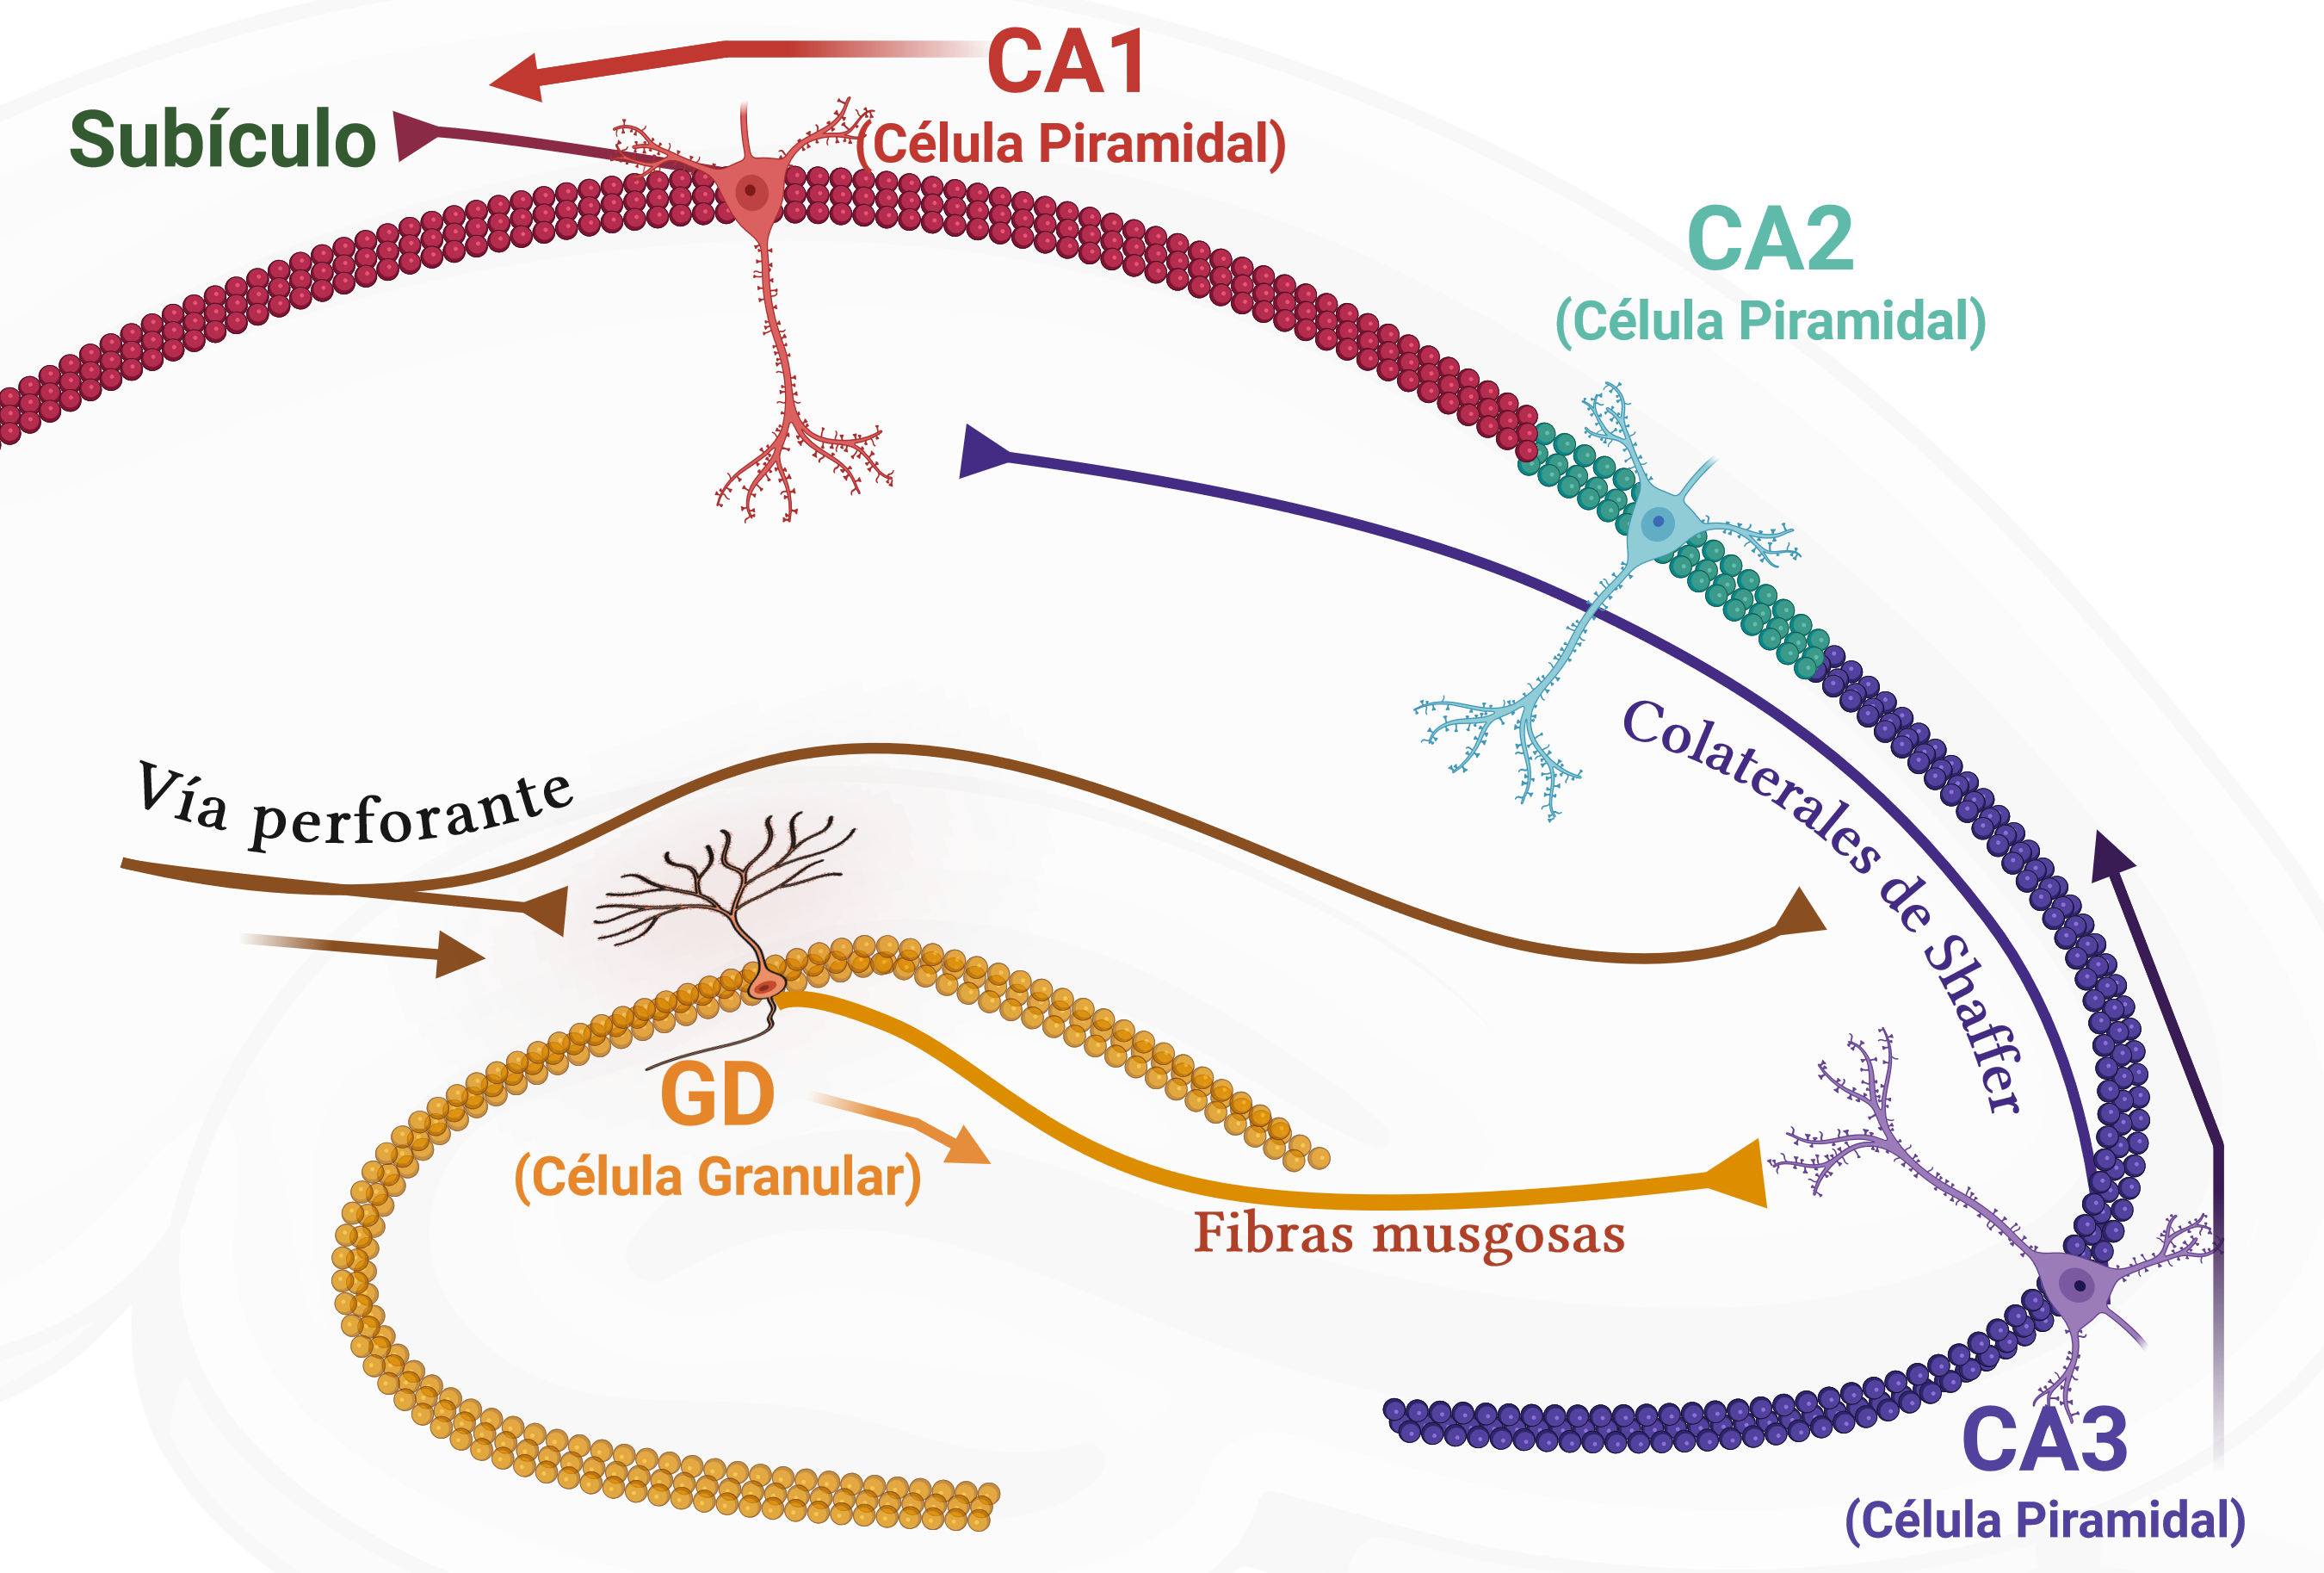
\includegraphics[keepaspectratio]{../Figures/hipocampo_neuronas.png}}

}

\subcaption{\label{fig-formacionhipocampaldos}Anatomía de la red
hipocampal. El diagrama ilustra la vía trisináptica en el hipocampo, la
cual consiste en proyecciones secuenciales desde la \ac{ce} al \ac{gd},
luego de \ac{ca}3 a \ac{ca}1 y finalmente al subículo {[}@yau2015{]}.
Figura adaptada de @andersen2007.}

\end{minipage}%
%
\begin{minipage}{0.05\linewidth}
~\end{minipage}%
%
\begin{minipage}{0.50\linewidth}

\centering{

\pandocbounded{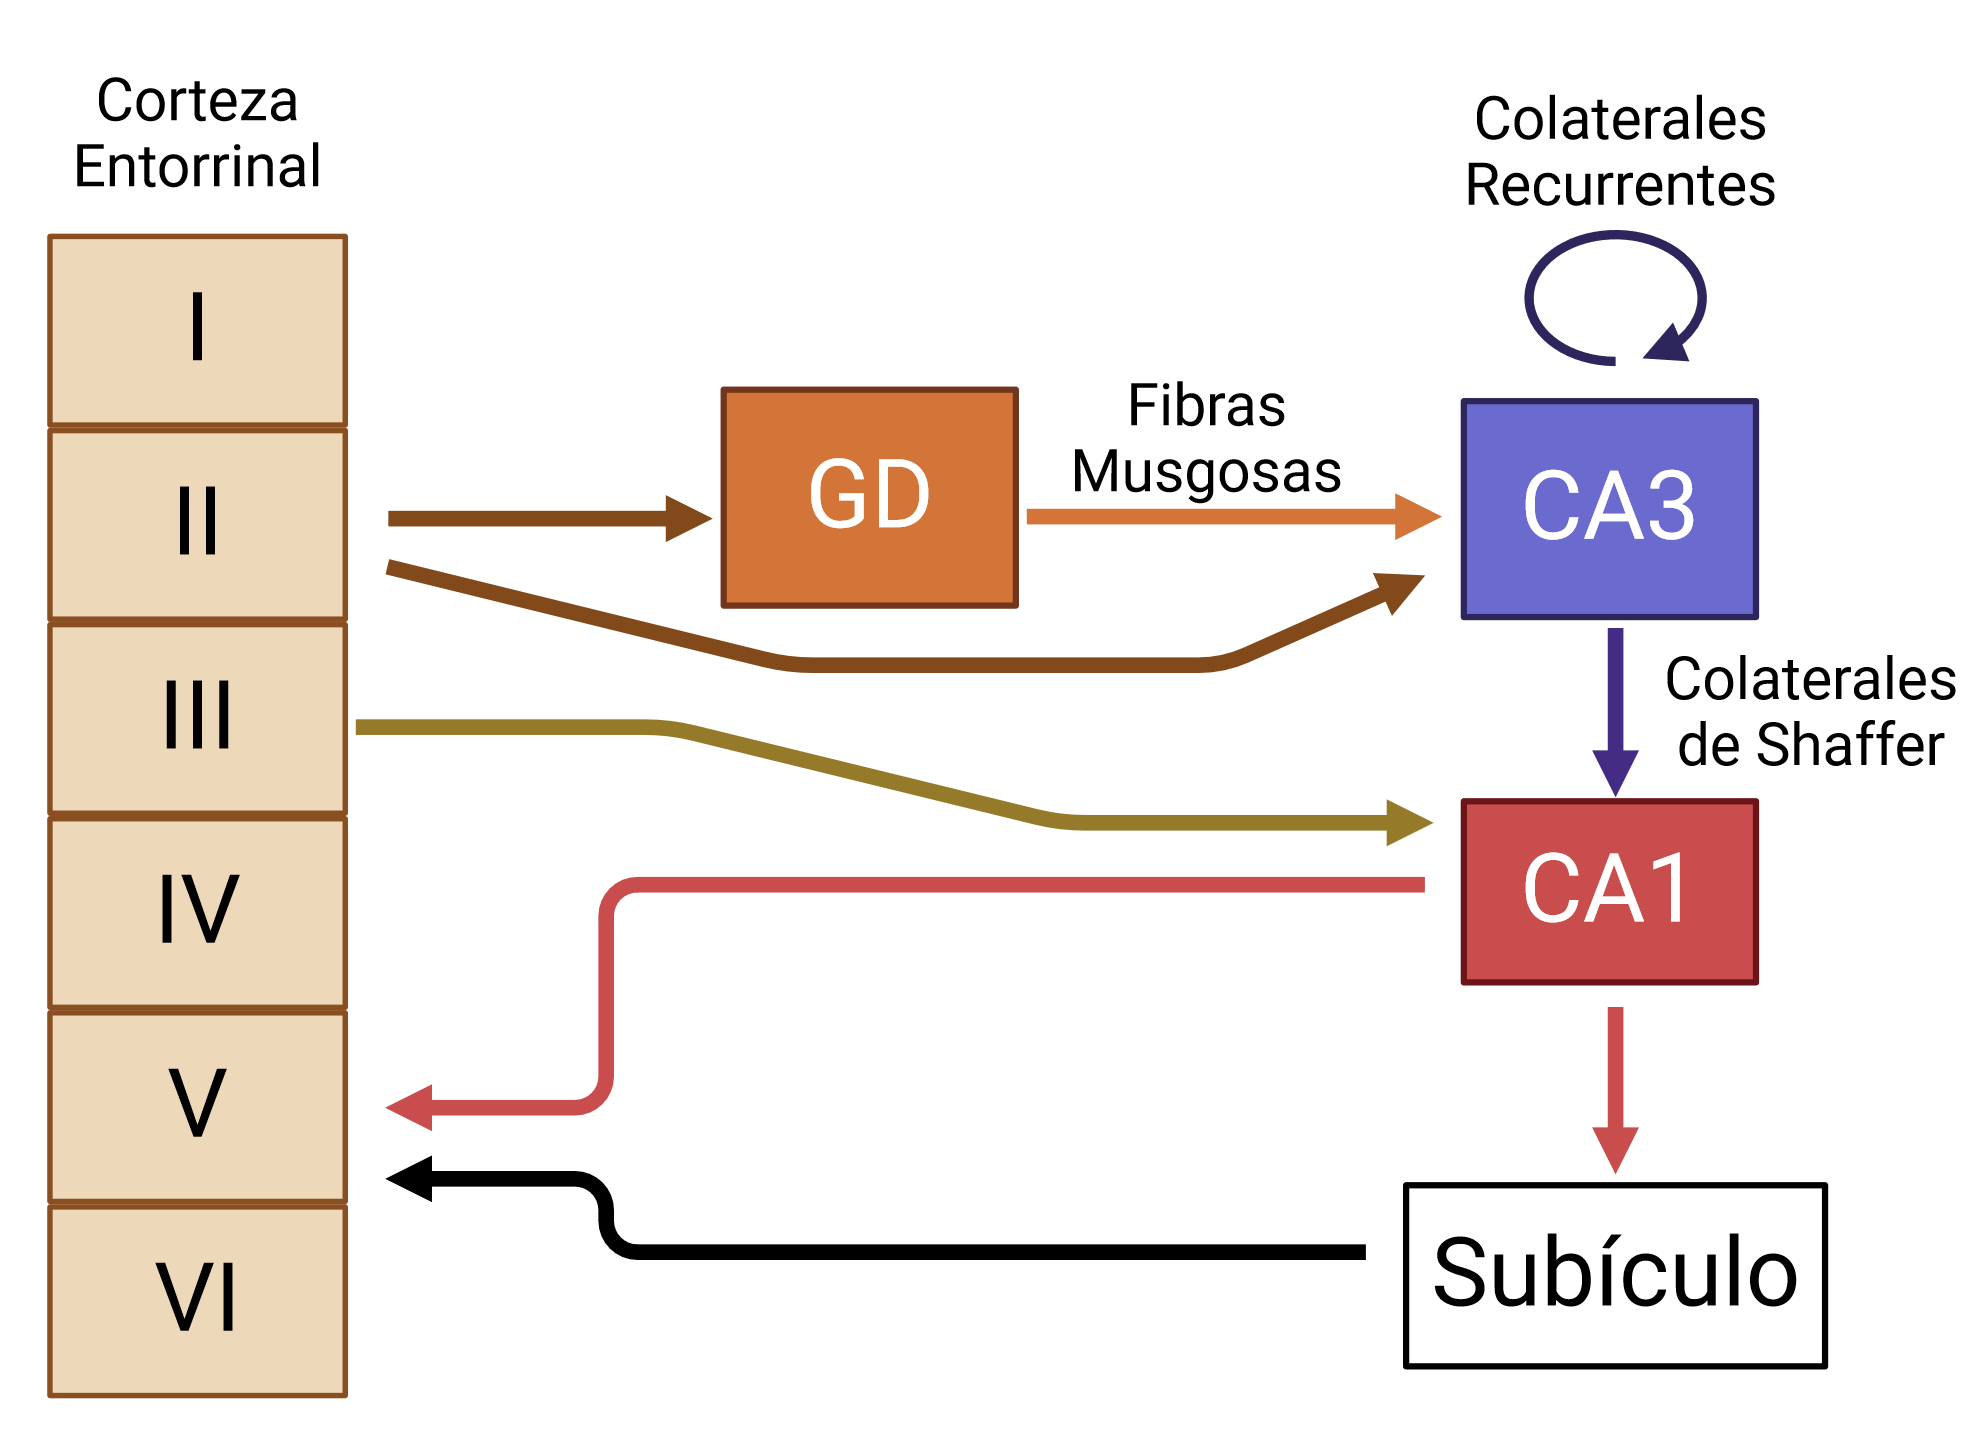
\includegraphics[keepaspectratio]{../Figures/aferencias_eferencias_hipocampo.png}}

}

\subcaption{\label{fig-formacionhipocampaltres}Esquematización de la
conectividad hipocampal. Los estímulos sensoriales externos parten de
distintas capas en la \ac{ce} y alcanzan la región \ac{ca}1 mediante dos
rutas (directa o por medio del \ac{gd}). La \ac{ce} es la principal
fuente de entrada cortical al hipocampo y el principal receptor de sus
salidas. Además, \ac{ca}3 tiene conexiones recurrentes {[}@chen2024{]}
que permiten la formación de redes autoasociativas que facilitan la
recuperación de recuerdos {[}@kesner2007{]}. Figura adaptada de
@andersen2007.}

\end{minipage}%

\caption{\label{fig-formacion}Anatomía y conectividad de la Formación
Hipocampal.}

\end{figure}%

El \ac{gd} es una región trilaminada compuesta por la capa molecular,
donde se encuentran las proyecciones dendríticas de las células
granulares, la capa granular conformada por los somas de éstas, y la
capa polimórfica {[}@andersen2007{]}. Esta última región es notable por
presentar neurogénesis continua (Figure~\ref{fig-neurogenesishipo}) a lo
largo de la vida de la mayoría de mamíferos {[}@gage2019{]}, incluyendo
al humano {[}@neurogenesis\_eriksson\_1998;
@dynamics\_spalding\_2013{]}. Las células granulares son el principal
tipo de célula en el \ac{gd}, formando capas densamente empaquetadas y
dando origen a axones que inervan \ac{ca}3; sin embargo, el \ac{gd}
también cuenta con una población importante de interneuronas gabaérgicas
(ver Figure~\ref{fig-inhibicion}). Por último, el \ac{gd} recibe
aferencias importantes de la \ac{ce} a través de la vía perforante y
proyecta a \ac{ca}3 {[}@chauhan2021{]}.

El subículo también está compuesto principalmente de neuronas
piramidales y forma una zona de transición entre \ac{ca}1
\colorbox{BurntOrange}{y la corteza} {[}@cappaert2015{]}. Esta
estructura, y en menor medida \ac{ca}1, son las principales fuentes que
proyectan fuera de la formación hipocampal hacia áreas como la \ac{ce}
(la cual se reconecta mediante el \href{AppendixB.qmd\#term-id-66}{giro
parahipocampal} con sitios
\href{AppendixB.qmd\#term-id-68}{neocorticales}), la
\href{AppendixB.qmd\#term-id-13}{amígdala}, la
\todo{estandarizar siglas de la corteza} \ac{mpfc} y la \ac{ofc}, y el
\href{AppendixB.qmd\#term-id-27}{núcleo accumbens} {[}@small2011{]}.
Además, la \ac{ce} actúa como punto de entrada para la información
sensorial y como conducto para la información procesada que se releva
nuevamente a la \href{AppendixB.qmd\#term-id-68}{neocorteza}
{[}@schultz2014{]}.

La diversidad de tipos celulares dentro de la formación hipocampal
genera diferencias moleculares que confieren distinta labilidad ante
varios tipos de agravio. Por ejemplo, en la enfermedad de Alzheimer, los
depósitos de ovillos neurofibrilares que generan neurodegeneración
afectan en un principio a \ac{ca}1 antes que otras regiones del
hipocampo {[}@small2011{]}. En los insultos agudos que involucran daño
excitotóxico, como isquemia y epilepsia, las neuronas piramidales de
\ac{ca}1 son más vulnerables, mientras que \ac{gd} y \ac{ca}3 son más
resistentes {[}@davidson2024{]}. Por otro lado, el \ac{gd} es
susceptible al estrés crónico y desórdenes de ansiedad y depresión
debido a la presencia de receptores a glucocorticoides
{[}@bartsch2012{]}. Esta vulnerabilidad diferencial subraya la
importancia de entender las funciones específicas de cada componente en
la dinámica global del hipocampo.

La función de cada estructura se puede simplificar utilizando la
analogía de @sugar2019 que destaca cómo el hipocampo procesa y edita la
información, además de jugar un papel crucial en la consolidación y
recuperación de recuerdos: las entradas desde la \emph{\ac{ce}} pueden
funcionar como una película de experiencias continuas transmitidas al
hipocampo (\emph{\ac{ca}}), que actúa como el editor de este flujo
constante de información. A través de la plasticidad neuronal modulada
por el tiempo de disparo y la reproducción, el \emph{hipocampo} extrae y
etiqueta eventos memorables para consolidarlos en la
\href{AppendixB.qmd\#term-id-2}{memoria episódica}. Durante la
recuperación, incluso con una entrada parcial o degradada de la traza de
memoria codificada, \ac{ca}3 realiza eficientemente el completamiento de
patrones e instruye a los índices de memoria en \ac{ca}1, los cuales
canalizan la reactivación cortical para el recuerdo.

\subsubsection{Aprendizaje y plasticidad}\label{sec-sph}

Los mecanismos y la hipótesis más aceptada {[}@abraham2019{]} que
explican las bases del aprendizaje en el hipocampo se engloban en el
concepto de \href{AppendixB.qmd\#term-id-15}{plasticidad neuronal}, que
se puede definir como la capacidad de las neuronas para cambiar su
actividad en respuesta a estímulos mediante la reorganización, cambio de
función o conectividad {[}@kolb2014{]}. La idea de que la fuerza de las
conexiones sinápticas subyace al fenómeno de la memoria proviene de
@cajal1894, aunque fue @hebb1949 quien postuló cómo se produce este
fortalecimiento. En su famoso postulado ``\emph{las neuronas que se
activan juntas, se conectan juntas}'', Hebb propuso que, si una neurona
A participa repetidamente en la activación de una neurona B, la conexión
sináptica entre A y B se fortalecerá. Este postulado de Hebb fue
fundamental para entender cómo una experiencia puede generar aprendizaje
a través de la plasticidad sináptica {[}@kandel2014{]}. Como
demostrarían @bliss1973 mediante el estudio de la
\href{AppendixB.qmd\#term-id-61}{vía perforante} de conejos, una
estimulación de alta frecuencia produce un incremento duradero en la
eficacia de las sinapsis, demostrando que las neuronas \emph{potencían}
sus conexiones en respuesta a un estímulo
\colorbox{BurntOrange}{fuerte, ya que éste siempre producirá respuesta en la neurona postsináptica}.
Este fenómeno es conocido como \ac{ltp}. Unos años después, @ito1982
describieron otro mecanismo por el cuál se debilitaba las conexiones
sinápticas, conocido como \ac{ltd}. Aunque la \ac{ltd} fue inicialmente
reportada en el cerebelo de conejos, este mecanismo, junto con la
\ac{ltp}, son fundamentales para el aprendizaje y la dinámica del
hipocampo, como la consolidación y mantenimiento de la memoria
{[}@dhooge2001; @fox2017{]}. Los mecanismos canónicos de \ac{ltp} y
\ac{ltd} se presentan en la Figure~\ref{fig-sph}.

\begin{figure}

\begin{minipage}{0.47\linewidth}

\centering{

\pandocbounded{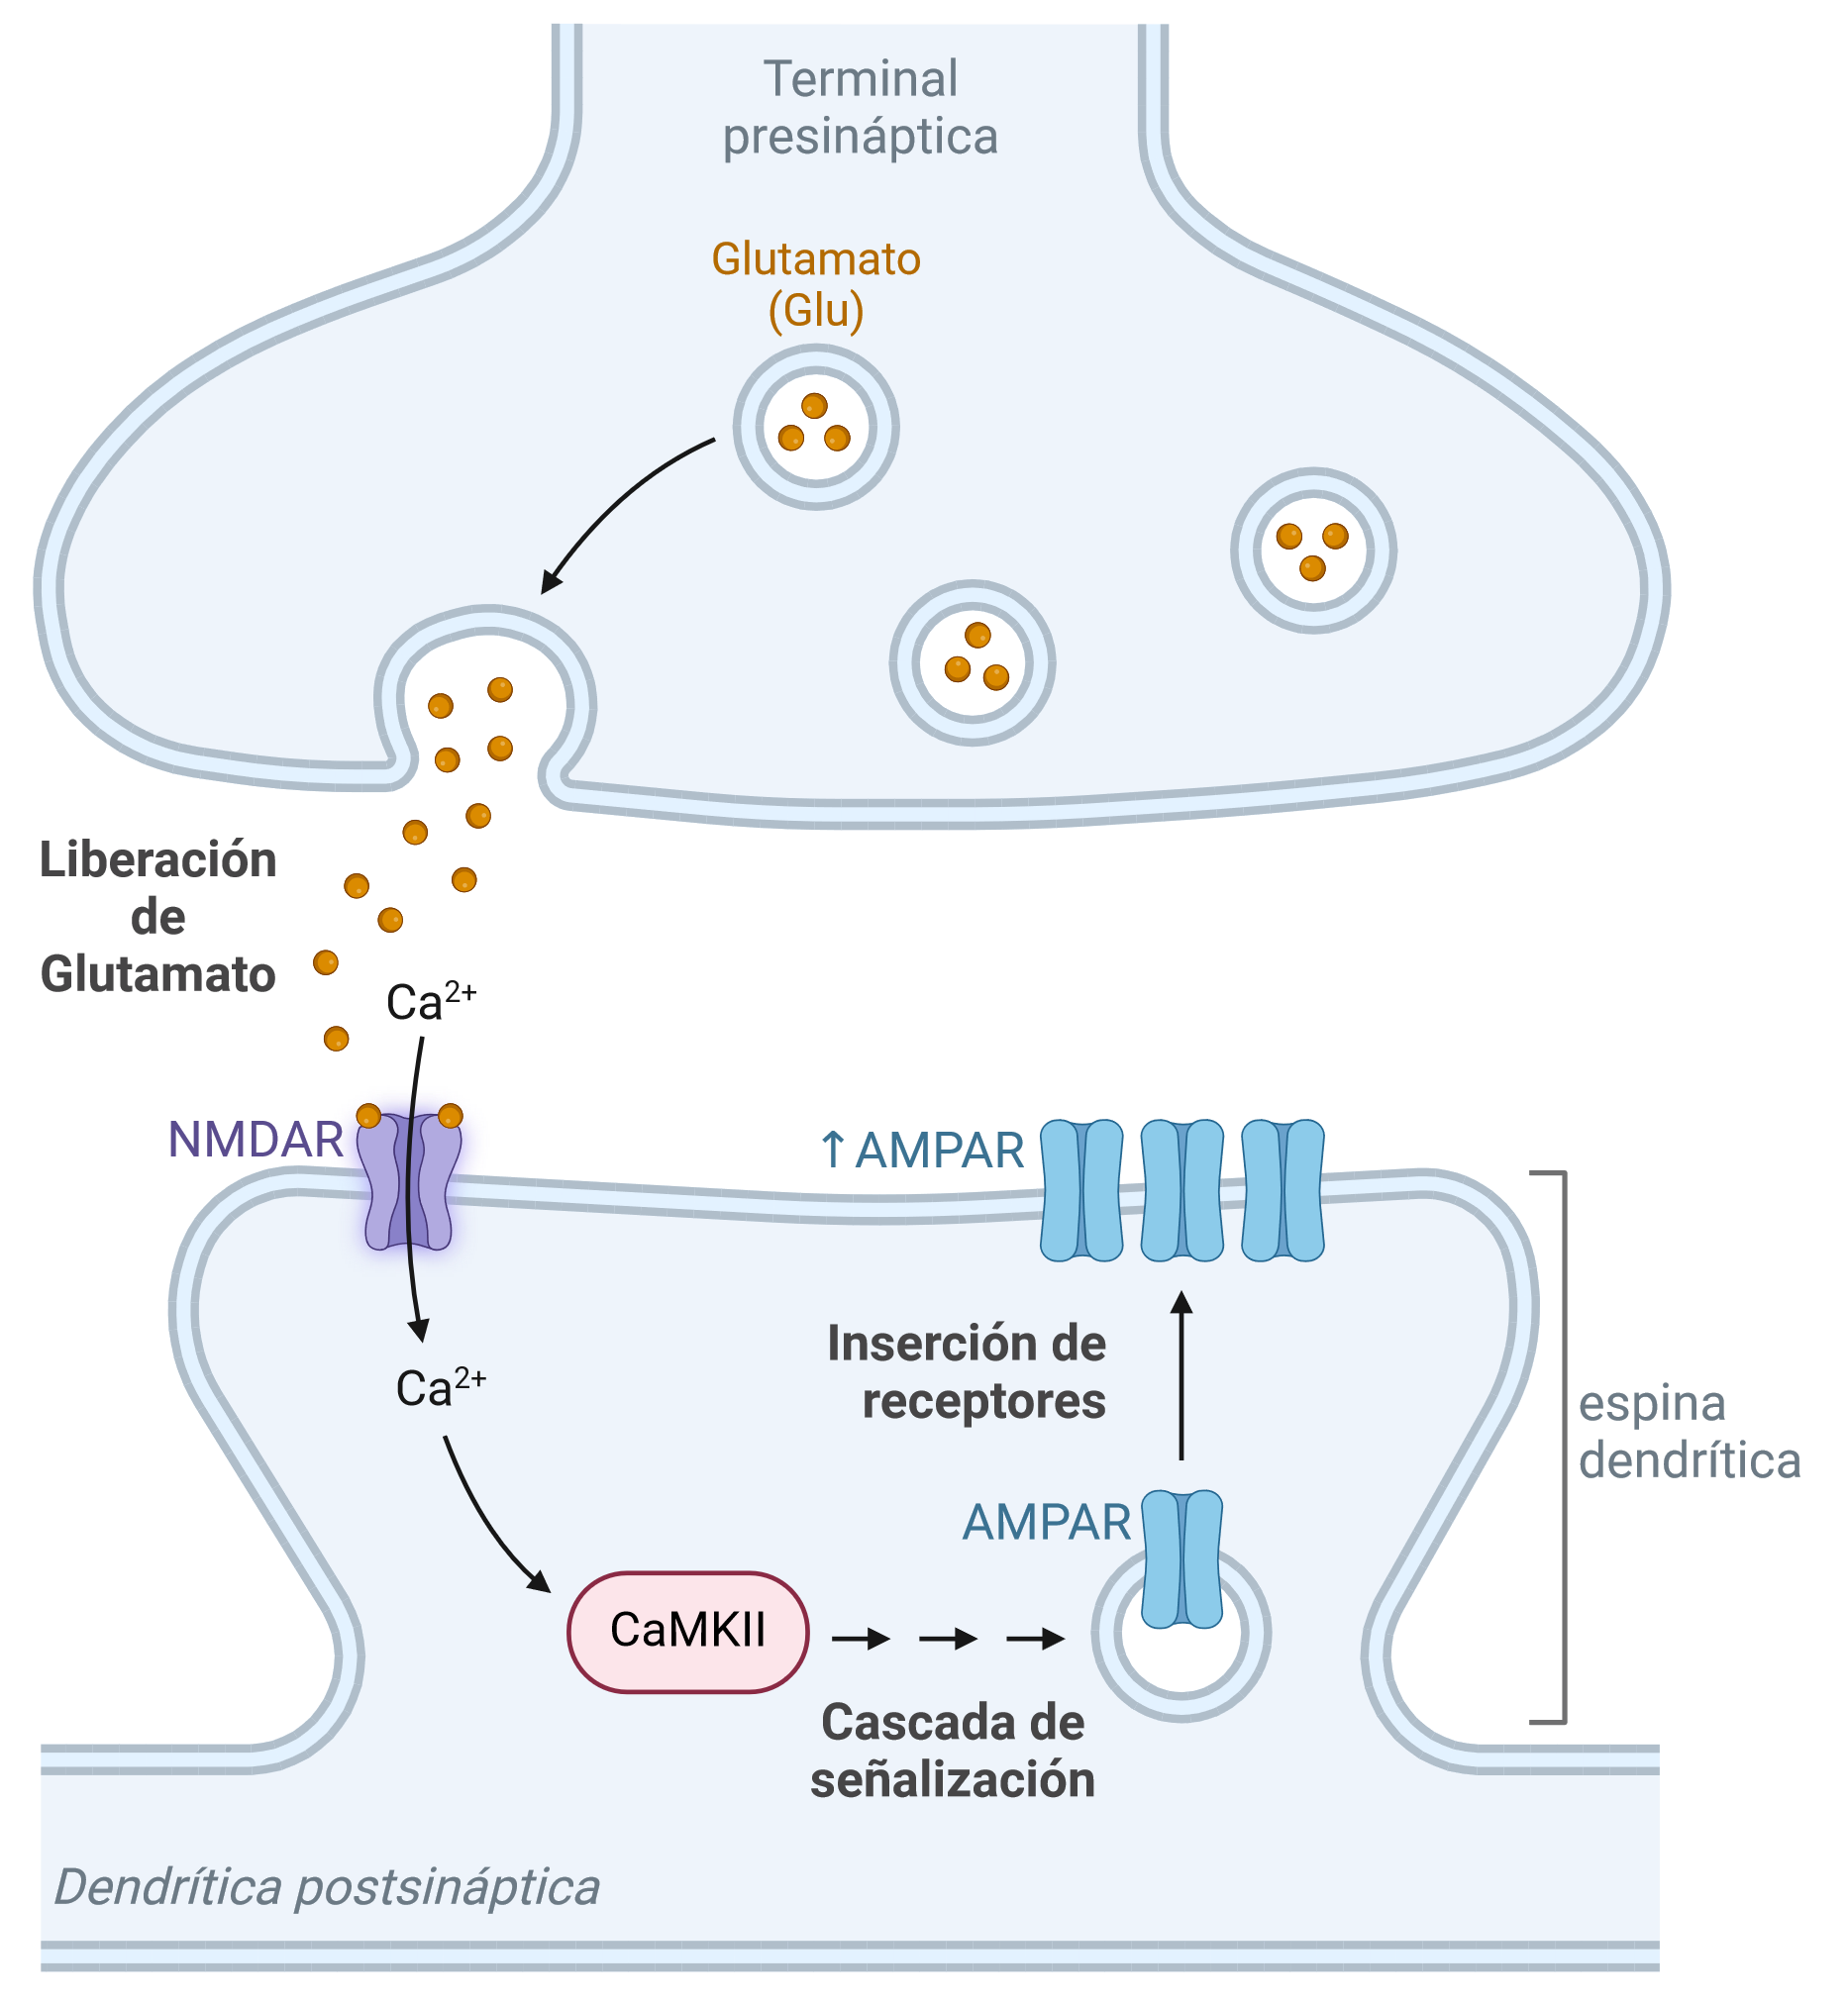
\includegraphics[keepaspectratio]{../Figures/LTP.png}}

}

\subcaption{\label{fig-LTP}LTP. Este fenómeno se induce
experimentalmente mediante la estimulación sináptica de alta frecuencia
que desencadena una serie de eventos moleculares en la neurona
postsináptica {[}@bliss1973; @lynch2004; @bliss2011; @luscher2012;
@nicoll2017{]}. Primero la estimulación de alta frecuencia induce la
liberación de glutamato desde la terminal presináptica. El glutamato se
une y activa los receptores \ac{nmda} en la membrana postsináptica. La
activación de los receptores NMDA permite la entrada de iones de calcio
(\(Ca^{2+}\)) al interior de la célula postsináptica, donde el
\(Ca^{2+}\) actúa como un segundo mensajero. Este aumento de \(Ca^{2+}\)
intracelular activa varias proteínas cinasas, como la \ac{camkii} y
\ac{pkc} que fosforilan proteínas y receptores en la membrana
postsináptica y resulta en la inserción de receptores \ac{ampa}. La
mayor densidad de receptores AMPA en la membrana fortalece la respuesta
sináptica a futuras liberaciones de glutamato (sinapsis potenciada).
Figura basada en @luscher2012}

\end{minipage}%
%
\begin{minipage}{0.05\linewidth}
~\end{minipage}%
%
\begin{minipage}{0.47\linewidth}

\centering{

\pandocbounded{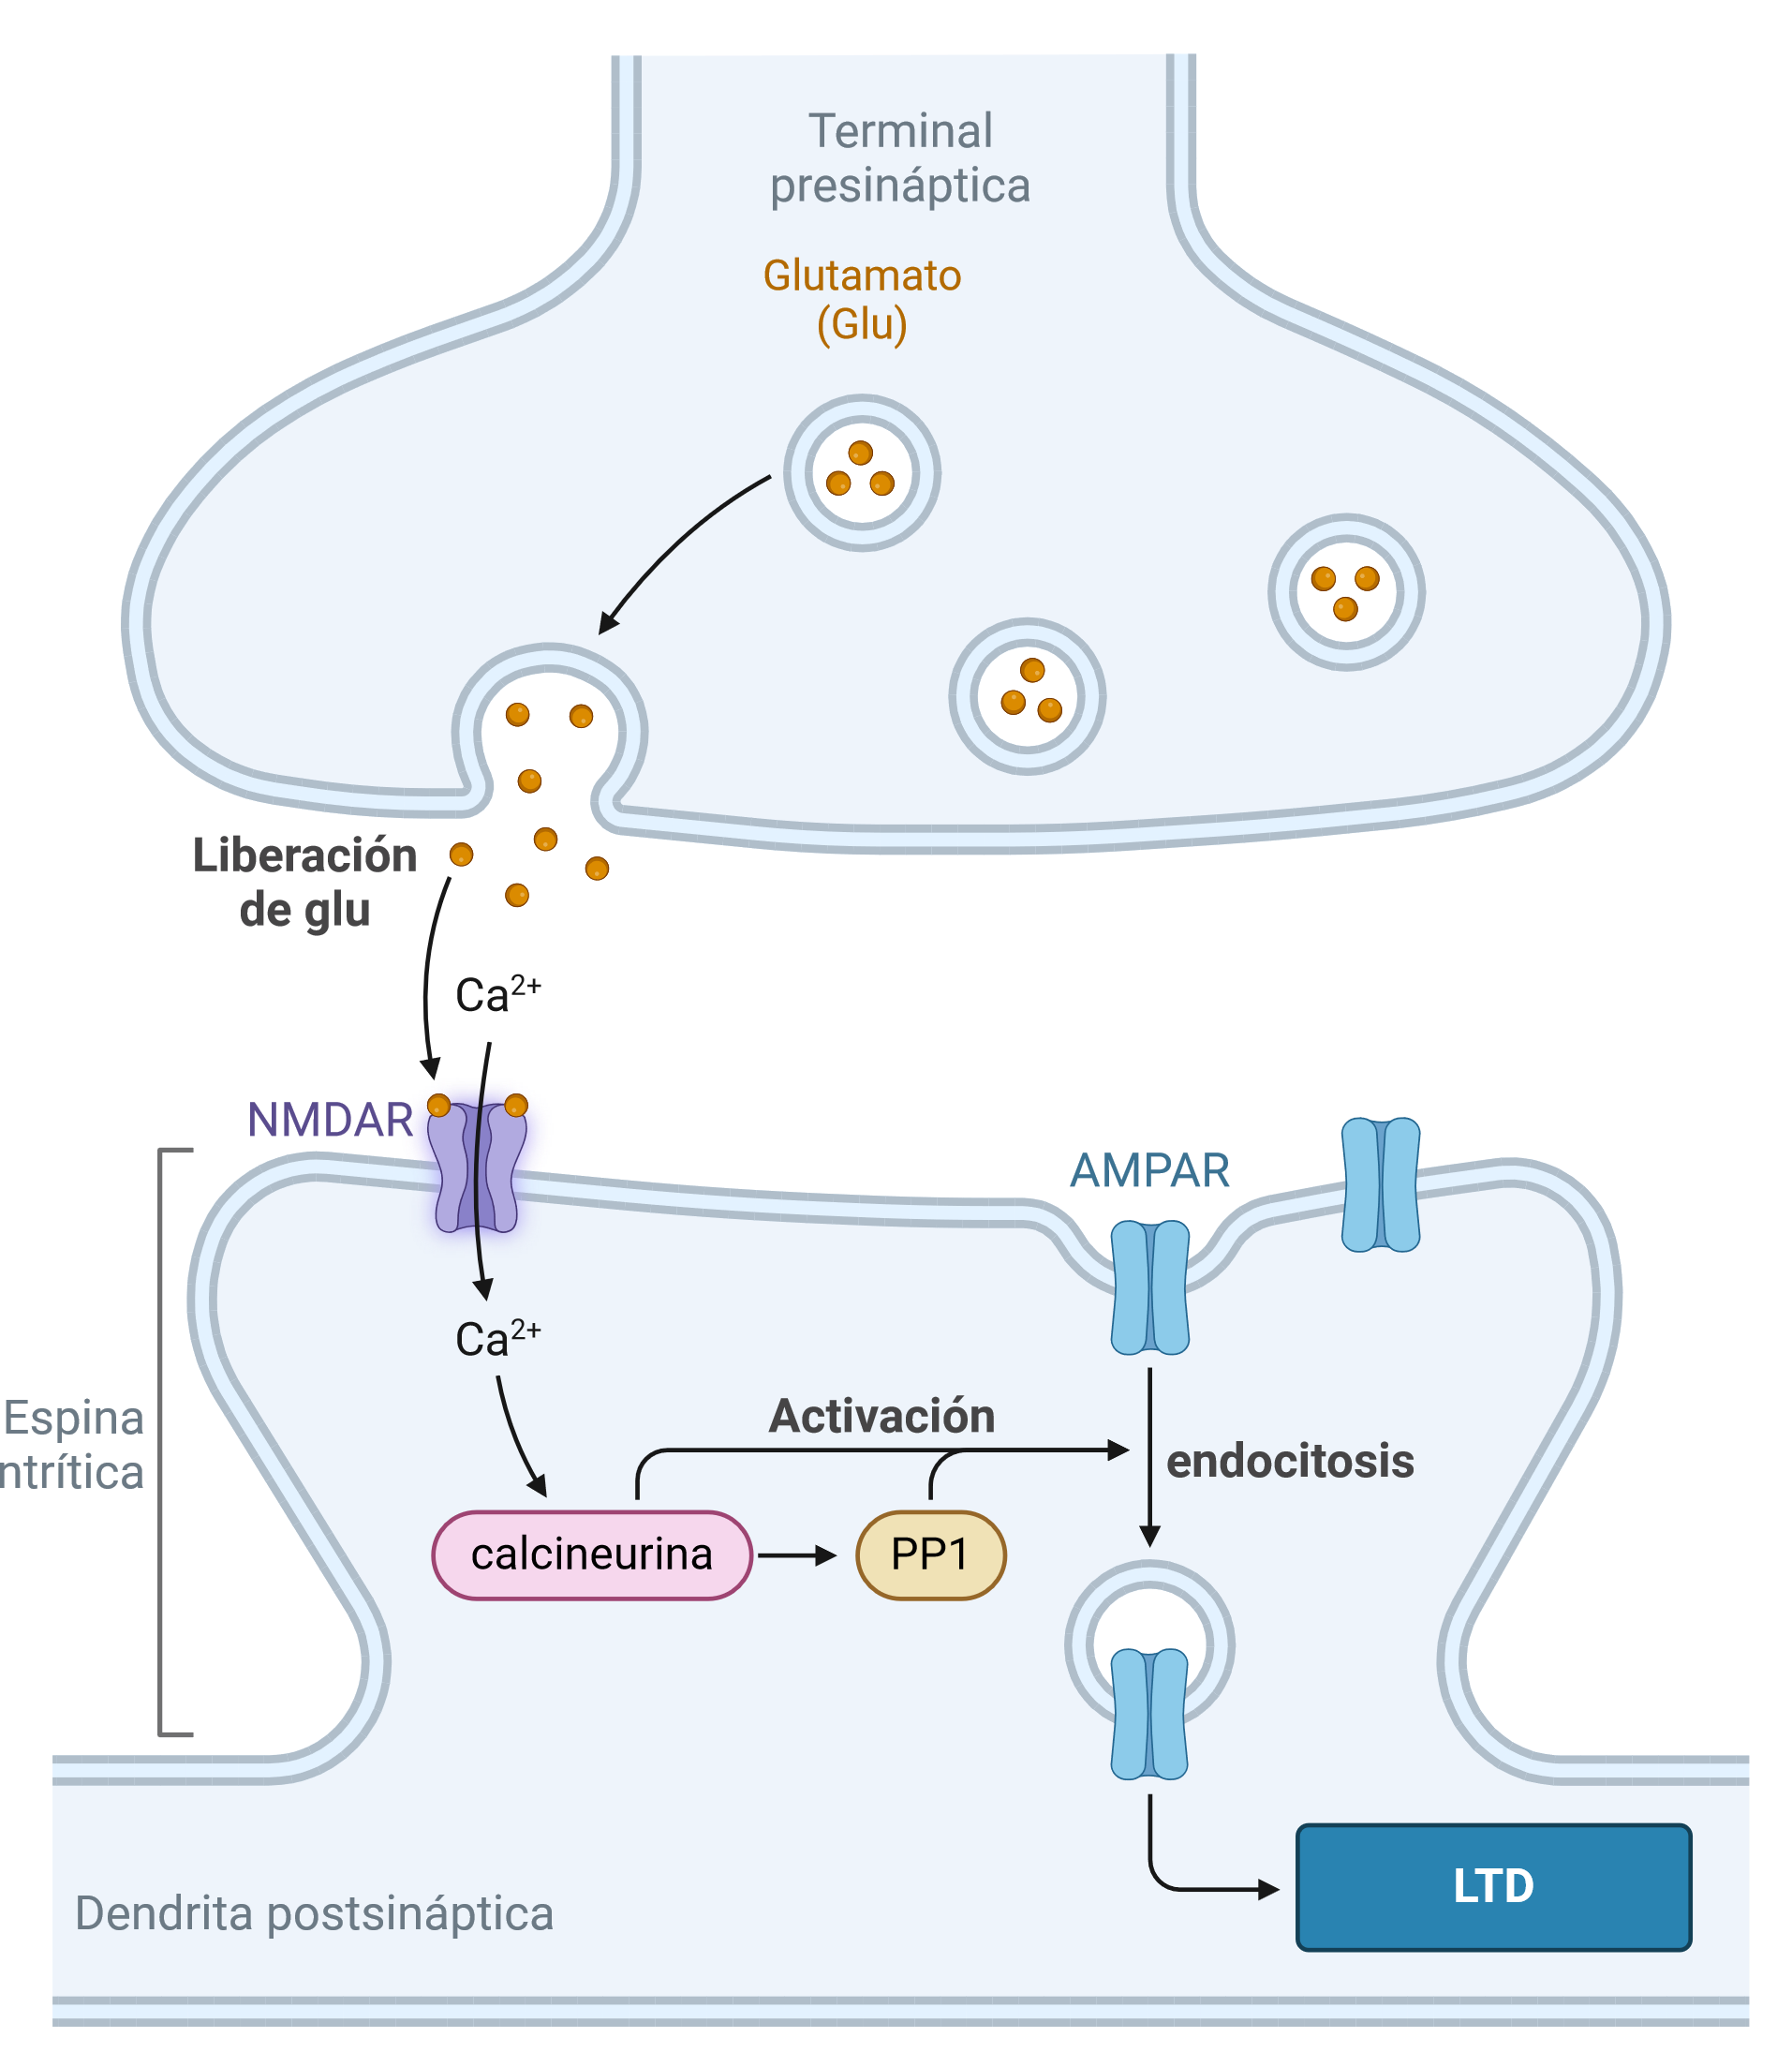
\includegraphics[keepaspectratio]{../Figures/LTD.png}}

}

\subcaption{\label{fig-LTD}LTD. Es un proceso en el cual se debilitan
las conexiones sinápticas, reduciendo su eficacia {[}@ito1982;
@bliss2011; @luscher2012{]}. La LTD se induce experimentalmente mediante
la estimulación sináptica de baja frecuencia. Al igual que en la LTP, la
estimulación sináptica provoca la liberación de glutamato y la
activación de los receptores NMDA en la neurona postsináptica. Sin
embargo, la estimulación de baja frecuencia resulta en una entrada
moderada de \(Ca^{2+}\) en la célula postsináptica, lo que conduce a la
activación de fosfatasas en lugar de cinasas. En particular, fosfatasas
como la calcineurina y \ac{pp1} son activadas por esta entrada de
\(Ca^{2+}\). Estas fosfatasas desfosforilan proteínas y receptores, lo
que provoca la internalización y degradación de los receptores AMPA en
la membrana postsináptica. La pérdida de receptores AMPA reduce la
sensibilidad de la sinapsis al glutamato, debilitando así la conexión
sináptica. Figura basada en @luscher2012}

\end{minipage}%

\caption{\label{fig-sph}Mecanismos Canónicos de LTP y LTD.}

\end{figure}%

El descubrimiento de estas manifestaciones de plasticidad neuronal
dejaba en claro que el cerebro y sus conexiones no son fijas, sino que
son ``maleables'' y se puede reorganizar a lo largo de la vida gracias a
las experiencias {[}@kandel2014{]}. Esta noción permitió avanzar en la
comprensión de cómo distintas experiencias pueden influir en múltiples
niveles ---i.e.~electrofisiológico (\ac{ltp}, \ac{ltd}), morfológico, en
proteínas, genes y en la conducta--- dentro del sistema nervioso
{[}@bailey2008{]}. Sin embargo, la primera evidencia que la plasticidad
neuronal producía cambios en la conducta fue reportada por @kandel1965
en el molusco marino \emph{Aplysia californica}. En este estudio, Kandel
y Tauc analizaron el reflejo de retirada del sifón, un comportamiento de
defensa donde el animal retrae esta estructura cuando se toca.
Encontraron que la plasticidad sináptica (cambios en la fuerza de las
conexiones) se relacionaba con dos tipos de aprendizaje y la conducta
asociada: \href{AppendixB.qmd\#term-id-55}{habituación} (reducción de la
respuesta de retirada asociada con una disminución en la eficacia
sináptica) y \href{AppendixB.qmd\#term-id-56}{sensibilización} (aumento
de la respuesta debido a un incremento en la eficacia sináptica).

Por otro lado, el primer trabajo experimental que demostró el papel de
la plasticidad en el aprendizaje mediado por el hipocampo fue realizado
por @morris1986. Utilizando el antagonista de \ac{nmda} \emph{\ac{apv}}
en el \ac{mwm}, disminuyeron \colorbox{BurntOrange}{la inducción de LTP}
\todo{en este estudio, especificar la fase de LTP} en el hipocampo de
ratas para impedir el aprendizaje espacial (dependiente del hipocampo).
Con una técnica más avanzada, @silva1992 utilizaron ratones con
mutaciones en la proteína sináptica \(\alpha\)-\ac{camkii} para reducir
la \ac{ltp} en el hipocampo y confirmaron las deficiencias en el
aprendizaje espacial. El desarrollo de la técnica de
\href{AppendixB.qmd\#term-id-69}{Cre-Lox recombinasa} {[}@sauer1988;
@orban1992{]} permitió estudios más refinados al manipular tipos
específicos de células y proteínas en momentos concretos para estudiar
la relación con la conducta {[}@tsien1996a{]}. Usando esta técnica,
@mchugh2007 crearon ratones que carecían del receptor \ac{nmda}
específicamente en las células granulares del \ac{gd}. Esta
investigación encontró que estos animales tenían deficiencias en la
prueba de discriminación contextual al miedo, otra prueba que se puede
utilizar para evaluar la función hipocampal
{[}@hernandez-mercado2022{]}.

Estas investigaciones demuestran que la plasticidad dependiente de
\ac{nmda} en el \ac{gd} es importante para el aprendizaje y la conducta.
Sin embargo, la \ac{ltp} no es un mecanismo único conservado en todos
los tipos neuronales {[}@alkadhi2021{]}, variando incluso en las
divisiones del hipocampo {[}@mcnaughton1982; @luscher2012{]}. Por
ejemplo, el fortalecimiento de las conexiones se puede inducir sin la
\colorbox{BurntOrange}{entrada} de calcio postsináptico como se ha
observado en la \ac{ltp} de las fibras musgosas {[}@mellor2001{]}.
Adicionalmente, la \ac{ltp} y \ac{ltd} no son fenómenos exclusivos de
las redes hipocampales {[}@innocenti2022{]} y su temporalidad,
regulación y función van más allá de los mecanismos canónicos
{[}@fox2017; @mateos-aparicio2019; @han2023{]} presentados en la
Figure~\ref{fig-sph}. En los últimos años se ha generado interés por el
papel de estos mecanismos plásticos en la comunicación entre el
hipocampo y otras estructuras para entender cómo se genera una memoria
episódica (Section~\ref{sec-consolidacion}). Estas investigaciones han
resaltado el papel del hipocampo para mediar la memoria en conjunto con
la \href{AppendixB.qmd\#term-id-69}{neocorteza} {[}@kitamura2017;
@tonegawa2018; @goto2021{]}. Sin embargo,
\hyperref[callout-reconsolidacion]{hay otros mecanismos que regulan la
memoria y el comportamiento} más allá de la LTP/LTD.

\subsubsection{Consolidación de sistemas}\label{sec-consolidacion}

Décadas de investigación han demostrado que la formación hipocampal está
implicada en diversas funciones cognitivas, incluyendo el aprendizaje
contextual {[}@amelchenko2023{]}, la navegación espacial
{[}@place\_morris\_1982{]}, el discernimiento de contextos similares o
\emph{separación de patrones} {[}@nakashiba2012{]} y los procesos de
memoria que surgen como resultado de la integración, separación y
completamiento de la información proyectada y transmitida a través de
sus distintas subregiones {[}@mcavoy2015{]}. Estas funciones del
hipocampo están estrechamente vinculadas con su papel en la memoria
episódica, como se ha sugerido en investigaciones históricas y
contemporáneas.

Como se mencionó anteriormente, la investigación de @scoville1957
indicaba que el lóbulo temporal medial, que alberga la formación
hipocampal, es crucial para la
\href{AppendixB.qmd\#term-id-10}{consolidación} (estabilización de la
información adquirida) y la
\href{AppendixB.qmd\#term-id-12}{recuperación} de memorias
\href{AppendixB.qmd\#term-id-6}{declarativas} {[}@berdugo-vega2023{]}.
Aunque @scoville1957 originalmente concluyeron que el estudio demostraba
la importancia del hipocampo anterior y el giro hipocampal en la
formación y retención de nuevas experiencias, más tarde se demostró que
la operación de H.M. no se limitó solo al hipocampo. @corkin1997
revelaron que la cirugía se extendía al complejo
\href{AppendixB.qmd\#term-id-13}{amigdalino}, la \ac{ce}, partes de la
corteza \href{AppendixB.qmd\#term-id-66}{perirrinal} y porciones
rostrales del hipocampo, así como partes de la corteza
\href{AppendixB.qmd\#term-id-66}{parahipocampal}. Sin embargo,
@zola-morgan1986 presentaron el caso del paciente R.B., quien desarrolló
amnesia anterógrada severa después de un episodio isquémico que resultó
en una lesión bilateral limitada a la región \ac{ca}1 del hipocampo.
Estos hallazgos subrayan la importancia del hipocampo en la memoria, lo
que lleva a una comprensión más profunda del proceso de
\href{AppendixB.qmd\#term-id-10}{consolidación} de memorias a nivel de
sistemas. La consolidación de sistemas es un proceso por el cual las
memorias inicialmente dependientes del hipocampo se estabilizan en otras
áreas de la \href{AppendixB.qmd\#term-id-68}{corteza cerebral}
{[}@squire1992{]}. Diversos modelos presentados a continuación han
explicado la dinámica de este proceso, destacando la importancia de la
formación hipocampal y su interacción con la neocorteza en la memoria.
Aunque estos modelos se enfocan en diferentes aspectos de la función del
hipocampo, todos reconocen su papel esencial en la consolidación de
memorias episódicas.

\begin{tcolorbox}[enhanced jigsaw, colframe=quarto-callout-warning-color-frame, left=2mm, bottomrule=.15mm, rightrule=.15mm, arc=.35mm, toprule=.15mm, leftrule=.75mm, breakable, opacityback=0, colback=white]

\vspace{-3mm}\textbf{\textbf{Modelo estándar de consolidación}}\vspace{3mm}

El primero en proponer formalmente este modelo fue David @marr1971,
quien utilizando modelamiento computacional planteó que el hipocampo
podía almacenar temporalmente la información antes de su procesamiento
adicional en la \href{AppendixB.qmd\#term-id-68}{neocorteza} para el
almacenamiento a largo plazo. Evidencia experimental {[}@alvarez1994;
@knowlton1998{]} parecía apoyar esta teoría, indicando que el hipocampo
actúa como un almacén temporal para las memorias recientes y que, con el
tiempo, estas memorias se transfieren a la neocorteza para su
almacenamiento a largo plazo. Una vez que las memorias han sido
consolidadas en la neocorteza, el hipocampo ya no es necesario para su
recuperación. Sin embargo, esta ``transferencia'' de memoria del
hipocampo a la neocorteza es un concepto que otros modelos de
consolidación cuestionan {[}@willshaw2015; @winocur2010; @kandel2014{]}.

\end{tcolorbox}

\begin{tcolorbox}[enhanced jigsaw, colframe=quarto-callout-note-color-frame, left=2mm, bottomrule=.15mm, rightrule=.15mm, arc=.35mm, toprule=.15mm, leftrule=.75mm, breakable, opacityback=0, colback=white]

\vspace{-3mm}\textbf{\textbf{Modelo de la traza múltiple}}\vspace{3mm}

Este modelo {[}@nadel1997; @nadel2000; @nadel2007{]} propone que el
papel del hipocampo no se limita únicamente a la
\href{AppendixB.qmd\#term-id-10}{consolidación} inicial de la memoria,
extendiendo su función en la \href{AppendixB.qmd\#term-id-12}{evocación}
de la memoria. Esta evocación puede resultar en la formación de nuevas
trazas en el hipocampo, un concepto conocido como
\href{AppendixB.qmd\#term-id-11}{reconsolidación}. El impacto de este
fenómeno sobre la conducta \hyperref[callout-reconsolidacion]{se expande
más adelante}.

La principal diferencia con el \hyperref[callout-modeloestandar]{modelo
estándar de consolidación} es que esta teoría sostiene que el hipocampo
proporciona el contexto espacial y temporal del recuerdo mientras la
memoria siga siendo accesible {[}@kandel2014{]}, no solo en las primeras
etapas de la consolidación como propone el modelo estándar. Además, el
modelo sugiere que las memorias antiguas, que han sido
\href{AppendixB.qmd\#term-id-12}{evocadas} y reforzadas repetidamente,
pueden desarrollar múltiples trazas en el hipocampo. Estas trazas
adicionales hacen que las memorias sean más resistentes al olvido
{[}@lee2009{]}. Sin embargo, con el tiempo estas memorias tienden a
perder detalles específicos y a convertirse en representaciones más
abstractas o generalizadas. Investigaciones más recientes
{[}@lesburgueres2011; @kitamura2017; @goto2021{]} parecen soportar esta
hipótesis, indicando que el hipocampo es necesario en las primeras fases
del aprendizaje, en la maduración de la memoria hacia la neocorteza y en
la \href{(\#callout-reconsolidacion)}{evocación y reconsolidación} de la
memoria.

\end{tcolorbox}

\begin{tcolorbox}[enhanced jigsaw, colframe=quarto-callout-tip-color-frame, left=2mm, bottomrule=.15mm, rightrule=.15mm, arc=.35mm, toprule=.15mm, leftrule=.75mm, breakable, opacityback=0, colback=white]

\vspace{-3mm}\textbf{\textbf{Teoría de Construcción de escenario}}\vspace{3mm}

En esta teoría {[}@hassabis2007; @hassabis2009{]} se expande la función
y relevancia del hipocampo y la neocorteza más allá de la consolidación
de la memoria y destaca su papel crucial en la imaginación y la
simulación de eventos futuros {[}@quiroga2020{]}. De acuerdo con esta
teoría, el hipocampo permite a los individuos crear y manipular
escenarios mentales, esencial tanto para recordar el pasado como para
planificar el futuro. Esta capacidad para construir escenarios puede
ayudar en la toma de decisiones y en la resolución de problemas al
permitir a las personas imaginar diferentes posibilidades y sus
consecuencias. Además, esta teoría implica que la evocación de recuerdos
pasados a partir de la información almacenada es un proceso
``reconstructivo'' {[}@maguire2013{]} en lugar de una recuperación de
una memoria perfecta. Esta idea resalta que las memorias pueden ser
\emph{reformadas} continuamente por nuevas experiencias
{[}@moscovitch2022{]} y alterar las conductas {[}@gilboa2021{]} y
estados emocionales asociadas a los recuerdos {[}@cowan2021{]}.

\end{tcolorbox}

\subsubsection{Mapas Cognitivos}\label{sec-mapa}

Otra teoría importante sobre la función de la formación hipocampal es
que genera una representación neuronal del entorno espacial, creando un
\emph{mapa cognitivo} {[}@hippocampus\_okeefe\_1978{]}. Esta idea fue
propuesta por @tolman1948 y desarrollada gracias al descubrimiento de
las ``células de lugar'' {[}@okeefe1971{]} en el hipocampo
(principalmente en las regiones \ac{ca}1 y \ac{ca}3) {[}@fox1975{]}.
Estas neuronas se activan de manera específica cuando un animal se
encuentra en una ubicación particular y permite generar este mapa como
una representación mental del entorno físico de un individuo.

Tal \emph{mapa cognitivo} permite a los organismos navegar y comprender
su entorno al codificar información sobre relaciones espaciales y puntos
de referencia {[}@andersen2007{]}, lo cual explica por qué ratones con
lesiones en el hipocampo no pueden generar estrategias espaciales para
recordar la posición de escape en un laberinto
{[}@developments\_morris\_1984{]}. La teoría del mapa cognitivo tiene
profundas implicaciones para comprender no solo la memoria espacial,
sino también cómo el cerebro organiza y recupera información relacional
{[}@eichenbaum2004{]}: La formación hipocampal ayuda a asociar elementos
de una experiencia (qué pasó, dónde y cuándo) con un contexto y tiempo
específico {[}@whittington2020{]}. En consecuencia, al recordar una
memoria, la formación hipocampal ayuda a reconstruir la experiencia
reuniendo los diferentes elementos de la memoria y permite a los
individuos usar la información de maneras nuevas y flexibles
{[}@eichenbaum2017{]}. Este procesamiento relacional ocurre durante la
codificación, pero se hace evidente durante la recuperación de la
memoria en diferentes circunstancias {[}@lee2009{]}, una idea asociada
con la \emph{flexibilidad} en la memoria, ya que podemos recordar hechos
y eventos desde contextos diferentes al aprendizaje inicial
{[}@cognitive\_uddin\_2021{]}. La relevancia de esta flexibilidad de la
memoria sobre la salud mental \hyperref[callout-reconsolidacion]{se
explica a continuación}.

\begin{tcolorbox}[enhanced jigsaw, colframe=quarto-callout-note-color-frame, left=2mm, bottomrule=.15mm, rightrule=.15mm, arc=.35mm, toprule=.15mm, leftrule=.75mm, breakable, opacityback=0, colback=white]

\vspace{-3mm}\textbf{\textbf{Evocación, reconsolidación y distrés}}\vspace{3mm}

\hyperref[callout-trazamultiple]{Como se mencionó previamente}, la
recuperación de una memoria
(\href{AppendixB.qmd\#term-id-12}{\emph{evocación}}) y la
\href{AppendixB.qmd\#term-id-11}{\textbf{reconsolidación}} de una
memoria son procesos distintos, pero relacionados con la gestión de los
recuerdos y la conducta.

La \textbf{\emph{evocación}} se puede definir como \emph{la recuperación
de una memoria por la cual se accede y se trae a la conciencia un
recuerdo consolidado}. Este proceso implica la activación de las redes
neuronales (\href{AppendixB.qmd\#term-id-1}{engramas}) que codificaron
originalmente la información {[}@tonegawa2018{]}, particularmente en el
hipocampo y la neocorteza. La memoria evocada permanece estable durante
su recuperación.

La \textbf{\emph{reconsolidación}} se refiere a un fenómeno que puede
ocurrir después de que una memoria ha sido evocada. En este caso, la
memoria es temporalmente inestable y susceptible a modificaciones,
permitiendo actualizar el recuerdo original {[}@tronson2007;
@lee2009{]}. En este caso, la memoria tiene que ser estabilizada
nuevamente mediante la síntesis de proteínas \emph{de novo}
{[}@sara2000; @nader2000; @lods2021{]} por mecanismos similares a la
\href{AppendixB.qmd\#term-id-11}{consolidación} inicial de la memoria
(activación de receptores \ac{nmda} y modulación de la plasticidad
sináptica).

La actualización de la memoria durante la reconsolidación es un punto de
interés para el tratamiento de padecimientos mentales donde el fallo en
la flexibilidad de la memoria genera
\href{AppendixB.qmd\#term-id-18}{distrés}. El \emph{distrés} se refiere
a una respuesta biológica o emocional aversiva para el individuo y se
diferencia del estrés en que este último puede ser adaptativo para la
función cognitiva {[}@vangerven2016{]} o la neocorteza
{[}@kriesche2023{]}. La experiencia subjetiva desagradable del distrés
incluye estados emocionales que pueden inducir padecimientos como
ansiedad y depresión {[}@ridner2004{]}, ambos asociados a una
incapacidad \emph{percibida} de afrontar las demandas ambientales que
generan cambios en el estado emocional, malestar físico y diversas
alteraciones cognitivas {[}@matthews2016{]}.

\end{tcolorbox}

\subsubsection{Neurogénesis adulta en el Giro dentado}\label{sec-nha}

El \ac{gd} es una de las pocas áreas del cerebro adulto que genera
constantemente nuevas neuronas, un fenómeno conocido como \ac{nha}. Este
descubrimiento desafió la antigua creencia de que el cerebro adulto es
incapaz de generar nuevas neuronas a lo largo de la vida, creencia que
se originó con la propuesta de la ``\emph{doctrina de la neurona}''
basada en el trabajo de Santiago Ramón y Cajal. En efecto, en el año
1913, Ramón y Cajal escribió: ``\emph{En el adulto, las terminales
nerviosas son fijas e inmutables. Todo puede morir, pero nada se puede
regenerar}'' {[}historia del concepto revisada en @kumar2019{]}.
Utilizando timidina tritiada, el estudio pionero de @altman1965 presentó
la primera evidencia de la presencia de células no diferenciadas en la
capa granular del \ac{gd} en el hipocampo de ratas adultas. Décadas
después, utilizando técnicas de inmunohistoquímica en cerebros
\emph{post -mortem} de pacientes con cáncer que habían recibido
\ac{brdu} (análogo de la timidina) para fines diagnósticos,
@neurogenesis\_eriksson\_1998 mostraron por primera vez evidencia de
neurogénesis en el \ac{gd} de humanos. Estudios subsecuentes demostraron
que este fenómeno no solo es crucial para la plasticidad hipocampal
{[}@toda2018{]} y probablemente para la adquisición de memorias
dependientes del hipocampo {[}@suarez-pereira2015{]}, sino que también
se ha vinculado con la regulación del estado de ánimo y la respuesta al
estrés {[}@anacker2017{]}.

La NHA implica la proliferación de células progenitoras neurales, su
diferenciación en neuronas y su integración eventual en circuitos
neuronales funcionales, como se describe más a detalle en la
Figure~\ref{fig-neurogenesishipo}. La NHA también es regulada por otros
tipos de células no ilustradas en la Figure~\ref{fig-neurogenesishipo},
incluyendo interneuronas {[}@groisman2020{]}, células gliales y la
matriz extracelular {[}@cope2019{]}. Las interneuronas del \ac{gd}
modulan la excitabilidad neuronal, influyendo en un balance adecuado de
excitación e inhibición crucial para la supervivencia y la maduración de
las nuevas neuronas {[}@barrutieta-arberas2023{]}. Además, juegan un
papel en la sincronización de la actividad neuronal en redes
hipocampales (Figure~\ref{fig-inhibicion}). Por otro lado, los
astrocitos son cruciales para la supervivencia y el crecimiento de las
células en desarrollo por varios mecanismos {[}@elsayed2015{]}, como el
mantenimiento de la homeostásis del medio extracelular y la secreción de
factores neurotróficos ---p.~ej. el \ac{bdnf}--- que promueven la
supervivencia, proliferación, y diferenciación {[}@araki2021{]}
neuronal. La matriz extracelular, por otro lado, proporciona un entorno
tridimensional que guía la migración y la integración de las nuevas
neuronas en el circuito {[}@cope2019{]}.

\begin{figure}

\centering{

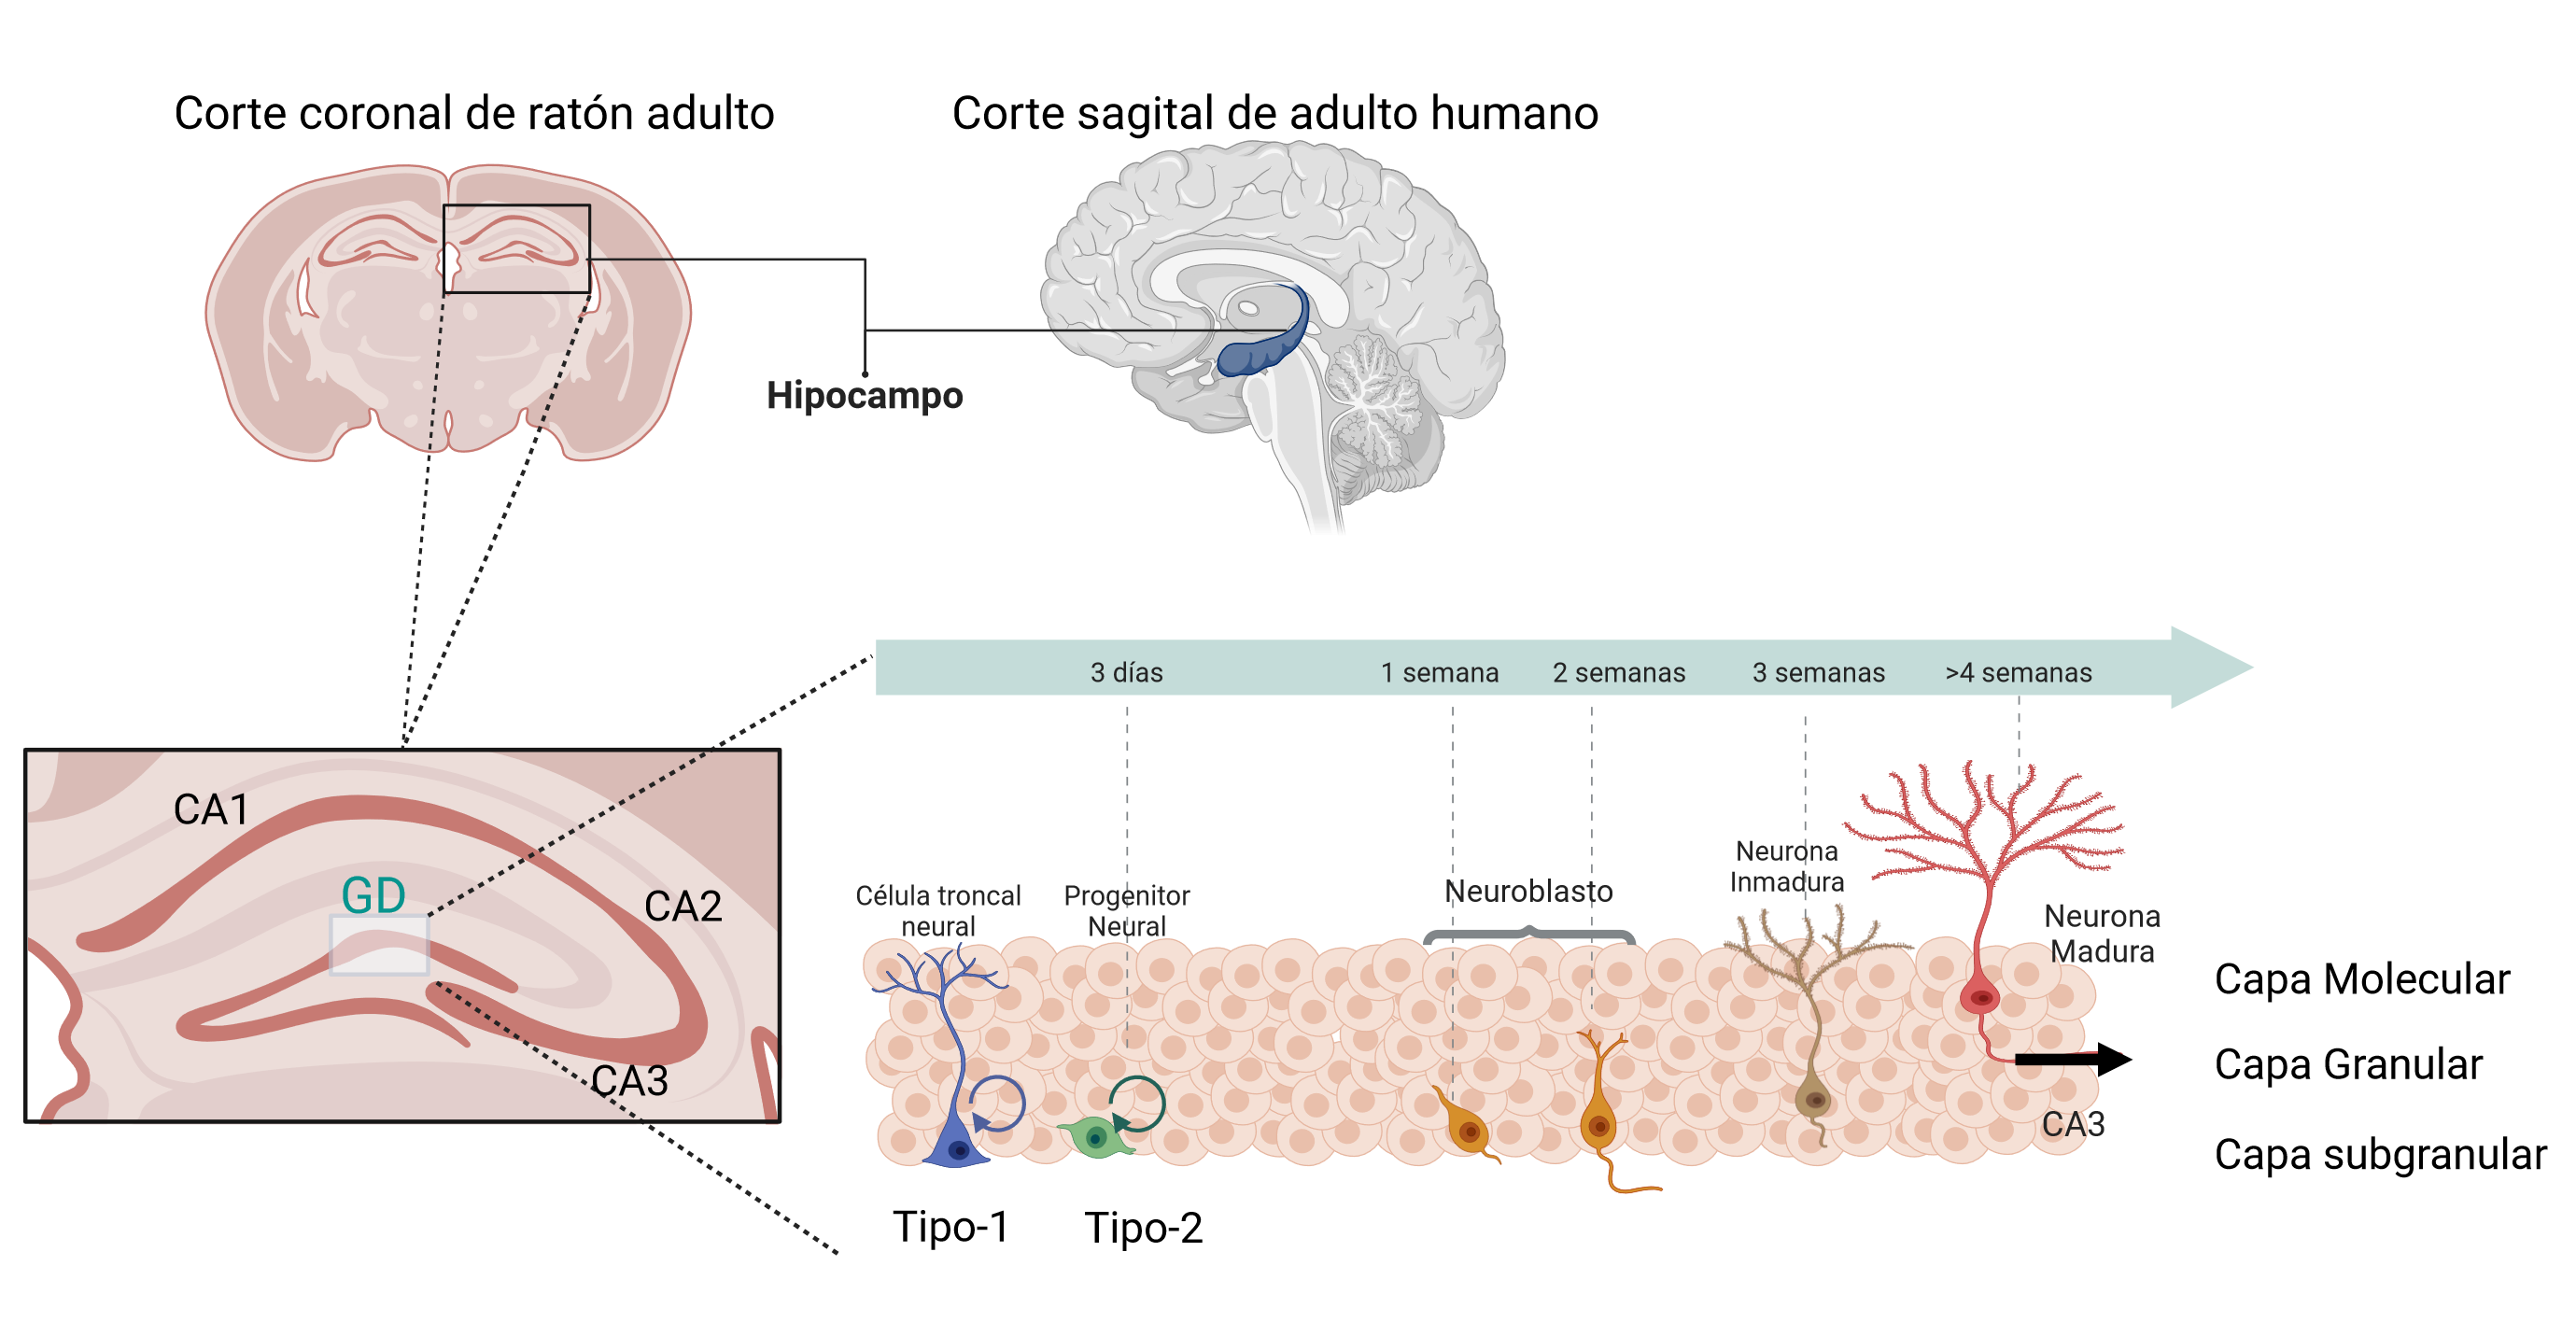
\includegraphics[width=0.85\linewidth,height=\textheight,keepaspectratio]{../Figures/neurogenesis_hipocampal.png}

}

\caption[Neurogénesis Adulta
hipocampal]{\label{fig-neurogenesishipo}Neurogénesis Adulta en el
\ac{gd}. La figura ilustra el proceso de \ac{nha}, mostrando las
diferentes etapas desde la célula troncal neural hasta la integración de
neuronas maduras en los circuitos neuronales. Este proceso se desarrolla
en un lapso de tiempo que abarca varias semanas. \emph{Etapas de la
Neurogénesis Adulta} {[}@batool2019; @denoth-lippuner2021{]}:
\textbf{Célula Troncal Neural o Célula de Tipo-1} (0-3 días): Estas
células, localizadas en la capa subgranular, tienen la capacidad de
proliferar y diferenciarse cuando reciben los estímulos adecuados, como
ejercicio aeróbico{[}@mustroph2012{]}. \textbf{Células Progenitoras
intermedias o progenitores neurales} (hasta los 7 días): Poseem una alta
capacidad proliferativa y se dividen varias veces aumentando la
población de células precursoras que eventualmente se convertirán en
neuronas. \textbf{Neuroblasto} (semana 1 a 2): Los progenitores neurales
se diferencian en neuroblastos, que comienzan a mostrar características
neuronales. \textbf{Migración} (semana 2 a 4): Los neuroblastos migran
hacia las capas granulares del \ac{gd} en el hipocampo. Durante esta
migración, los neuroblastos continúan madurando y establecen sus
primeras proyecciones a CA3. Durante las primeras tres semanas, la
mayoría de estas células mueren por apoptosis dependiente de BAX,
mientras que la \emph{supervivencia} es mediada por un mecanismo
dependiente de \ac{nmda}. \textbf{Maduración y Sinaptogénesis} (semana 4
a 8): Las nuevas neuronas continúan madurando, desarrollan un árbol
dendrítico más elaborado y aumentan la densidad de espinas dendríticas,
que son los sitios donde se forman las sinapsis excitatorias. En esta
etapa, las nuevas neuronas establecen conexiones más específicas y
fuertes con neuronas preexistentes, comenzando a participar en la
actividad sináptica del circuito (integración funcional). Información
tomada de @batool2019 y @denoth-lippuner2021}

\end{figure}%

Las principales teorías que abordan los roles cognitivos influenciados
por la \ac{nha} incluyen su papel en el aprendizaje y la recuperación de
la memoria. Estos fenómenos que se describen a continuación explican la
regulación de la memoria y la conducta desde diferentes enfoques
(@berdugo-vega2023) que pueden estar actuando de manera sinérgica
(@anacker2017).

\begin{tcolorbox}[enhanced jigsaw, colframe=quarto-callout-warning-color-frame, left=2mm, bottomrule=.15mm, rightrule=.15mm, arc=.35mm, toprule=.15mm, leftrule=.75mm, breakable, opacityback=0, colback=white]

\vspace{-3mm}\textbf{\textbf{NHA: mecanismos que modulan la conducta}}\vspace{3mm}

\textbf{Separación de Patrones} {[}@sahay2011{]}: Esta teoría destaca la
gran cantidad de células granulares en el \ac{gd} en comparación con las
neuronas en la \ac{ce} (una proporción de 5:1)
{[}@pattern\_chavlis\_2017{]}. El mayor número de células granulares
ayuda a crear grupos no superpuestos a partir de entradas similares
recibidas de la \ac{ce}, produciendo salidas que combinan información de
maneras significativas hacia CA3 sin interferir entre ellas. Esta
representación de memorias similares de forma
\href{AppendixB.qmd\#term-id-7}{ortogonal} (distintas) ayuda a
distinguir efectivamente patrones de entrada similares.

\begin{figure}[H]

\begin{minipage}{0.50\linewidth}

\begin{figure}[H]

\centering{

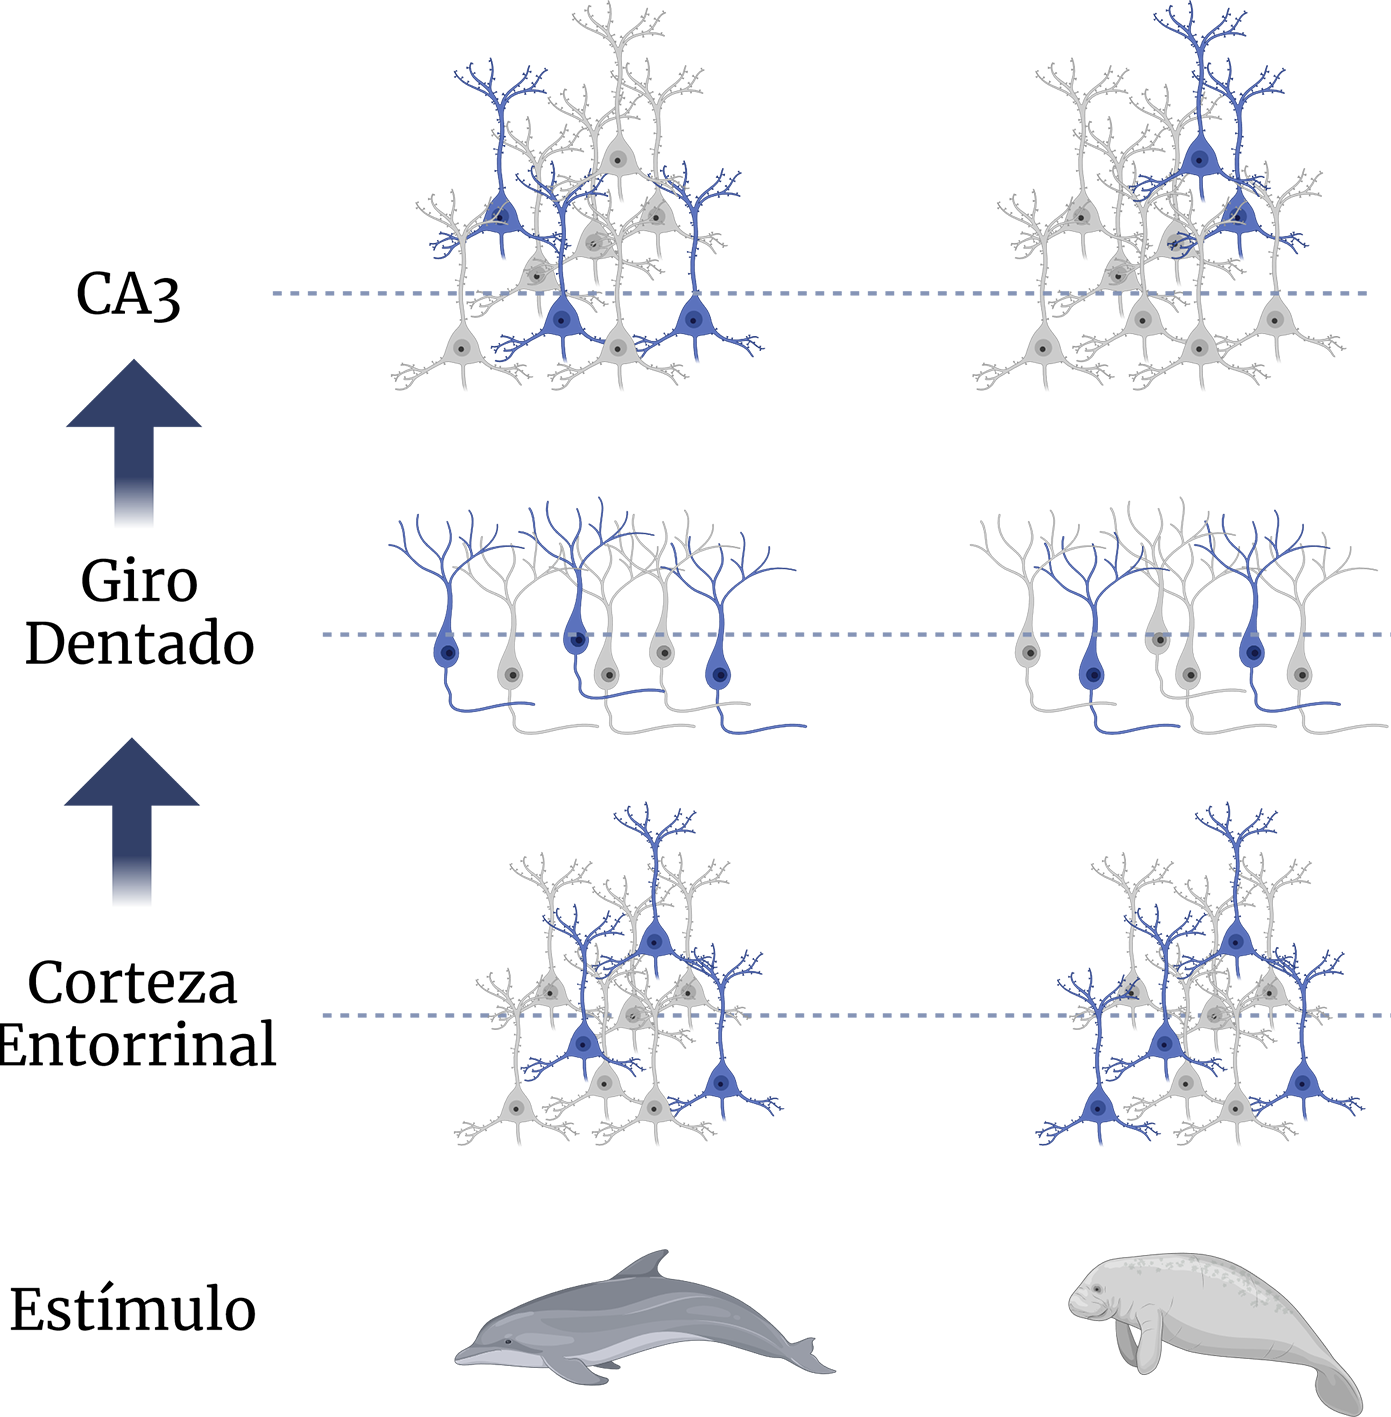
\includegraphics[width=0.9\linewidth,height=\textheight,keepaspectratio]{../Figures/neurogenesis_separacion_patrones.png}

}

\caption{\label{fig-separacionpatrones}Separación de patrones.}

\end{figure}%

\end{minipage}%
%
\begin{minipage}{0.05\linewidth}
~\end{minipage}%
%
\begin{minipage}{0.45\linewidth}
Durante la presentación de estimulos que generen patrones de actividad
similares en la \ac{ce}, la neurogénesis hipocampal permite reclutar
grupos no superpuestos de células granulares que a su vez activan
poblaciones distintas de células en CA3. El resultado la capacidad de
distinguir entre experiencias similares pero no idénticas. Ilustración
basada en @borzello2023\end{minipage}%

\end{figure}%

\textbf{Olvido y reaprendizaje} {[}@feng2001; @akers2014; @epp2016;
@adlaf2017{]}: La incorporación de nuevas neuronas puede remodelar las
redes neuronales existentes, potencialmente alterando o debilitando las
conexiones sinápticas previamente establecidas
(Figure~\ref{fig-olvido}). Este proceso puede interferir con las
memorias antiguas e inducir la ``limpieza'' de estas memorias a la vez
que facilita la adquisición de nuevas asociaciones (reaprendizaje). En
este caso, el olvido también previene la interferencia de memorias (al
igual que en la separación de patrones) {[}@olpe2023{]}, pero por otro
mecanismo con implicaciones distintas.

\begin{figure}[H]

\begin{minipage}{0.50\linewidth}

\begin{figure}[H]

\centering{

\pandocbounded{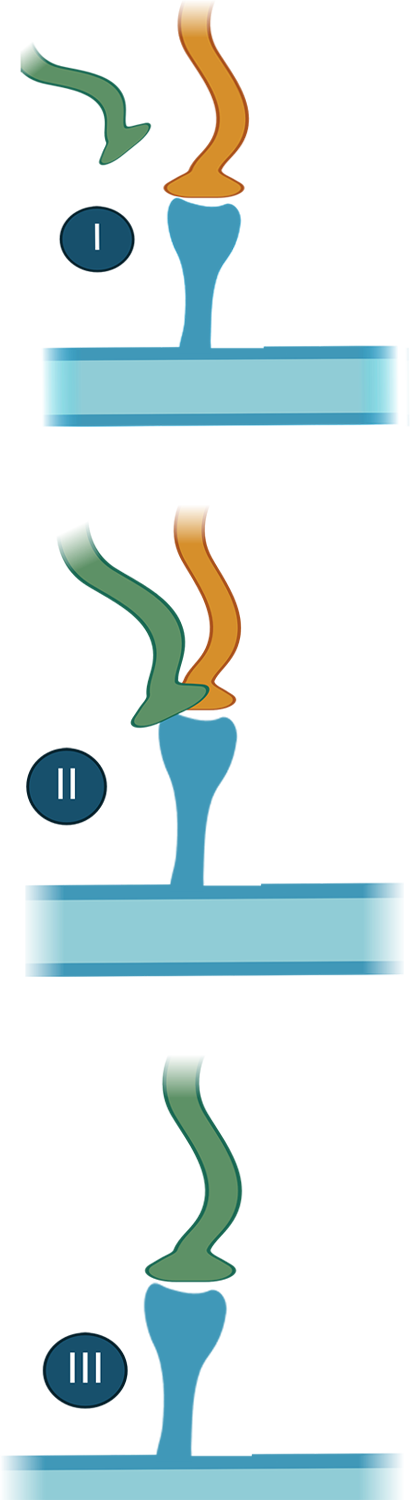
\includegraphics[keepaspectratio]{../Figures/neurogenesis_olvido.png}}

}

\caption{\label{fig-olvido}Desplazamiento de contactos sinápticos
previos por las terminales de nuevas neuronas.}

\end{figure}%

\end{minipage}%
%
\begin{minipage}{0.50\linewidth}
La integración de nuevas neuronas puede requerir ajustes en las sinapsis
existentes. En el primer panel, un axón de una nueva neurona (en
\textcolor{green}{verde}) es guiado por señales del medio (p.ej.
neurotrofinas) {[}@olpe2023 {]}. El cono de crecimiento es guiado por
proteínas asociadas a actina {[}@bailey2008{]} hasta alcanzar las
dendritas de CA3 aproximadamente dos semanas después de su nacimiento;
sin embargo, el contacto sináptico compienza hasta las 4 semanas (panel
II) {[}@toni2011;@toni2007{]}, donde el
\href{AppendixB.qmd\#term-id-52}{lamelopodio} se comienza a transformar
en una terminal presináptica vestigial que inicia el ensamblaje
sináptico mediado por CAMs (por sus siglas en inglés, \emph{Cell
Adhesion Molecules}). La integración de la nueva neurona modifica el
circuito previamente formado (en \textcolor{orange}{naranja}) (panel II)
y compite con éste (panel III) {[}@toni2015; @toni2015{]}, contribuyendo
posiblemente a fenómenos como el olvido al reemplazar el circuito
antiguo {[}@yau2015; @zhao2013{]}. Figura basada en los trabados de
@toni2015 y @toni2015\end{minipage}%

\end{figure}%

\textbf{Filtrado de información} {[}@borzello2023{]}: Esta teoría
propone que el \ac{gd} filtra patrones de entrada débiles o
inconsistentes, permitiendo que solo pasen patrones fuertes o
persistentes. Este evento es promovido por la capacidad de las neuronas
recién nacidas para mantener un tono inhibitorio en el \ac{gd}
(Figure~\ref{fig-inhibicion}) {[}@mcavoy2015; @mchugh2022{]}.

Uno de los aspectos más interesantes y cruciales de este proceso es que,
inicialmente, las nuevas neuronas son activadas predominantemente por el
neurotransmisor \ac{gaba} {[}@groisman2020{]}, que es típicamente
inhibitorio en neuronas maduras. En las neuronas inmaduras, hay una alta
concentración de iones de cloro dentro de la célula debido a la
actividad del cotransportador \(Na^+\) \(K^+\) \(Cl^-\) (nkcc1). Cuando
el \ac{gaba} se une a sus receptores (canales de cloro), en la neurona
nueva éste provoca una \emph{salida} de iones \(Cl^-\) de la célula, lo
que lleva a una \emph{despolarización} de la membrana y a la excitación
de la neurona. A medida que la neurona madura, ocurre un cambio en la
expresión de transportadores de cloro. El cotransportador \(K^+\)
\(Cl^-\) (kcc2) comienza a ser expresado en mayor medida, lo que reduce
la concentración de cloro intracelular. En esta etapa, la apertura de
los receptores \ac{gaba}érgicos permite la \emph{entrada} de iones de
cloro generando la hiperpolarización de la neurona. Por ende, antes de
las seis semanas, las neuronas recién nacidas se caracterizan por su
hiperexcitabilidad y alta plasticidad sináptica como consecuencia de la
inhibición reducida {[}@ge2007{]}. Sumado a esto, las nuevas neuronas
pueden inducir una inhibición lateral de neuronas granulares madulras
{[}@luna2019{]} (Figure~\ref{fig-inhibicion}).

Durante este período de 4-6 semanas, la actividad de la red del \ac{gd}
es generalmente inhibida por interneuronas que expresan parvalbúmina y
somatostatina, las cuales establecen conexiones con las células
granulares nuevas. La neurogénesis adulta produce una población neuronal
que permanece en gran medida apartada del tono inhibidor dominante en el
\ac{gd} y proporciona un canal de información paralelo para el
procesamiento de entradas no superpuestas {[}@groisman2020{]}.

\begin{figure}[H]

\centering{

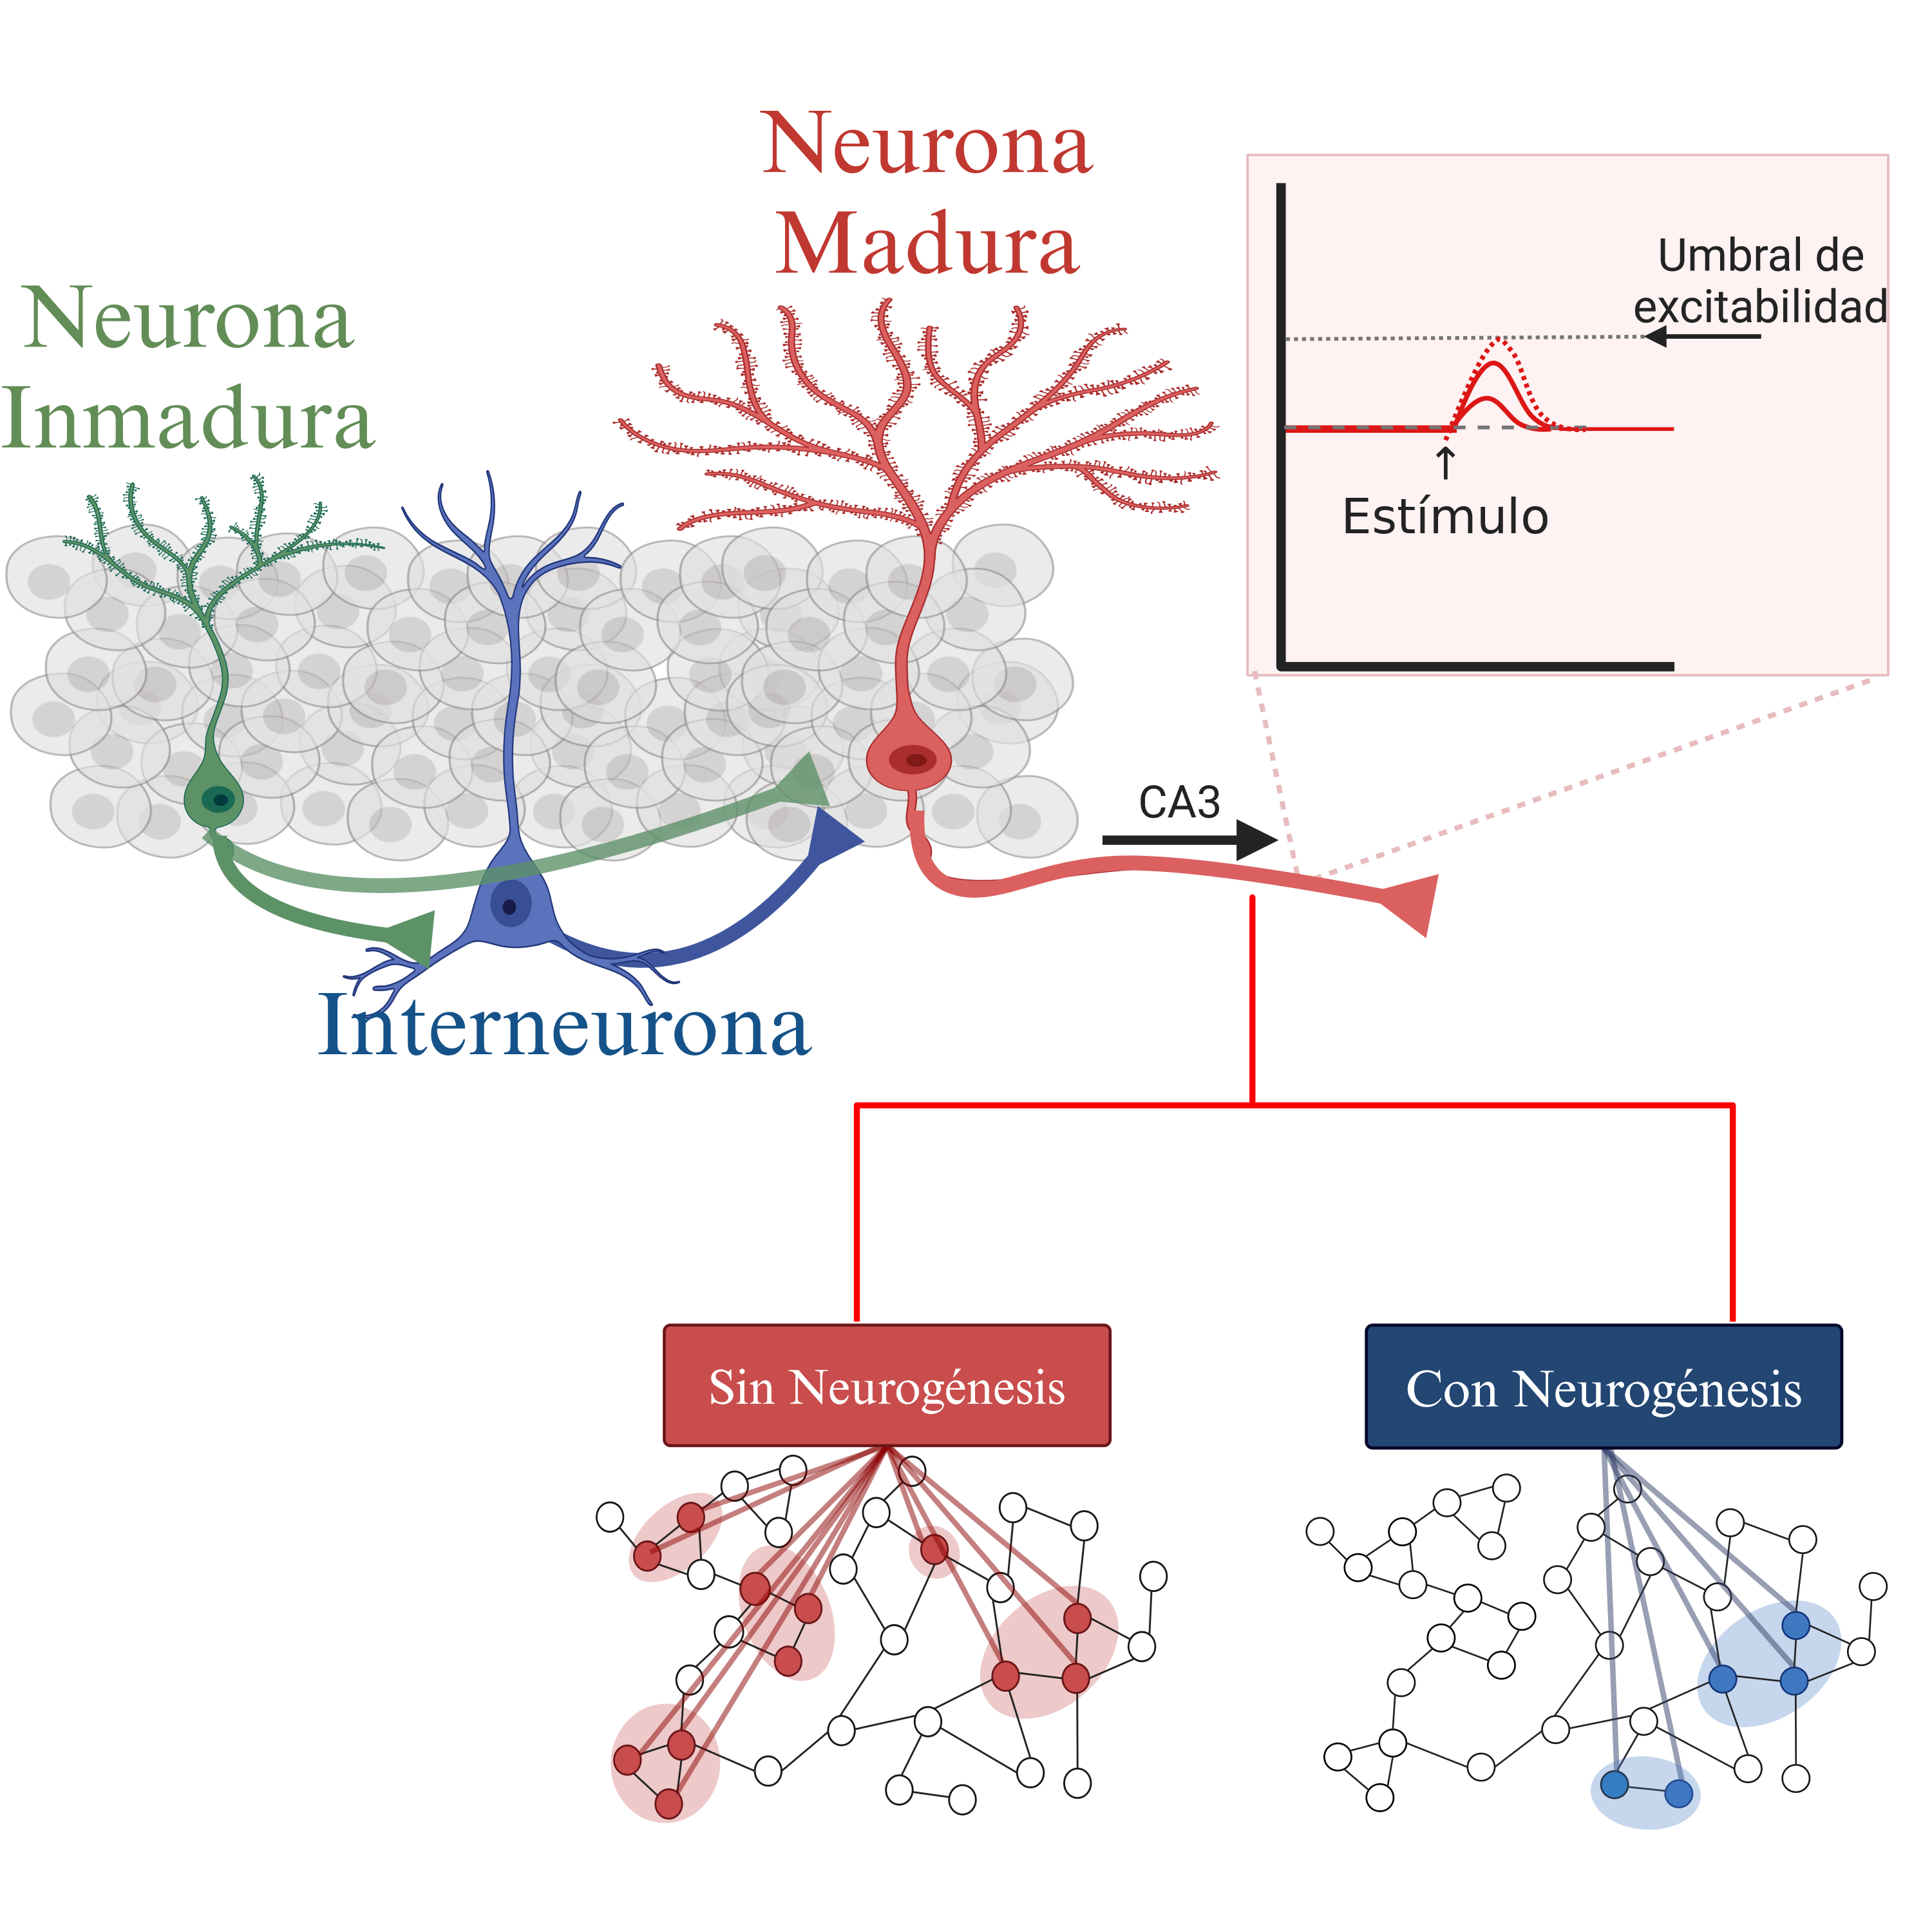
\includegraphics[width=0.8\linewidth,height=\textheight,keepaspectratio]{../Figures/neurogenesis_inhibicion.png}

}

\caption[Filtrado e inhibición en el
\ac{gd}]{\label{fig-inhibicion}Filtrado e inhibición. Teoría de filtrado
de información en el \ac{gd} y su relación con la \ac{nha}. La figura
ilustra cómo el GD filtra patrones de entrada débiles o inconsistentes,
lo que permite el paso sólamente de patrones fuertes o persistentes.
\emph{Neurona Inmadura}: Representada en verde, estas células recién
nacidas en el GD tienen una alta excitabilidad y juegan un papel crucial
en la modulación de la actividad del GD. \emph{Interneurona}:
Representada en azul, estas células son reclutadas por neuronas recién
nacidas y participan en la inhibición y filtrado de estímulos.
\emph{Neurona Madura}: Representada en rojo, estas células se integraron
al circuito maduro del \ac{gd} y proyectan hacia la región CA3 del
hipocampo participando en la transmisión de señales. El gráfico de
``Umbral de excitabilidad'' muestra cómo los estímulos deben superar un
umbral para generar una respuesta en el GD-CA3. La ausencia de nuevas
neuronas resulta en una hiperexcitabilidad en la región CA3, lo que
puede interferir con el reaprendizaje. Esta condición se ilustra con un
patrón rojo denso y desorganizado de conexiones sinápticas. La presencia
de nuevas neuronas aumenta la inhibición a través del reclutamiento de
interneuronas, lo que reduce la hiperexcitabilidad y permite un filtrado
efectivo de estímulos. Esto se representa con un patrón azul más claro y
organizado de conexiones sinápticas {[}@burghardt2012; @lacefield2012;
@luna2019{]}. Figura basada en el trabajo de @anacker2017}

\end{figure}%

\textbf{Detección de Novedad} {[}@vinogradova1975{]}: Las nuevas
neuronas muestran una mayor actividad durante experiencias nuevas o
cambiantes, promoviendo el reclutamiento de diferentes grupos celulares
cuando se introducen nuevos estímulos. Este fenómeno está relacionado
con las propiedades de las neuronas recién nacidas en el \ac{gd} del
hipocampo, que poseen alta plasticidad y son especialmente sensibles a
nuevas experiencias {[}@borzello2023{]}. Como señalan @groisman2020, las
células granulares recién nacidas en el hipocampo muestran una alta
excitabilidad y un umbral bajo para inducir procesos de plasticidad,
como LTP, durante las primeras 4-6 semanas después de su nacimiento.

\textbf{Indexación y Etiquetado Temporal} {[}@teyler1986; @manns2007{]}:
Estas teorías proponen que la mayor excitabilidad del \ac{gd} se debe al
reclutamiento continuo de células granulares recién nacidas y altamente
excitables a lo largo del tiempo. Esta incorporación continua de células
adultas permite al \ac{gd} codificar índices únicos (p.~ej.,
\href{AppendixB.qmd\#term-id-1}{engramas}) para memorias que se
almacenan de manera cronológica, facilitando la distinción secuencial de
eventos temporales.

\end{tcolorbox}

\begin{tcolorbox}[enhanced jigsaw, colframe=quarto-callout-important-color-frame, left=2mm, bottomrule=.15mm, rightrule=.15mm, arc=.35mm, toprule=.15mm, leftrule=.75mm, breakable, opacityback=0, colback=white]

\vspace{-3mm}\textbf{\textbf{Estudio de la NHA en modelos animales e implicaciones sobre la
flexibilidad cognitiva}}\vspace{3mm}

Varias líneas de investigación {[}@anacker2017{]} señalan que la
\ac{nha} es esencial para la
\href{@AppendixB.qmd\#term-id-19}{flexibilidad cognitiva}, la cual
permite la adaptación de pensamientos y conductas a nuevas situaciones
{[}@cognitive\_uddin\_2021{]} mediante la formación y recuperación de
recuerdos contextuales y espaciales {[}@okeefe1990{]}, así como la
integración de nueva información con experiencias pasadas
(Figure~\ref{fig-flexneuro}) {[}@epp2016; @martinez-canabal2019;
@scott2021{]}. Por otro lado, las alteraciones en la NHA disminuyen la
flexibilidad cognitiva {[}@garthe2016; @epp2016{]}, como se observa en
trastornos depresivos y de ansiedad {[}@cognitive\_uddin\_2021{]}.

El estudio de la flexibilidad cognitiva en el aprendizaje y la memoria
espacial en modelos animales proviene del desarrllo de experimentos en
laberintos que datan de principios del siglo XX {[}@goodman2024{]}.
@small1900 inició la experimentación en laberintos comparando las
habilidades mentales de ratas salvajes y domesticadas, registrando el
tiempo y errores cometidos al resolver el laberinto. A partir de este
trabajo pionero, se realizaron cada vez más protocolos conductuales en
distintos laberintos tanto terrestres, como acuáticos
{[}@vorhees2006{]}. En general, se distinguen dos fases importantes en
el aprendizaje en los laberintos {[}@othman2022{]}: una fase de
\emph{descubrimiento}, donde el animal aprende a recorrer el laberinto
para obtener una recompensa, y una fase que implica mejorar la
resolución del laberinto, cada vez con menos errores {[}@tolman1927{]},
un indicador de aprendizaje.

Un laberinto que sigue siendo clave para entender los distintos aspectos
de la memoria (consolidación, retención, evocación, reconsolidación) es
el \textbf{\ac{mwm}} {[}@morris1981{]}. Entre sus múltples protocolos,
permite el estudio de memorias dependientes del hipocampo (p.ej. memoria
espacial) {[}@hernandez-mercado2022{]} y evaluar la importancia de la
neurogénesis hipocampal en la conducta {[}@vanpraag1999;
@garthe2013{]}. El hecho de que diferentes lesiones
\colorbox{BurntOrange}{o alteraciones a la dinámica hipocampal}
{[}@developments\_morris\_1984{]}, como las inducidas por el estrés
crónico {[}@dhooge2001; @vorhees2006{]}, afecten el rendimiento en este
laberinto resalta su importancia y su relevancia en establecer la
relación entre la neurogénesis hipocampal y la flexibilidad cognitiva,
como se ejemplifica en la Figure~\ref{fig-flexneuro}.

\begin{figure}[H]

\centering{

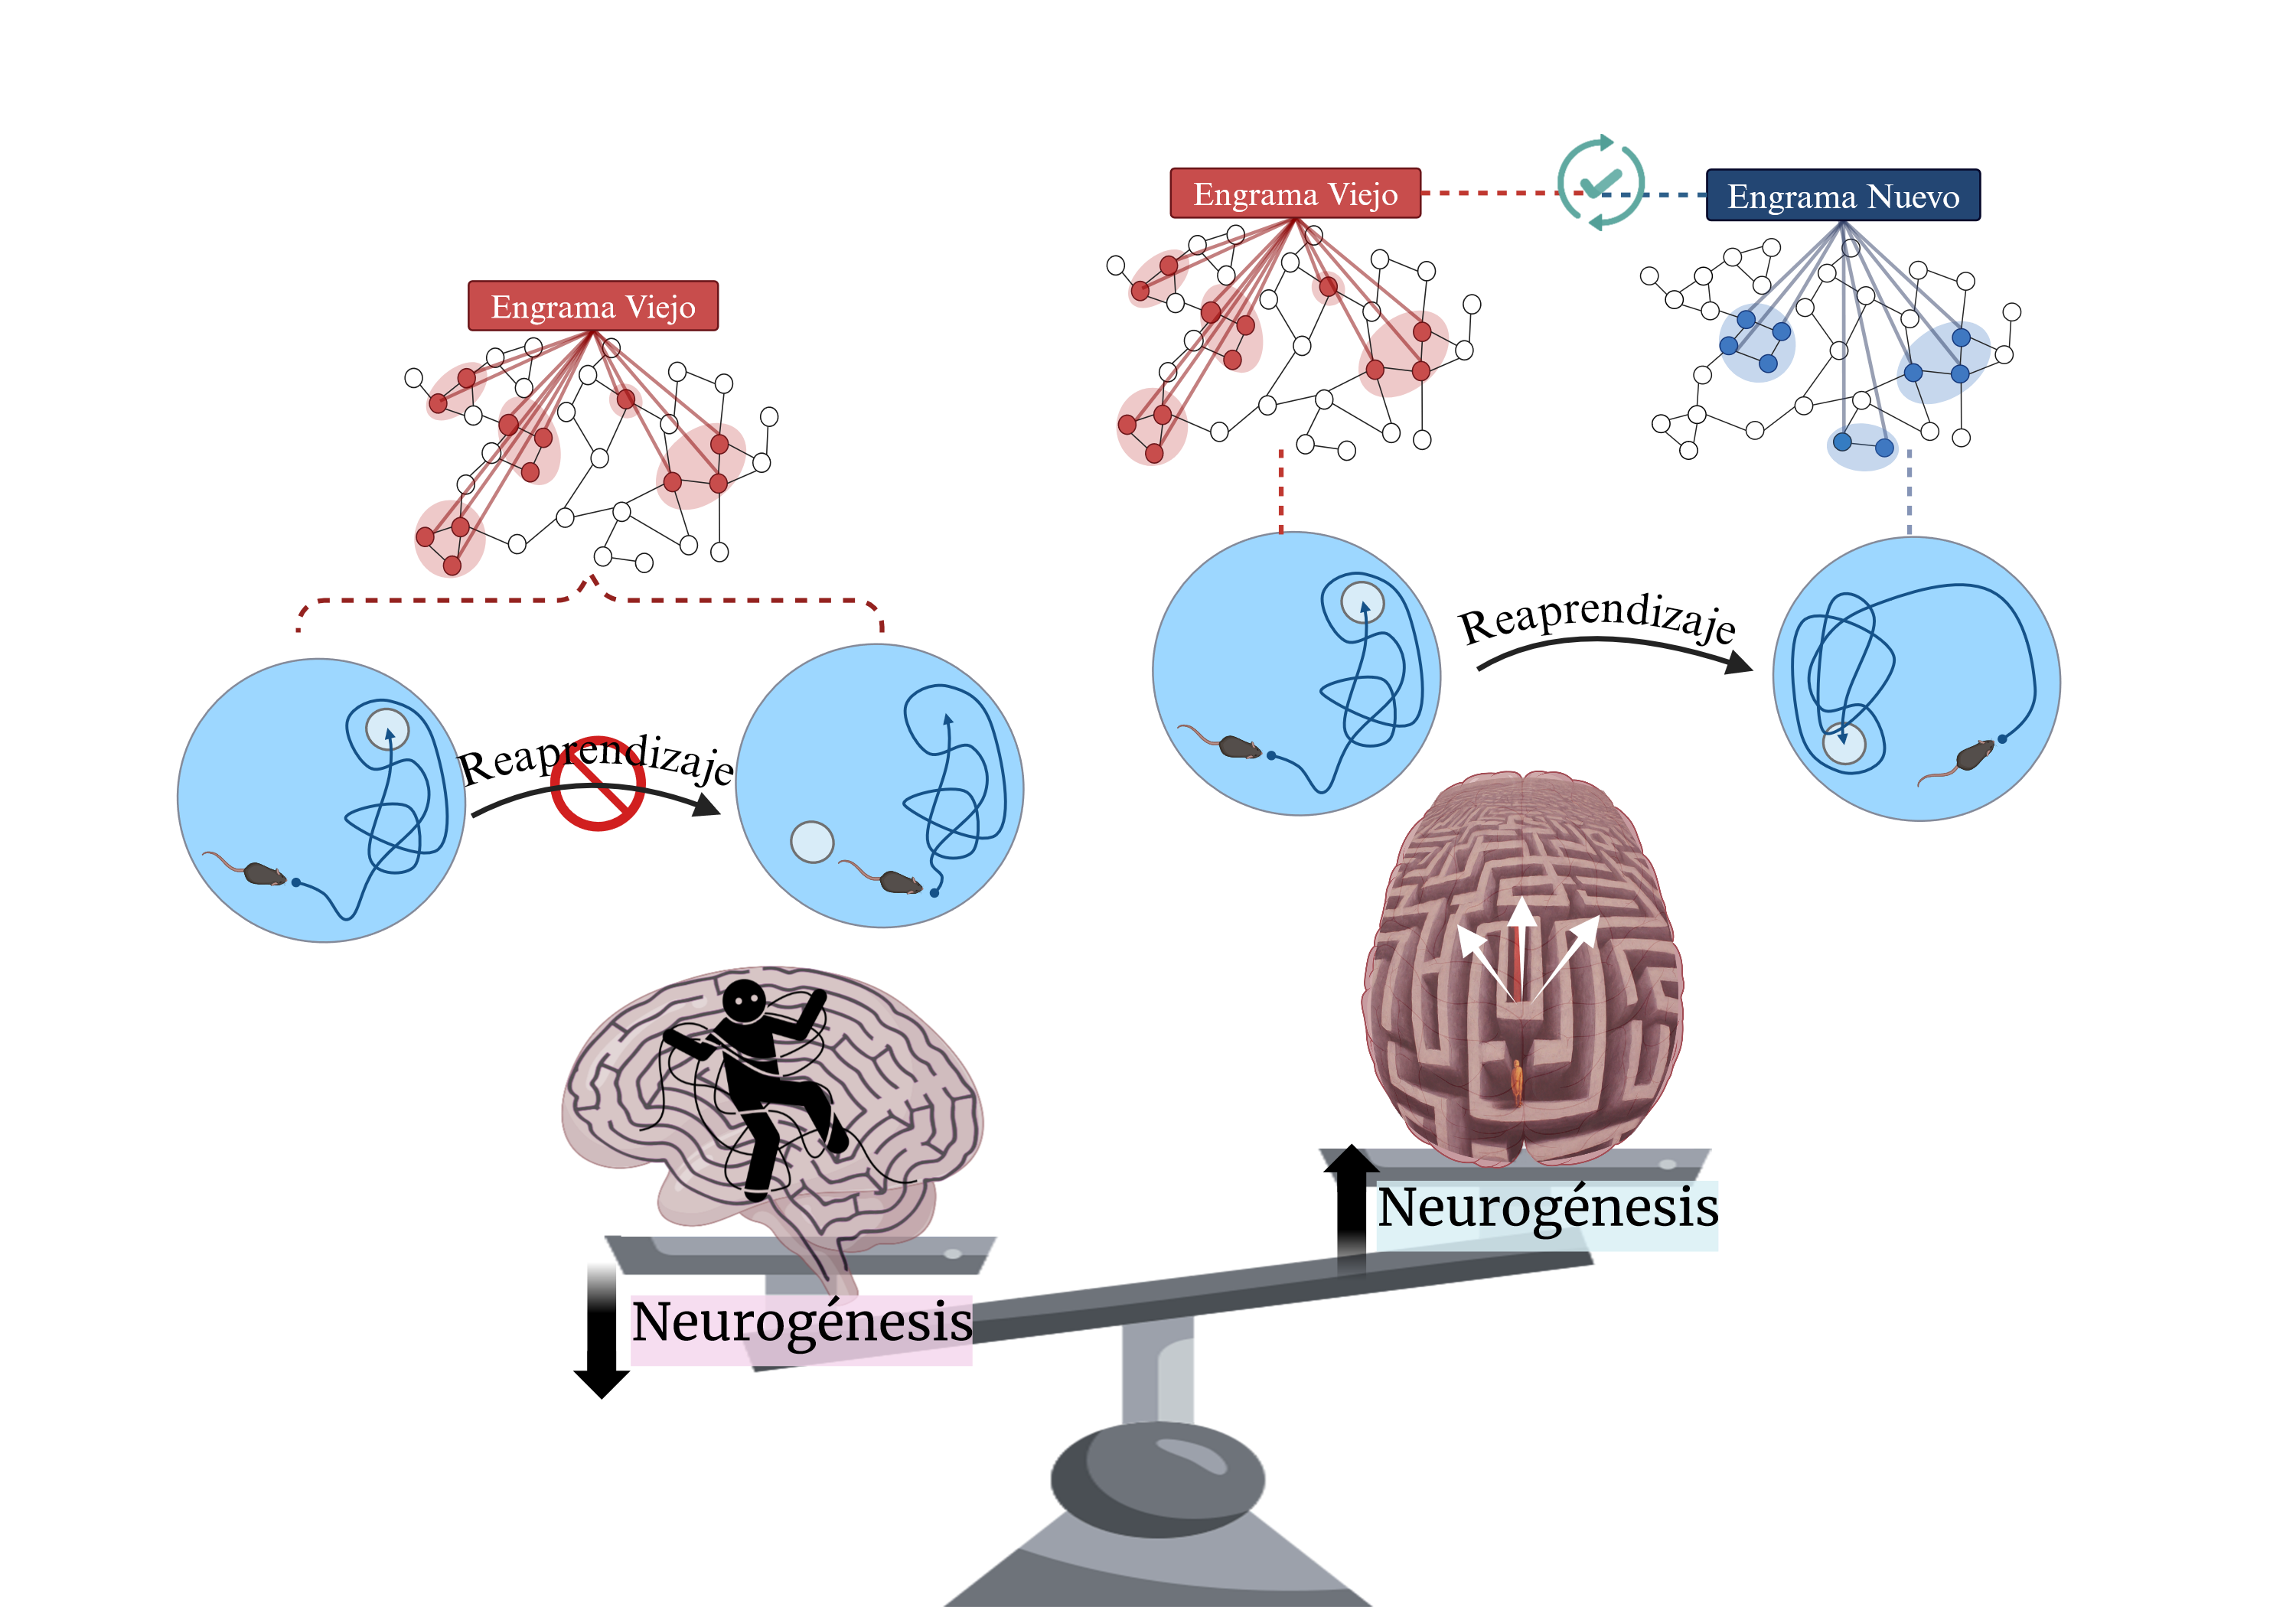
\includegraphics[width=0.75\linewidth,height=\textheight,keepaspectratio]{../Figures/flexibilidad_balanza.png}

}

\caption[Neurogénesis y Flexibilidad en la
Memoria]{\label{fig-flexneuro}Neurogénesis hipocampal como facilitador
de la flexibilidad en la memoria. La figura ilustra cómo la neurogénesis
en el hipocampo actúa como un mecanismo que facilita la flexibilidad de
la memoria, permitiendo el reaprendizaje y la adaptación a nuevas
situaciones. Se presenta un balance entre la neurogénesis y el
mantenimiento de memorias antiguas, destacando su impacto en el
reaprendizaje de tareas como la prueba del \ac{mwm}. \emph{Parte
Izquierda (Neurogénesis Reducida)}: Engramas Viejos, representados en
rojo, muestran conexiones sinápticas persistentes que dificultan el
olvido de memorias antiguas. Impedimento del Reaprendizaje: La reducción
en la neurogénesis limita la capacidad de olvidar memorias viejas, lo
que a su vez obstaculiza el aprendizaje de nuevas tareas. Este proceso
es visualizado mediante la incapacidad de la figura para navegar
eficazmente en el laberinto. \emph{Parte Derecha (Aumento de la
Neurogénesis)}: La figura muestra cómo el aumento de la neurogénesis
facilita el olvido de memorias viejas (engramas en rojo) y la formación
de nuevas memorias (engramas en azul). Facilitación del Reaprendizaje.
Un aumento en la neurogénesis permite el olvido de engramas viejos, lo
que facilita el reaprendizaje y la adquisición de nuevas habilidades y
conocimientos. Este proceso es visualizado mediante la figura navegando
exitosamente en el laberinto. Basado en la figura 2 de @anacker2017.}

\end{figure}%

La relación entre la \ac{nha} y la flexibilidad cognitiva se vuelve
especialmente relevante cuando se considera su implicación en trastornos
como la ansiedad y la depresión. Las personas con ansiedad y depresión
tienden a experimentar pensamientos negativos recurrentes
(\href{AppendixB.qmd\#term-id-70}{rumiaciones}) y/o a generalizar
experiencias (ansiedad) (Figure~\ref{fig-flexibilidad})
{[}@denoth-lippuner2021{]}, manifestaciones de falta de flexibilidad
cognitiva. Esta falta de flexibilidad dificulta la capacidad para
desvincularse de estos pensamientos negativos, prolongando y exacerbando
el malestar emocional {[}@guler2022{]}.

\begin{figure}[H]

\begin{minipage}{0.60\linewidth}
\textcolor{darkgray}{La figura presenta un laberinto metafórico que ilustra cómo la flexibilidad cognitiva permite la adaptación al ambiente, la resolución de problemas y el reaprendizaje}
{[}@anacker2017; @waltz2017; @doss2021{]},
\textcolor{darkgray}{mientras que la falta de flexibilidad cognitiva conduce a pensamientos obsesivos, rumiaciones e ideas fijas, asociándose con síntomas depresivos y ansiosos}
{[}@garthe2016; @jett2017{]}. \emph{Flexibilidad Cognitiva (camino
azul)}:
\textcolor{darkgray}{La flexibilidad cognitiva permite la adaptación a cambios y nuevas circunstancias. Además, facilita la generación de nuevas estrategias para enfrentar desafíos y promueve la capacidad para resolver problemas de manera efectiva. Como consecuencia, favorece el aprendizaje de nuevas habilidades y conocimientos. *Falta de Flexibilidad Cognitiva (camino rojo)*: Esto se asocia con pensamientos repetitivos y obsesivos que dificultan la resolución de problemas, fijación en ciertos pensamientos  (rumiaciones) o ideas que impiden el progreso (obsesiones) y rigidez en el pensamiento que impide la adaptación y el cambio. Como consecuencia, se mantiene al individuo atrapado en un estado de frustración y malestar}.
Basado en las ideas de @guler2022 y
@cognitive\_uddin\_2021.\end{minipage}%
%
\begin{minipage}{0.40\linewidth}

\begin{figure}[H]

\centering{

\pandocbounded{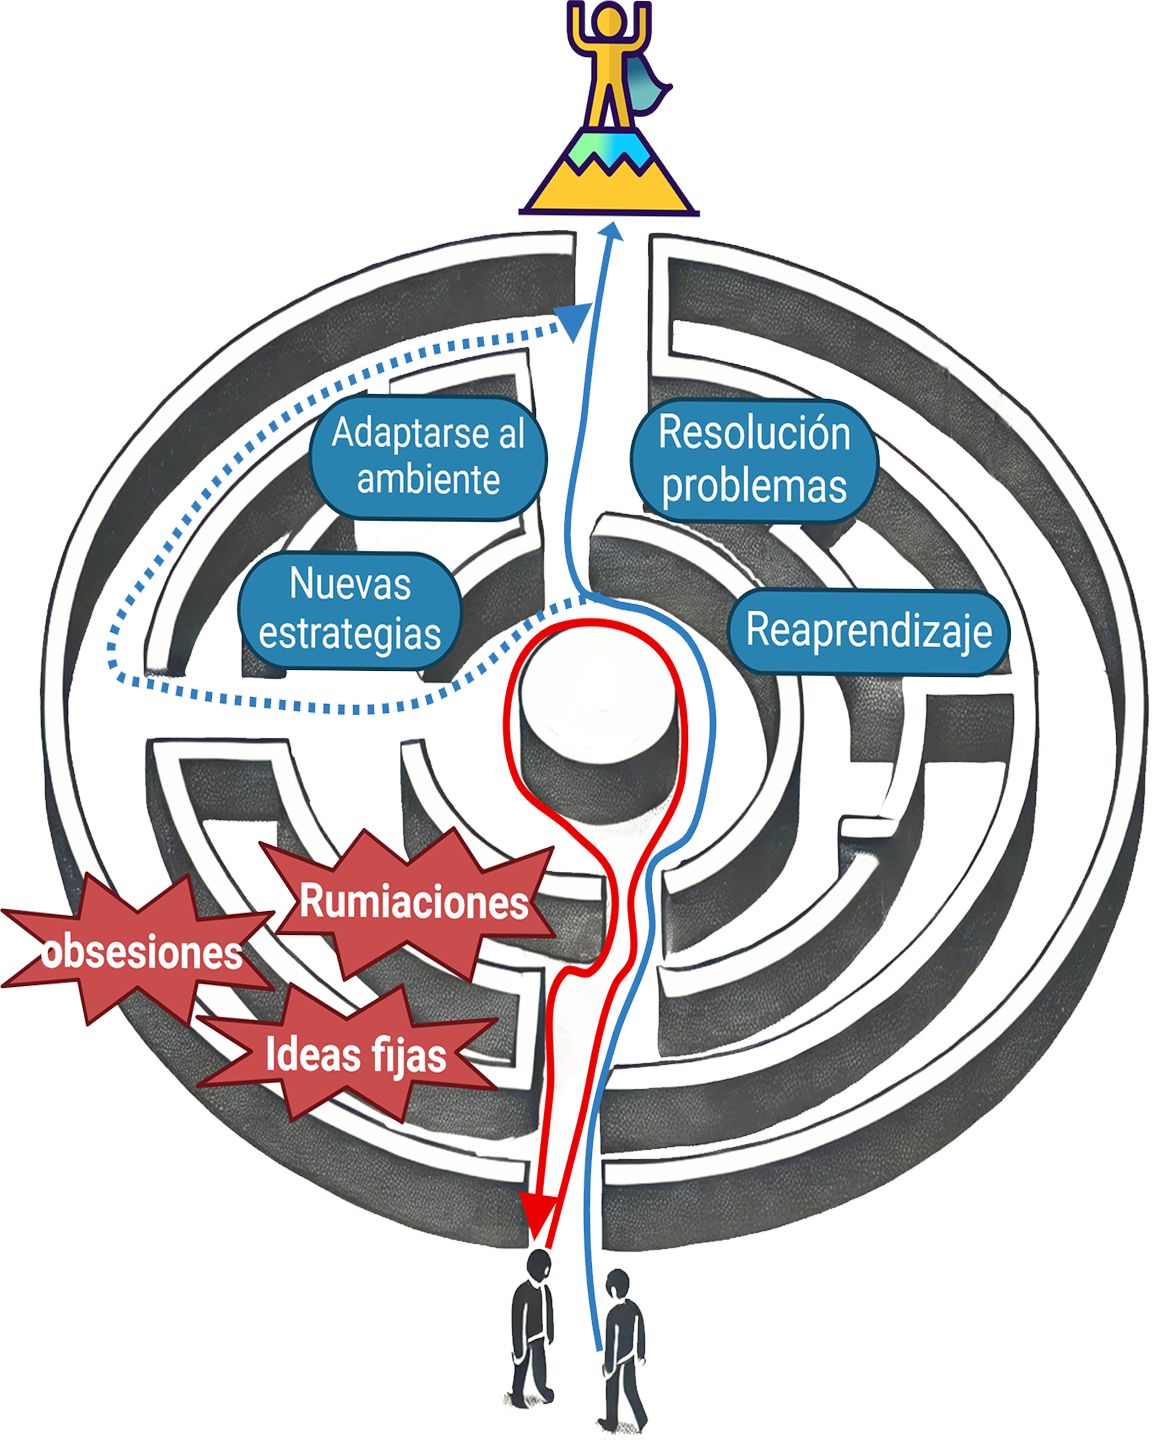
\includegraphics[keepaspectratio]{../Figures/flexibilidad_cognitiva.png}}

}

\caption{\label{fig-flexibilidad}Flexibilidad cognitiva y trastornos
mentales.}

\end{figure}%

\end{minipage}%

\end{figure}%

Sin embargo, como se resaltan en numerosas investigaciones
{[}@young2009; @young2021; @maei2009a; @garthe2013;
@hernandez-mercado2022{]}, estudios sobre la función cognitiva en
modelos de roedores utilizando el \ac{mwm} ha dependido
predominantemente del análisis de métricas subóptimas que no modelan los
procesos cognitivos que se quieren representar. Si bien estos métodos
han proporcionado valiosos conocimientos, existen novedosos enfoques que
pueden proporcionar interpretaciones más matizadas de los datos y el
impacto de la NHA sobre la flexibilidad. Debido a que la interpretación
de los datos obtenidos en el MWM es crucial para el entendimiento de los
impactos cognitivos que tiene el estrés crónico, se debe tener en cuenta
esto y utilizar métricas y análisis adecuados.

\end{tcolorbox}

\subsection{Estrés y Cognición}\label{estruxe9s-y-cogniciuxf3n}

@lazarus2006 define el estrés como la reacción interna del cuerpo ante
cualquier estímulo externo que se considere no placentero o dañino. Como
señala Lazarus en su libro, cada individuo experimenta y afronta los
estímulos aversivos de manera diferente. Estas diferencias están
influenciadas por factores psicológicos, biológicos y ambientales
{[}@tafet2016{]}. No obstante, en presencia de estresores crónicos,
impredecibles e incontrolables, la capacidad fisiológica para enfrentar
estos estímulos puede verse superada, contribuyendo así al desarrollo de
trastornos mentales, como los trastornos depresivos o de ansiedad
{[}@hill2012{]}.

A nivel cognitivo, los efectos del estrés crónico incluyen dificultad en
la formación de memorias episódicas y dificultades para adaptar
pensamientos y conductas de forma flexible {[}@sandi2013{]}. A nivel
emocional, estas alteraciones cognitivas contribuyen y mantienen los
síntomas de estrés y ansiedad que dificultan la recuperación del
individuo {[}@anacker2017{]}. Estas alteraciones están íntimamente
relacionadas con los efectos que el estrés crónico tiene sobre la
formación hipocampal {[}@el-aziz2022{]}.

\subsubsection{Respuesta de la formación hipocampal al
estrés}\label{respuesta-de-la-formaciuxf3n-hipocampal-al-estruxe9s}

La formación hipocampal es una estructura particularmente sensible al
estrés crónico {[}@cobb2013{]}. Hace casi tres décadas, @sheline1996
examinaron los cambios en el volumen del hipocampo en pacientes con
trastorno depresivo mayor utilizando resonancia magnética y encontraron
una reducción del 12\%--16\% en el volumen del hipocampo en ambos
hemisferios. En otro estudio, @steffens2000 incluyeron a pacientes
geriátricos \colorbox{BurntOrange}{con depresión} y confirmaron una
reducción del 4\%--7\% en el volumen del hipocampo en comparación con
los controles sin diagnóstico depresivo. Más recientemente,
@treadway2015 reportaron una reducción del volumen del hipocampo en
pacientes con trastorno depresivo mayor y una correlación inversa entre
el número de episodios depresivos y el volumen del \ac{gd}.

El mecanismo principal que parece inducir estos cambios estructurales
está relacionado con los niveles elevados de glucocorticoides en
respuesta al estrés crónico {[}@conrad2008{]}. Estos pueden generar
atrofia de dendritas en \ac{ca}3 {[}@fuchs1998{]} y \ac{gd}
{[}@bessa2009{]}, así como una reducción de la \ac{nha} {[}@hill2015{]}.
En conjunto, estos daños se observan en los hipocampos con menores
volúmenes en pacientes que experimentan constantemente estrés crónico y
cuadros depresivos {[}@anand2012{]}. Este mecanismo inicia con la
activación del eje \ac{hpa}, responsable de la liberación de
\href{AppendixB.qmd\#term-id-32}{glucocorticoides}. Cuando enfrentamos
un estresor, el hipotálamo secreta \ac{crh}, que a su vez hace que la
glándula pituitaria anterior libere \ac{acth} (Figure~\ref{fig-HPA}). La
\ac{acth} viaja a través del torrente sanguíneo hasta las glándulas
suprarrenales, donde fomenta la liberación de \emph{glucocorticoides},
principalmente \emph{cortisol} en los humanos. El \emph{cortisol} luego
envía señales al hipotálamo y la pituitaria para detener la liberación
de \ac{crh} y \ac{acth}, regulando así la actividad de este eje \ac{hpa}
{[}@silverman2012{]}. Sin embargo, el estrés crónico puede alterar esta
regulación y generar niveles constantemente altos de \emph{cortisol}
asociados al desarrollo de distintas patologías {[}@sandi2013;
@hurtubise2017{]}.

\begin{figure}

\centering{

\pandocbounded{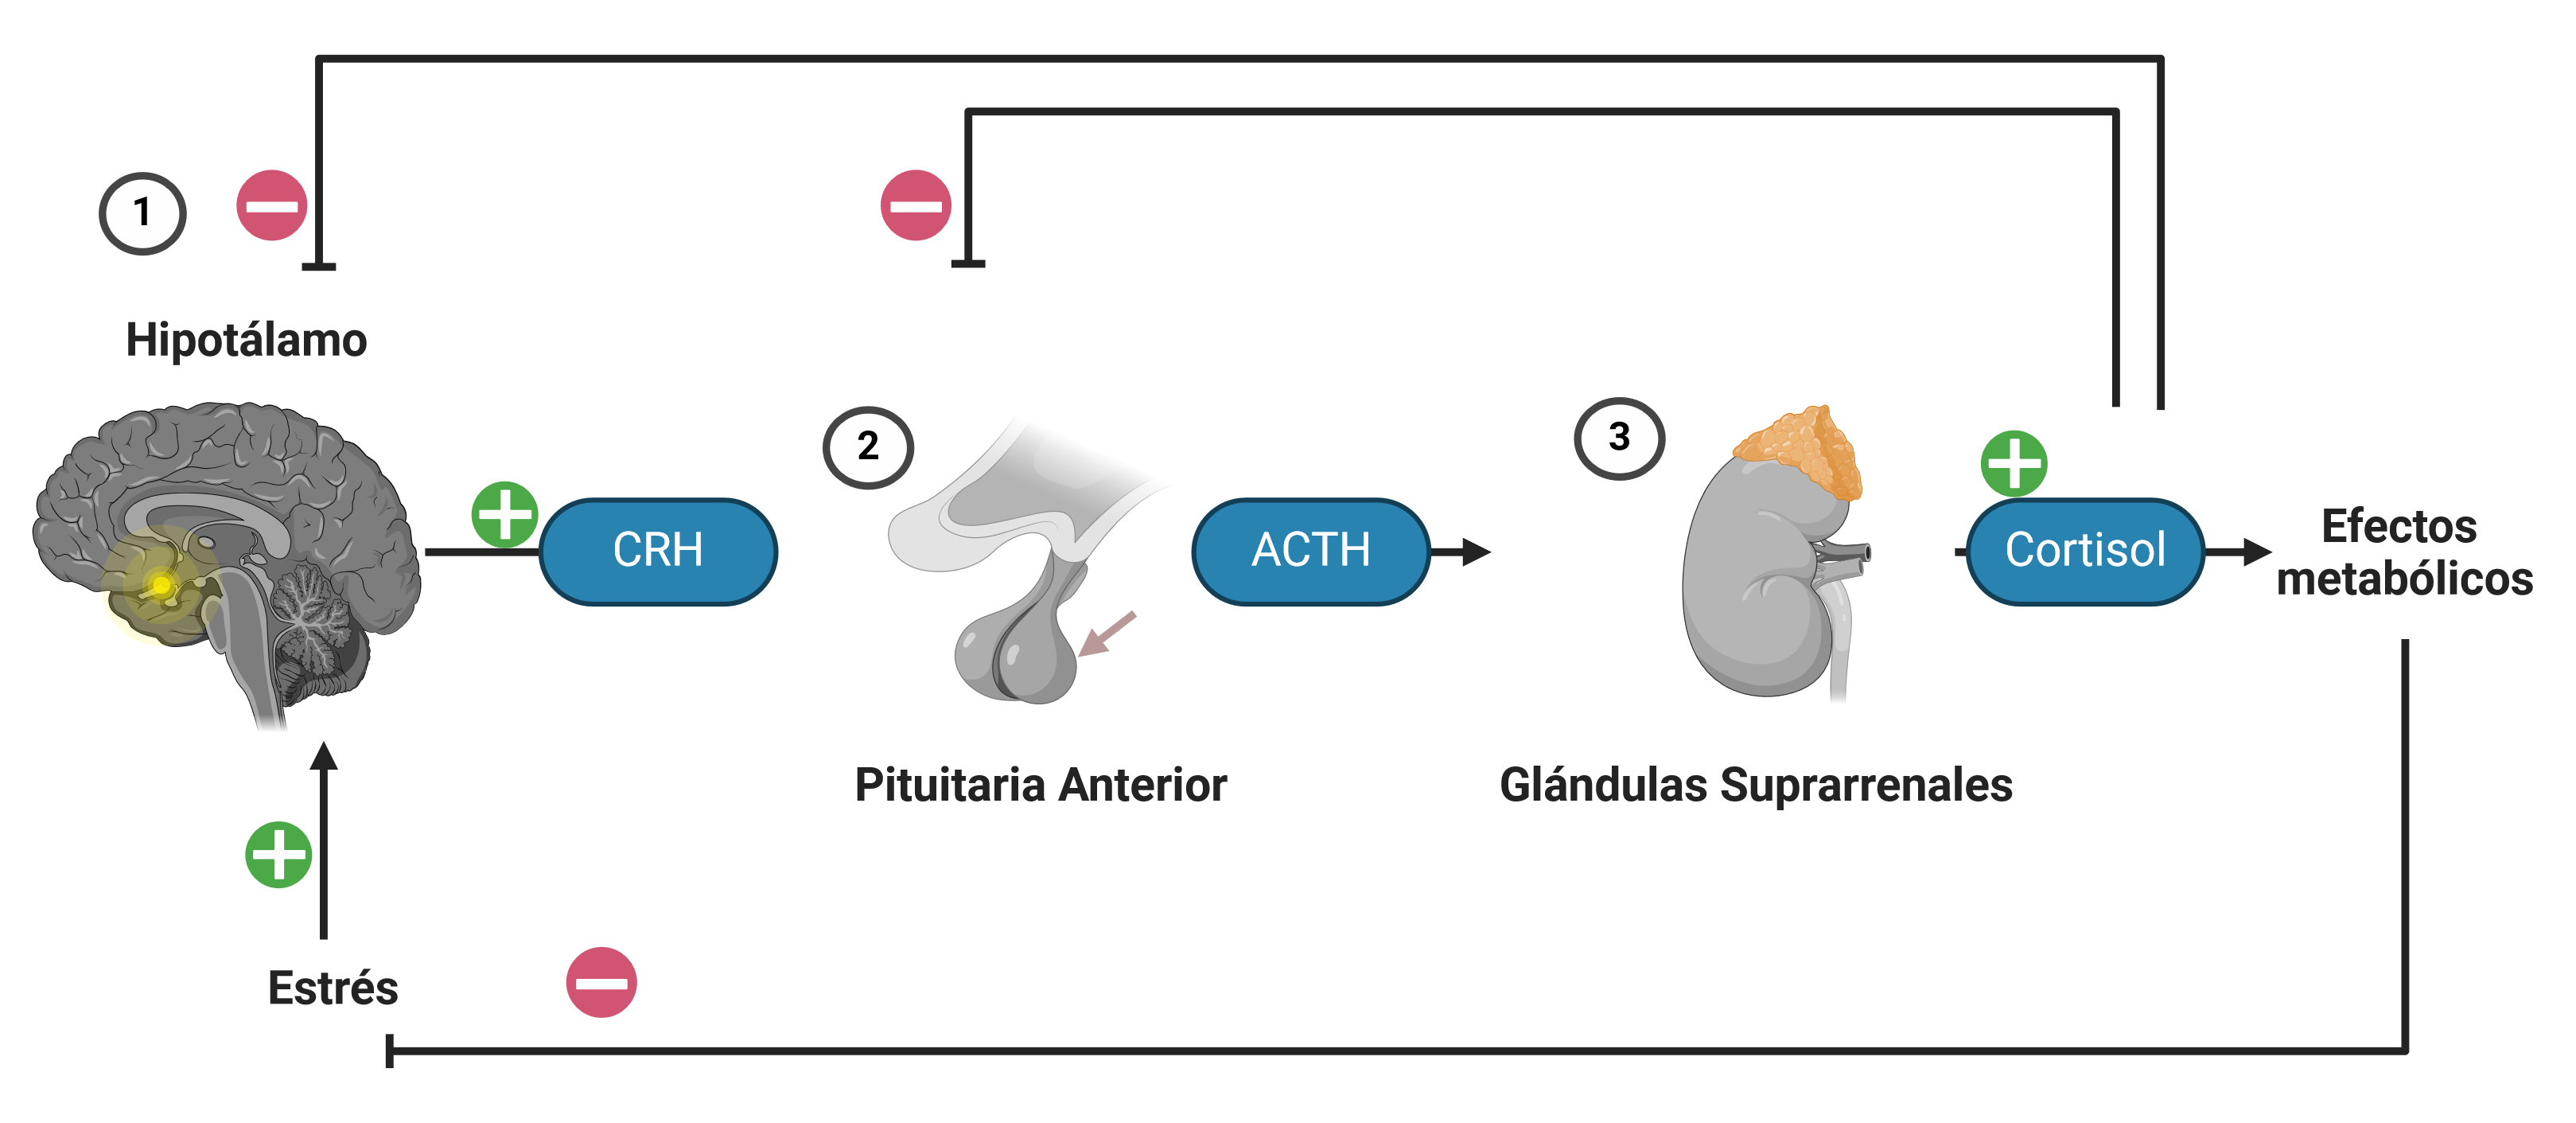
\includegraphics[keepaspectratio]{../Figures/HPA_long.png}}

}

\caption[Regulación del Eje HPA en respuesta al
estrés]{\label{fig-HPA}Regulación del Eje \ac{hpa} en respuesta al
estrés. El proceso comienza en el hipotálamo (1), que en respuesta a
señales de estrés, secreta \ac{crh}. La \ac{crh} actúa sobre la
pituitaria anterior (2), estimulando la liberación de \ac{acth} en el
torrente sanguíneo. La \ac{acth}, a su vez, actúa sobre las glándulas
suprarrenales (3), promoviendo la secreción de cortisol
{[}@silverman2012{]}. El sistema de retroalimentación negativa está
representado por las señales de inhibición (indicadas por los símbolos
negativos rojos), donde niveles elevados de cortisol inhiben tanto la
secreción de \ac{crh} en el hipotálamo como la secreción de \ac{acth} en
la pituitaria anterior, ayudando a mantener la homeostasis y evitar una
respuesta excesiva al estrés {[}@dealcubierre2023{]}. Las flechas verdes
con el signo positivo indican la activación de cada componente del eje
\ac{hpa}. Información tomada de @silverman2012}

\end{figure}%

Es importante señalar que las alteraciones en la regulación del eje
\ac{hpa} no solo afectan a la liberación de cortisol, sino que también
tienen implicaciones significativas en otras áreas del cerebro, como las
\href{AppendixB.qmd\#term-id-49}{células granulares} del \ac{gd}. Estas
células granulares son de las pocas neuronas que expresan tanto
receptores de \emph{mineralocorticoides} (p.~ej. \emph{aldosterona})
como de \emph{glucocorticoides} (p.~ej. \emph{cortisol})
{[}@reul1985{]}. Por lo tanto, no es sorprendente que las células
granulares sean especialmente susceptibles al daño por niveles elevados
de hormonas suprarrenales {[}@boldrini2012{]}. Adicionalmente, las
hormonas que se secretan en respuesta al estrés también tienen un
impacto profundo en la regulación de varios neurotransmisores en el
cerebro, incluyendo la \ac{5-ht} {[}@alenina2015{]}, un neurotransmisor
crucial involucrado en la regulación del estado de ánimo
{[}@serotonin\_mudzka\_2018{]}.

\subsubsection{Sistema
serotoninérgico}\label{sistema-serotoninuxe9rgico}

La mayoría de las neuronas serotoninérgicas en el sistema nervioso se
encuentran dentro de los límites de los ``\emph{núcleos del rafé}''
{[}@tafet2016{]}. Estos núcleos se pueden clasificar, basándose en su
distribución y proyecciones principales, en tres grupos: núcleos
caudales, mediales y dorsales (Figure~\ref{fig-raphe}) {[}@huang2019{]}.
Los núcleos mediales y dorsales tienen proyecciones hacia el \ac{gd},
donde forman sinapsis con células granulares e interneuronas
{[}@alenina2015{]}.

\begin{figure}

\centering{

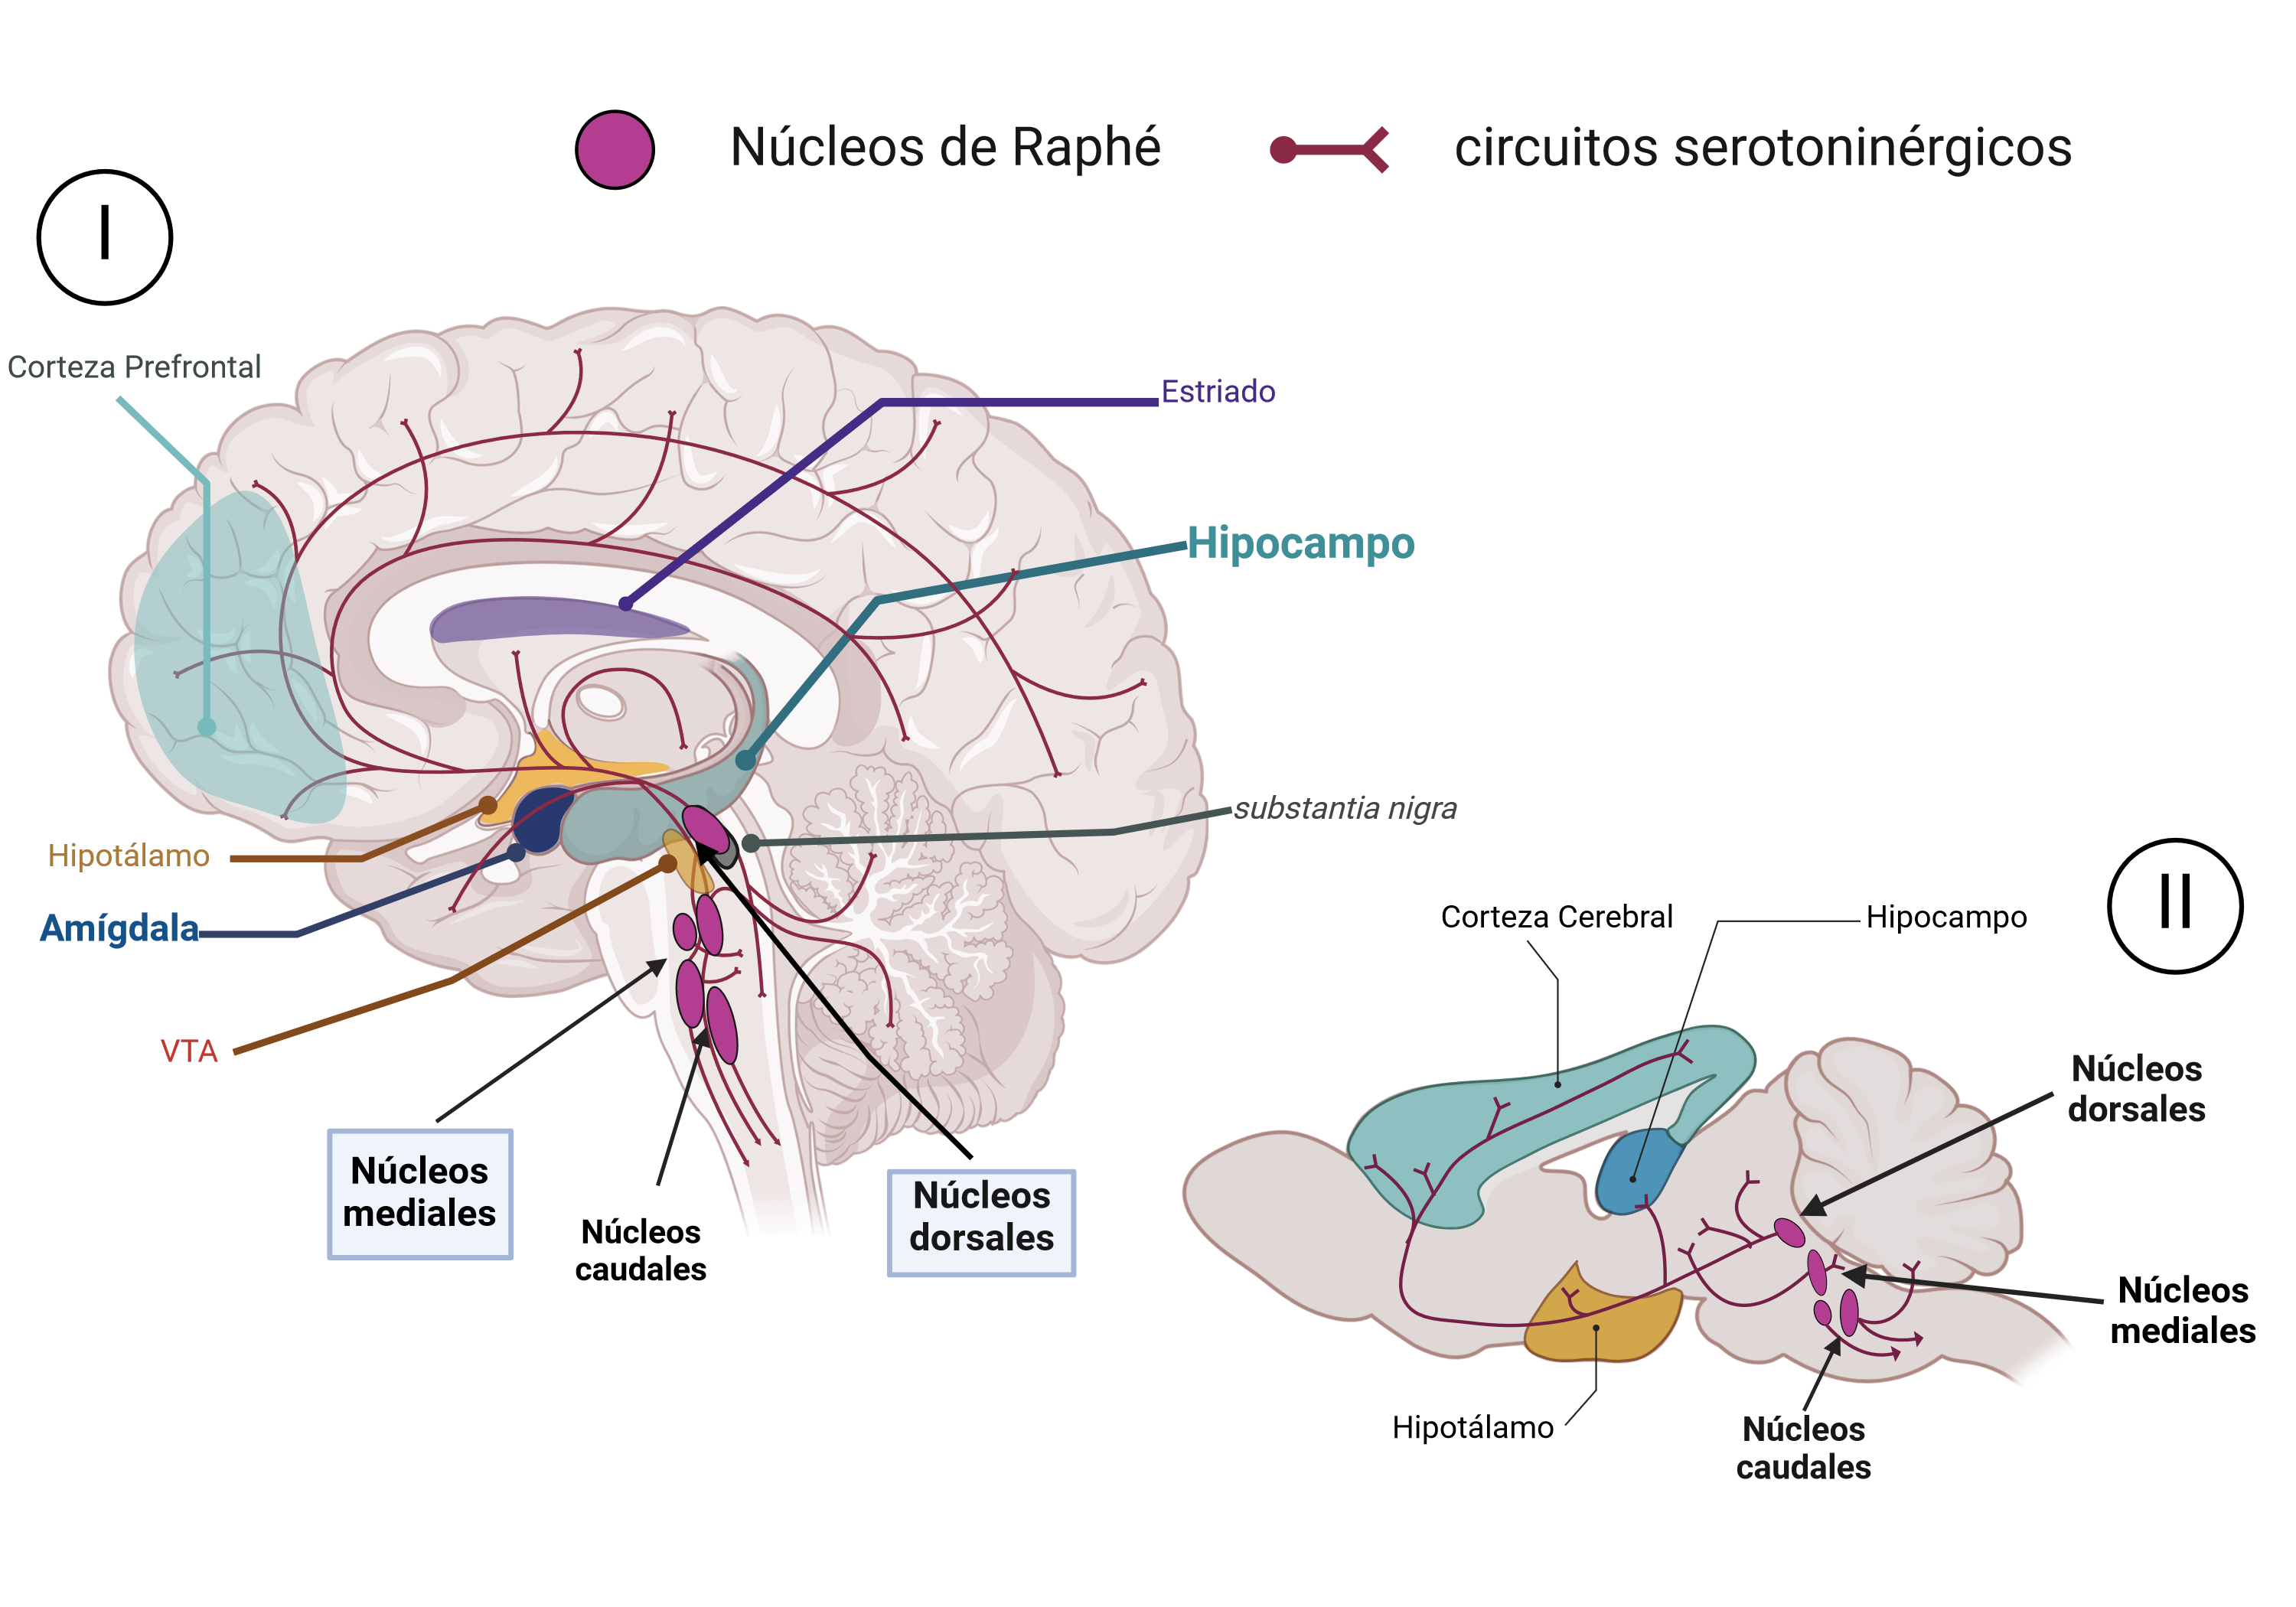
\includegraphics[width=0.8\linewidth,height=\textheight,keepaspectratio]{../Figures/raphe.png}

}

\caption[Proyecciones serotoninérgicas de los núcleos de
Rafé]{\label{fig-raphe}Proyecciones serotoninérgicas de los núcleos de
Rafé hacia áreas cerebrales involucradas en la regulación de la memoria
y las emociones. La figura presenta una vista esquemática de los núcleos
de Rafé y sus proyecciones serotoninérgicas en corte sagital de I)
cerebro humano y II) cerebro de roedor. Se observa que los núcleos de
Rafé están ubicados en el tronco encefálico. Desde estos núcleos, las
fibras serotoninérgicas proyectan hacia diversas regiones:
\textbf{Corteza Prefrontal}: Involucrada en funciones ejecutivas (p.~ej.
atención, recuperación de memorias) y regulación emocional.
\textbf{Hipotálamo}: Importante en la regulación del estrés y las
respuestas autónomas. \textbf{Amígdala}: Crítica para la formación de
recuerdos emocionales (p.~ej. miedo). \textbf{Hipocampo}: Fundamental
para la formación y recuperación de memorias episódicas.
\textbf{Estriado}: Implicado en la modulación de las funciones motoras y
de recompensa. \textbf{Área Tegmental Ventral}: Relacionada con la
recompensa y la motivación. Información tomada de: @hornung2003;
@waselus2011; @alenina2015; @levinson2023}

\end{figure}%

La biosíntesis de \ac{5-ht} implica la hidroxilación y descarboxilación
del triptófano, un aminoácido esencial {[}@hale2011{]}. En un primer
paso, el triptófano es convertido en \ac{5-htp} mediante la enzima
\ac{tph}, la cual determina la tasa de producción de \ac{5-ht} debido a
su cinética constitutivamente lenta. En un segundo paso, el \ac{5-htp}
se convierte a \ac{5-ht} a través de la acción de la enzima \ac{aaad}
{[}@roth2021{]}. Esta regulación biosintética de la \ac{5-ht} puede
verse profundamente afectada por factores externos, como el estrés. Los
niveles elevados de cortisol, como los observados durante el estrés
crónico, provocan una disminución en los niveles de \ac{5-ht} en el
sistema nervioso {[}@chen2017b{]}. Este efecto se debe a un mecanismo
que involucra la \colorbox{BurntOrange}{inhibición de la enzima}
\ac{tph}-2 (Figure~\ref{fig-tph2}) {[}@shimomura2019{]}, la isoforma de
\ac{tph} que se encuentra en las neuronas serotoninérgicas
{[}@lowry2008{]}.

\begin{figure}

\begin{minipage}{0.47\linewidth}

\begin{figure}[H]

\centering{

\pandocbounded{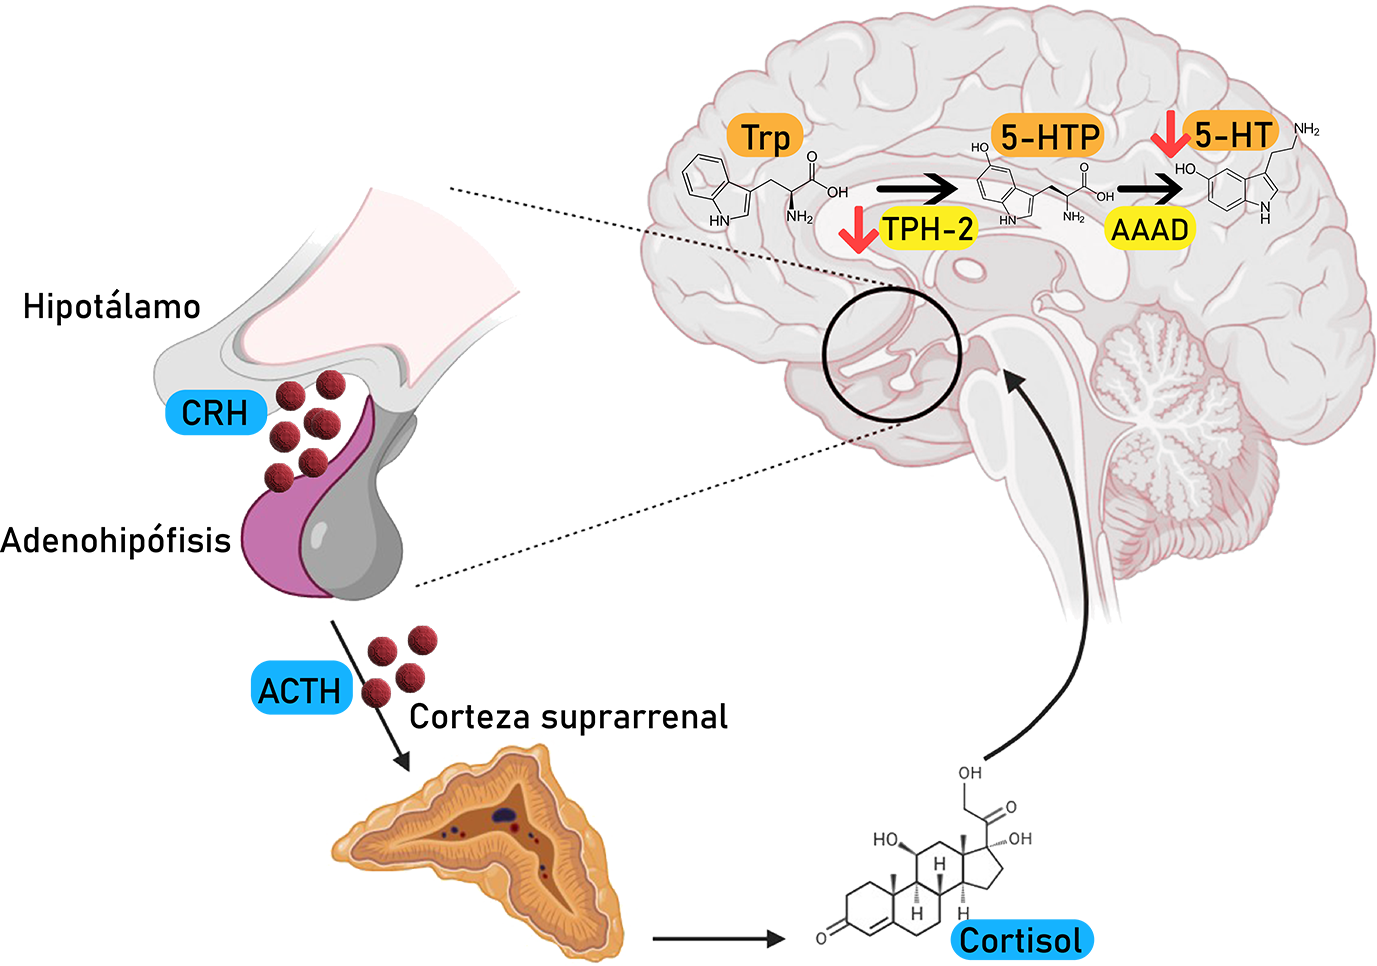
\includegraphics[keepaspectratio]{../Figures/tph2_estres.png}}

}

\caption{\label{fig-tph2}Respuesta al Estrés y efectos del Cortisol
sobre el sistema serotoninérgico del sistema nervioso.}

\end{figure}%

\end{minipage}%
%
\begin{minipage}{0.05\linewidth}
~\end{minipage}%
%
\begin{minipage}{0.47\linewidth}
La figura ilustra cómo el estrés crónico activa la liberación de la
\ac{crh} y \ac{acth}, elevando los niveles de cortisol. {[}@hale2011;
@chen2013{]}. El aumento sostenido de cortisol en el cuerpo tiene un
efecto inhibidor sobre la actividad de la \ac{tph}-2, reduciendo los
niveles de \ac{5-ht} en el cerebro {[}@shimomura2019{]}. La disminución
de los niveles de \ac{5-ht} está vinculada a la aparición de trastornos
depresivos {[}@chen2017b{]}. Información tomada de @hale2011 y
@chen2013\end{minipage}%

\end{figure}%

Existe evidencia de que los fármacos antidepresivos
\colorbox{BurntOrange}{clásicos, conocidos como} \ac{isrs} modulan la
actividad de la \ac{tph}-2 y aumentan la disponibilidad de \ac{5-ht} en
el cerebro {[}@chen2017b{]}. Además, se ha visto que la actividad de la
\ac{tph}-2 regula la \ac{nha} y los comportamientos de tipo ansioso en
un modelo murino {[}@kanai2009{]}. Sin embargo, el mecanismo exacto
entre la \ac{tph}-2, la \ac{nha} y los \ac{isrs} no se ha comprendido
completamente {[}@song2016{]}. Por un lado, los \ac{isrs} actúan a
través del sistema serotoninérgico y promueven la \ac{nha}
{[}@malberg2000{]}. Por otro lado, la disminución de \ac{5-ht} está
asociada con una reducción en el número de células recién generadas en
el \ac{gd} {[}@brezun1999{]}. Los receptores serotoninérgicos 5-HT1A,
5-HT2B y 5-HT2C (Figure~\ref{fig-neurogenesis}) son candidatos
destacados para contribuir a la respuesta antidepresiva ya que regulan
el desarrollo normal de la densidad de espinas dendríticas y la
formación de sinapsis en las células granulares en el \ac{gd}, y median
la maduración de las células progenitoras {[}@alenina2015{]}.

\begin{figure}

\centering{

\pandocbounded{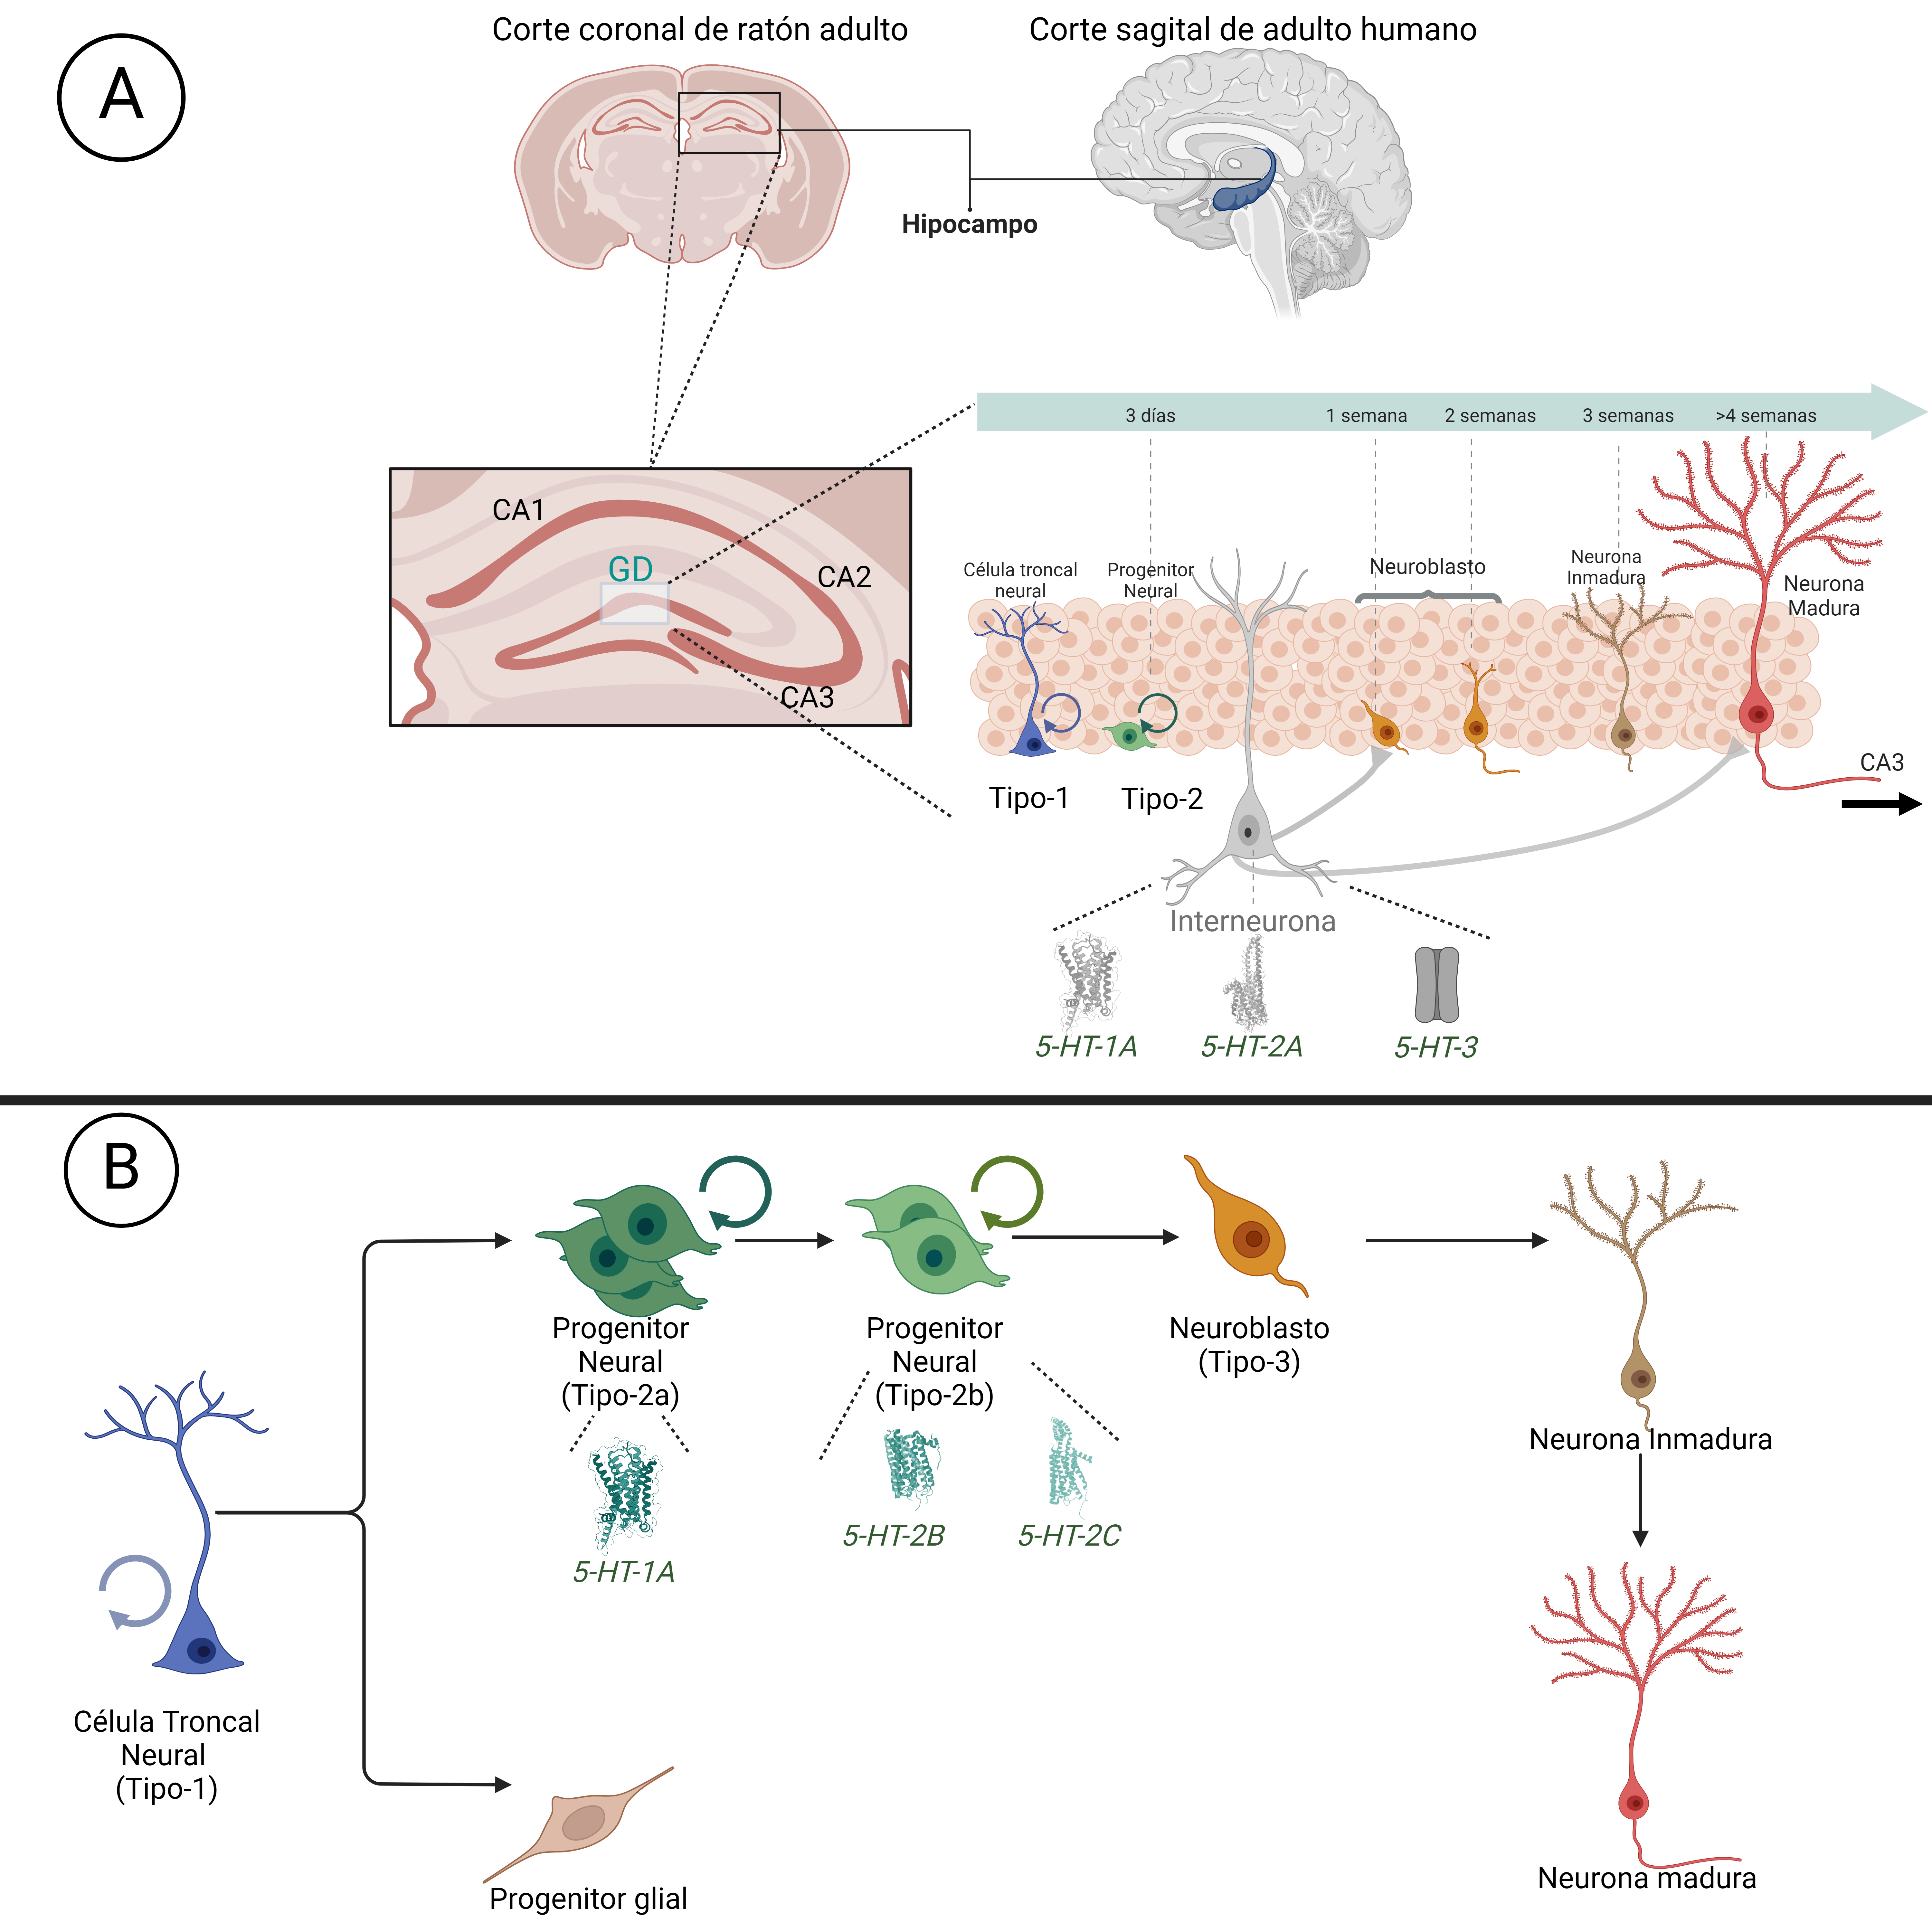
\includegraphics[keepaspectratio]{../Figures/neurogenesis.png}}

}

\caption[Neurogénesis adulta y expresión de receptores de
\ac{5-ht}]{\label{fig-neurogenesis}Ciclo de neurogénesis adulta en el
\ac{gd} y expresión de receptores de \ac{5-ht}. A) Diagrama del
hipocampo mostrando el \ac{gd} y la dinámica de la neurogénesis adulta
{[}@denoth-lippuner2021{]}: se muestra la ubicación del \ac{gd} y se
ilustra el proceso de la \ac{nha}, desde las células madre neurales
hasta la integración de neuronas maduras en el circuito neural.
\emph{Células troncales neurales}: Localizadas en la capa subgranular,
estas células proliferan y se diferencian en progenitores neuronales.
\emph{Neuroblastos}: En las siguientes semanas, los neuroblastos migran
y se desarrollan en neuronas inmaduras. \emph{Neuronas maduras}: Después
de más de cuatro semanas, las neuronas maduras se integran en la región
\ac{ca}3 del hipocampo, formando conexiones sinápticas funcionales. B)
Expresión de diferentes receptores de \ac{5-ht} en las células del
\ac{gd} durante su desarrollo y maduración {[}@song2016; @batool2019{]}:
el receptor \emph{5-HT1A} se expresa en las etapas tempranas de las
células progenitoras; los receptores \emph{5-HT2B} y \emph{5-HT2C} se
expresan en las células progenitoras; el receptor ionotrópico
\emph{5-HT3} se encuentra principalmente en las interneuronas del
\ac{gd}. Información tomada de @alenina2015 y @song2016}

\end{figure}%

La interacción del sistema serotoninérgico con la \ac{nha} también se
refleja en estudios \emph{post mortem} {[}@boldrini2009; @boldrini2012;
@boldrini2013{]}, proporcionando un mayor entendimiento sobre el impacto
de los antidepresivos en el cerebro. Estos estudios indican que los
pacientes depresivos medicados con antidepresivos tienen más marcadores
de NHA en comparación con pacientes no medicados. Finalmente, la
flexibilidad cognitiva se beneficia de la plasticidad inducida por esta
neurogénesis modulada por la \ac{5-ht} {[}@burghardt2012; @anacker2017;
@hurtubise2017; @matias2017; @marwari2018; @doss2021{]}. Bajo
condiciones ambientales adecuadas (no aversivas) {[}@branchi2011;
@genet2013; @carhart-harris2018; @magaraggia2021; @branchi2022;
@jacobsen2023{]}, esta plasticidad neuronal puede promover nuevas
asociaciones y mejorar las distorsiones cognitivas (p.~ej.
\href{AppendixB.qmd\#term-id-70}{rumiaciones}) {[}@mahar2014{]} que
perpetúan y agravan los trastornos de ansiedad y depresión
{[}@guler2022{]}.

\begin{tcolorbox}[enhanced jigsaw, colframe=quarto-callout-warning-color-frame, left=2mm, bottomrule=.15mm, rightrule=.15mm, arc=.35mm, toprule=.15mm, leftrule=.75mm, breakable, opacityback=0, colback=white]

\vspace{-3mm}\textbf{\textbf{Fármacos Antidepresivos}}\vspace{3mm}

Los primeros antidepresivos desarrollados fueron los inhibidores de la
monoamino oxidasa, que mejoraban el ánimo a costa de efectos secundarios
importantes, como toxicidad hepática y crisis hipertensivas
{[}@lopez-munoz2009{]}. Posteriormente, se desarrollaron los
antidepresivos tricíclicos como la imipramina, que actúan principalmente
bloqueando la recaptura de \ac{5-ht} y noradrenalina. Debido a su falta
de especificidad y efectos secundarios, los antidepresivos tricíclicos
se prescriben actualmente para casos muy particulares de depresión
{[}@hillhouse2015{]}. A finales de los años 80, surgieron los
antidepresivos de segunda generación, incluyendo los \ac{isrs} y los
inhibidores de la recaptación de \ac{5-ht} y noradrenalina
{[}@hanson2011{]}. Los \ac{isrs}, como el escitalopram, la fluoxetina y
la sertralina, son los medicamentos más recetados para los trastornos de
depresión y ansiedad {[}@latest\_lin\_2023{]}.

Su mecanismo de acción inmediato es a través de la regularización del
sistema serotoninérgico mediante el incremento de la concentración de
\ac{5-ht} en el espacio sináptico, a través de la inhibición de la
recaptura de este neurotransmisor por el \ac{sert}
(Figure~\ref{fig-ssri}). Sin embargo, se ha sugerido que su mecanismo de
acción antidepresiva involucra el aumento en la \ac{nha}
{[}@santarelli2003; @tunc-ozcan2019{]} que a su vez se ha relacionado
con promover la flexibilidad cognitiva (Figure~\ref{fig-flexneuro};
Figure~\ref{fig-neurogenesis}) {[}@burghardt2012; @marwari2018;
@maramis2021{]}. Como se mencionó antes (Section~\ref{sec-nha}), esta
flexibilidad mejora la capacidad para adaptarse a nuevas situaciones y
experiencias, resultando en una reducción de síntomas depresivos y
ansiosos y una mejora en el ánimo (Figure~\ref{fig-flexibilidad}).

\begin{figure}[H]

\centering{

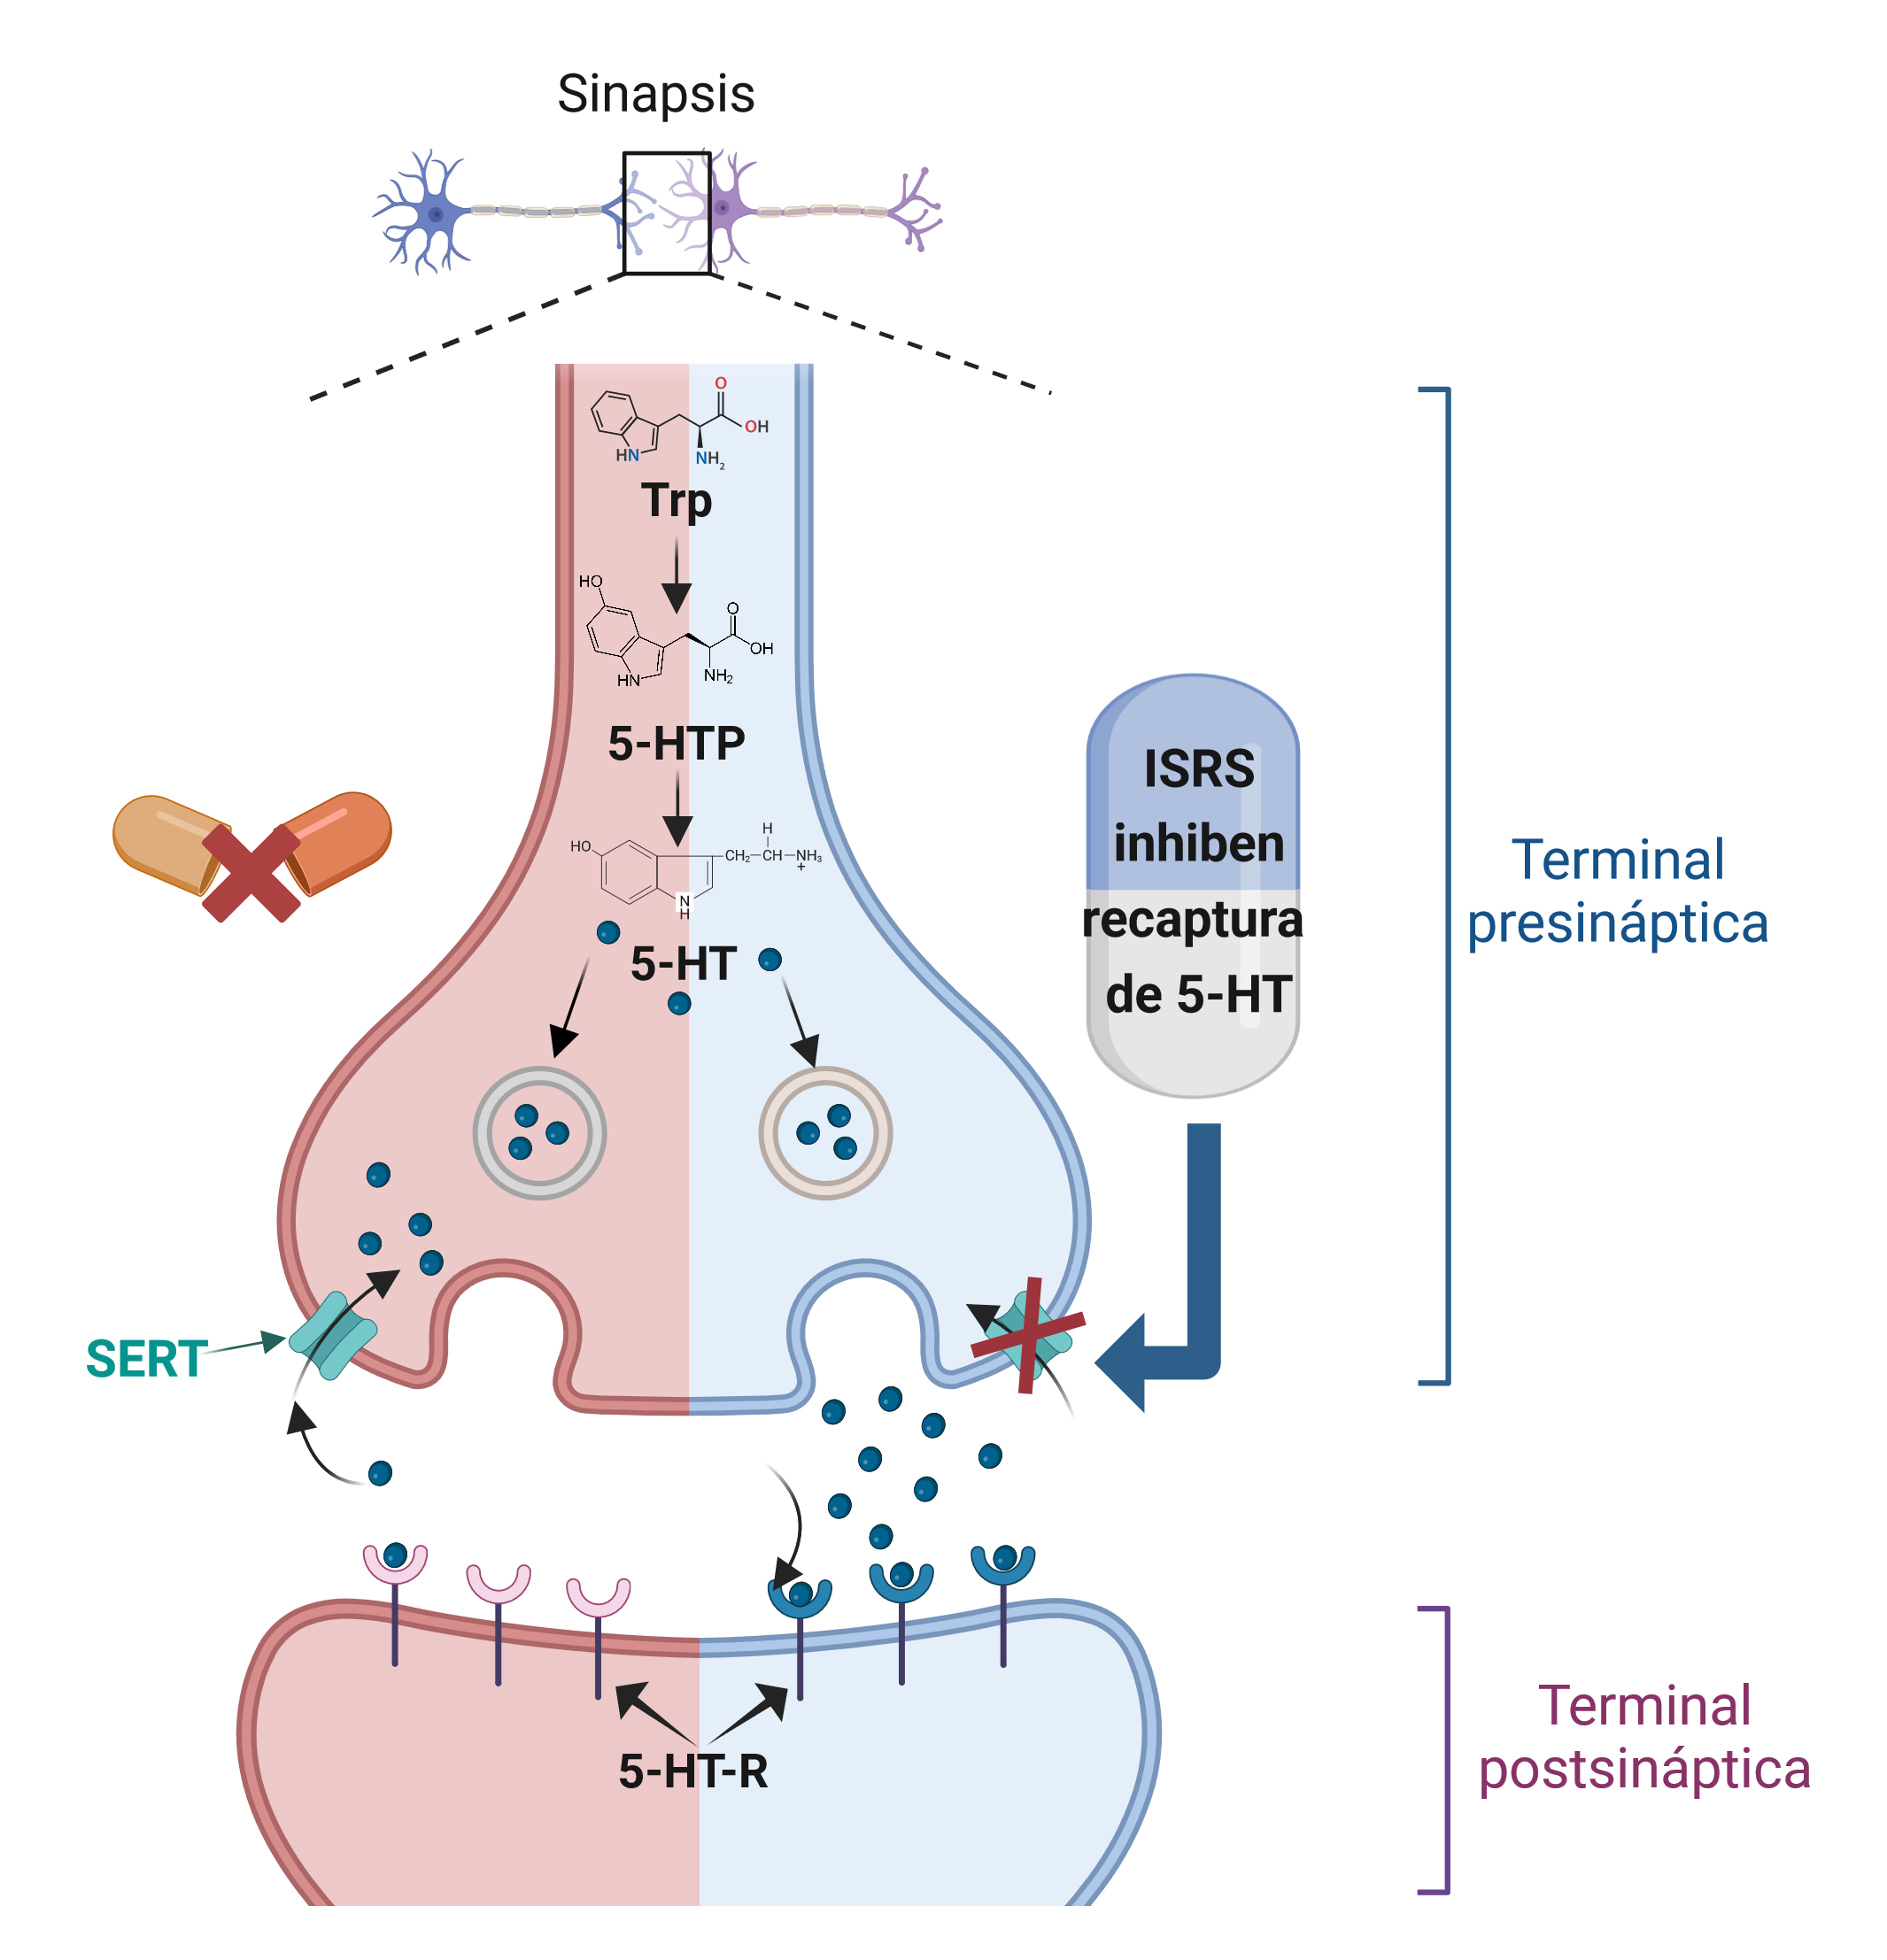
\includegraphics[width=0.9\linewidth,height=\textheight,keepaspectratio]{../Figures/ssri.png}

}

\caption[Mecanismo de acción de los fármacos antidepresivos
clásicos]{\label{fig-ssri}Mecanismo de acción de los \ac{isrs} en la
sinapsis. Se ilustra el mecanismo de acción de los \ac{isrs}, comparando
una sinapsis sin la presencia de estos medicamentos (lado izquierdo,
fondo rojo) con una sinapsis en presencia de \ac{isrs} (lado derecho,
fondo azul). En la terminal presináptica, el triptófano (Trp) es
convertido en \ac{5-htp} por la acción de la \ac{tph}. El \ac{5-htp} se
convierte en \ac{5-ht} por la acción de la \ac{aaad}. \emph{Sinapsis sin
\ac{isrs} (lado izquierdo)}: La \ac{5-ht} es almacenada en vesículas y
liberada en la hendidura sináptica en respuesta a un potencial de
acción. Parte de la \ac{5-ht} liberada se une a los receptores de
\ac{5-ht} en la membrana postsináptica, facilitando la transmisión de la
señal. La \ac{5-ht} sobrante es recapturada en la terminal presináptica
por el \ac{sert}, reduciendo su disponibilidad en la sinapsis.
\emph{Sinapsis con \ac{isrs} (lado derecho)}: Los \ac{isrs} bloquean el
\ac{sert} en la terminal presináptica, impidiendo la recaptura de
\ac{5-ht}. Esto aumenta la disponibilidad de \ac{5-ht} en la hendidura
sináptica. La mayor concentración de \ac{5-ht} permite una mayor
interacción con los receptores de \ac{5-ht} postsinápticos (5-HT-R),
potenciando la transmisión de señales neuronales. Este mecanismo es
fundamental para la eficacia terapéutica de los \ac{isrs} en el
tratamiento de trastornos depresivos y de ansiedad, como se describe en
los estudios de @mahar2014 y @alenina2015. Figura basada en @loke2021}

\end{figure}%

\end{tcolorbox}




\end{document}
